\documentclass{article}
\usepackage[english]{babel}
\usepackage[a4paper,top=2cm,bottom=2cm,left=3cm,right=3cm,marginparwidth=1.75cm]{geometry}

% Useful packages
\usepackage{amsmath}
\usepackage{graphicx}
\usepackage{float}
\usepackage[colorlinks=true, allcolors=blue]{hyperref}

\title{Book F1 - 2024}
\author{AIMI Laora}
\date{}

\begin{document}
\maketitle


\section*{Introduction}

This document is a thorough report on the 2024 Formula 1 World Championship from a race-by-race perspective. Each Grand Prix consists of two main sections:

\begin{itemize}
    \item \textbf{Circuit Analysis} — The circuit layout is presented, along with its specific character, strategic challenges (specific braking zones, tyre degradation, overtaking zones, DRS zones, and some weather context).
    \item \textbf{Race Analysis} — The section provides a summary of qualifying and race results, the major incidents, the strategies the teams used, the trends in performance, and the implications of the championship. Each analysis ends with a Takeaway, identifying the key factors from the results of the event, primarily for lessons learned.
\end{itemize}

The objective is not only to record the results of the 2024 season, but also to identify broader
performance trends, strategic choices, and turning points that shaped the battle between drivers
and constructors.

The end of season review includes a global synthesis outlines:
\begin{itemize}
    \item The main competitive trends of the year,
    \item The biggest surprises and disappointments,
    \item A team-by-team evaluation of performance.
\end{itemize}

This contributes to summarising the full season, comparing an overview of both the technical and strategic distance traveled by the racers and constructors together over the course of a season.



\section{Bahrain Grand prix}

\subsection{Circuit Analysis}

\textbf{Circuit Name:} Bahrain International Circuit (Sakhir, Bahrain) \\
\textbf{Length:} 5.412 km - \textbf{Laps:} 57 - \textbf{Total Distance:} 308.238 km

\begin{figure}[H]
    \centering
    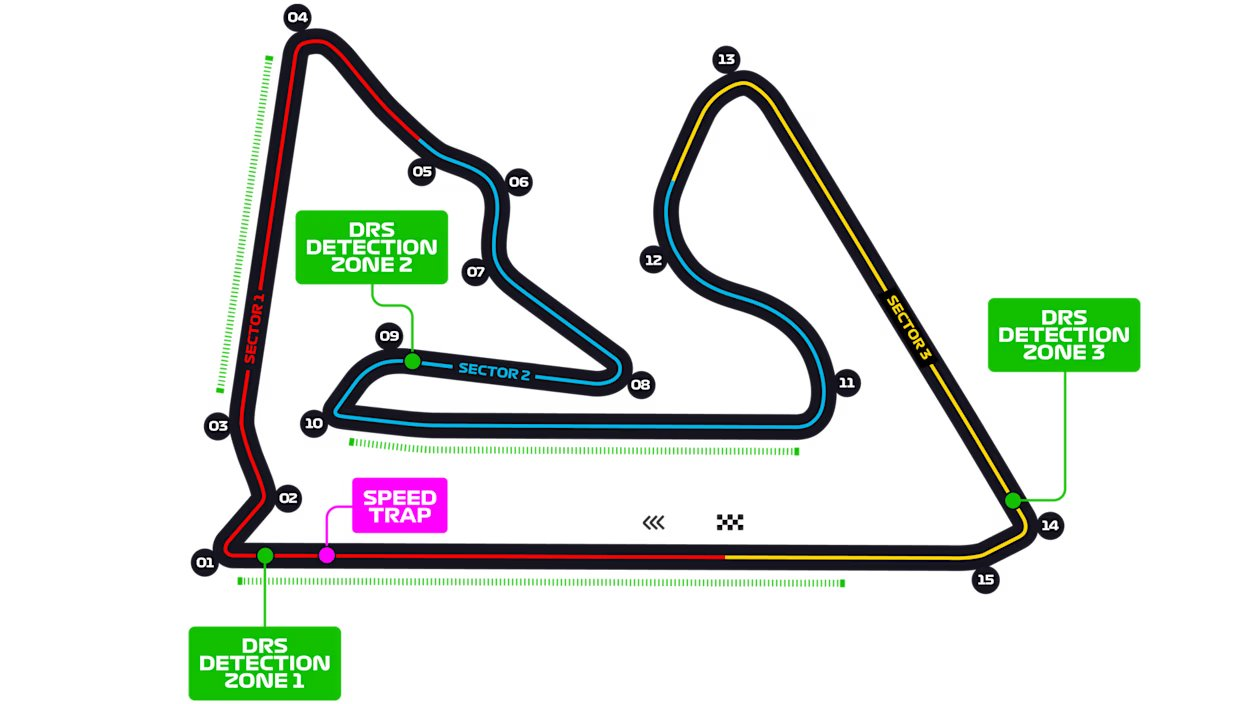
\includegraphics[width=0.75\linewidth]{images/1.Bahrain_Circuit.jpg}
\end{figure}

\begin{itemize}
    \item \textbf{Lap Record} : 1:27.264 (2020, Lewis Hamilton - Mercedes).
    
    \item \textbf{Number of Corners \& Key Features} : 15 turns (9 right, 6 left) - Track offers long straights, heavy braking zones (Turns 1, 4 \& 14), and technical sections like Turn 10 (off-camber, downhill)—key for grip and balance.
    
    \item \textbf{Braking Zones \& Traction} : Drivers brake from over 300 km/h to ~60 km/h in crucial zones, requiring extreme precision.\\
    Turn 10 particularly punishes front-left tyre instability.
    
    \item \textbf{DRS \& Overtaking} : Three DRS zones: along main straight, near Turn 4, and around Turn 10 areas. \\
    Combined with heavy braking zones, the track enables solid overtaking opportunities.
    
    \item \textbf{Tyre Degradation \& Strategy} : Teams chose mostly hard and soft compounds, medium rarely used. \\
    Two-stop strategies dominated: Soft–Hard–Soft or Soft–Hard–Hard favoured.
    
    \item \textbf{Weather \& Environment} : Night race with significant temperature swings and desert wind affects grip, braking stability, and tyre management.
\end{itemize}

\textbf{Strategic Summary :}
Bahrain demands cars with strong braking stability, rear traction, and efficient thermal regime. Tyre management and race pace outperform starting position, making flexible two-stop strategies (starting on softs, moving to hard) highly effective. The technical Turn 10 differentiates driver and car setups, while environmental factors add strategic layers.


\subsection{Race Analysis}

\textbf{Date:} 2 March 2024 — 18:00 local time 

\begin{itemize}
    \item \textbf{Qualifying Summary} : \textbf{Pole Position:} Max Verstappen (Red Bull) – 1:29.179. \\
    Grid: Leclerc 2nd, Russell 3rd, Sainz 4th.\\
    Top nine within half a second (tight field).
    
    \item \textbf{Race Summary} : \textbf{Winner:} Max Verstappen (Red Bull) - dominant, led every lap, and secured fastest lap\\
    \textbf{Podium:} 1. Verstappen - 2. Pérez - 3. Sainz.\\
    No retirements - rare in a season opener.\\
    \textbf{Technical issues:} Leclerc (brakes), Mercedes (ERS).
    
    \item \textbf{Strategies} : Two-stop norm (Soft–Hard–Hard / Soft–Hard–Soft). \\
    - Red Bull extended stints to pit later than rivals, keeping Verstappen in clear air. \\
    - Ferrari limited by Leclerc’s brake instability, Sainz maximised tyre life and overtaking ability. \\
    - McLaren lacked raw pace but executed consistent strategies.
    
    \item \textbf{Performance Trends} : \textbf{Red Bull} — absolute dominance, RB20 strong in braking and tyre management. \\
    \textbf{Ferrari} — Sainz competitive (P3, “Driver of the Day”), Leclerc compromised by braking issues at Turn 10. \\
    \textbf{Mercedes} — good quali (Russell P3) but race pace dropped with overheating. Hamilton limited to P7. \\
    \textbf{McLaren} — Norris (P6) and Piastri (P8) consistent but off the podium fight. \\
    \textbf{Aston Martin} — Alonso P9, Stroll P10, not enough pace for higher points. 
    
    \item \textbf{Championship Impact} : \textbf{Drivers:} Verstappen opened with 26 points; Pérez and Sainz close behind.\\
    \textbf{Constructors:} Red Bull 44, Ferrari 27, Mercedes 16, McLaren 12.    
\end{itemize}

\textbf{Key Takeaway :}
Red Bull’s superior car performance, efficient soft-tyre use, and masterful race pace translated directly into season-opening dominance. Meanwhile, the circuit’s demands exposed weaknesses in other teams, especially regarding brake management and strategy flexibility.


\subsection{Link \& Takeaway}

\begin{itemize}
    \item Turn 10’s brake demands directly shaped Leclerc’s race, showing the circuit’s technical brutality. 
    \item Red Bull maximised Bahrain’s tyre-heavy layout with late pit stops and soft-tyre exploitation. 
    \item Ferrari’s contrasting fortunes (Sainz consistency vs. Leclerc brake issues) revealed limits of the SF-24. 
    \item Historic opener: no DNFs — emphasising reliability improvements across the grid.
\end{itemize}

\section{Saudi Arabian Grand prix}

\subsection{Circuit Analysis}

\textbf{Circuit Name:} Jeddah Corniche Circuit (Jeddah, Saudi Arabia) \\
\textbf{Length:} 6.174 km - \textbf{Laps:} 50 - \textbf{Total Distance:} 308.450 km

\begin{figure}[H]
    \centering
    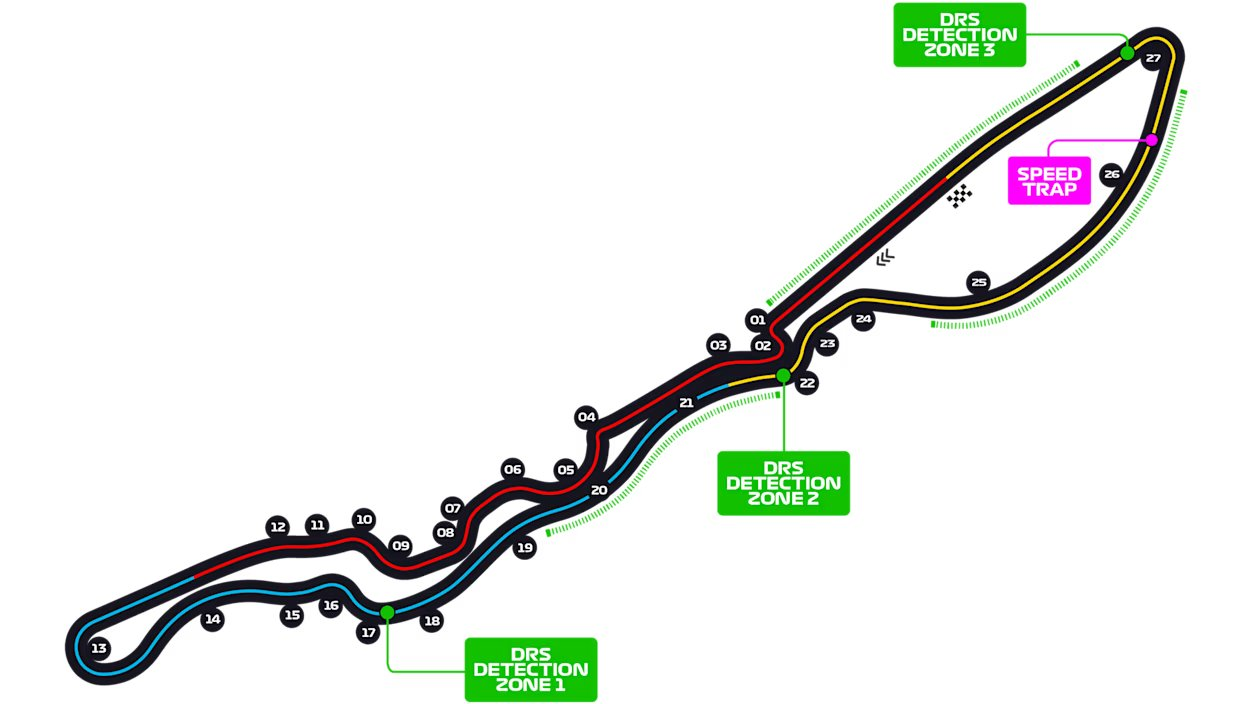
\includegraphics[width=0.75\linewidth]{images/2.Jeddah_Circuit.jpg}
\end{figure}

\begin{itemize}
    \item \textbf{Lap Record} : 1:27.511 (2021, Lewis Hamilton - Mercedes).
    
    \item \textbf{Number of Corners \& Key Features} : 27 turns (11 right, 16 left)  - High-speed kinks, extremely tight margins, walls very close to the track.\\
    Predominantly high-speed corners, including challenging sections like Turn 10 and Turn 22 with limited visibility.\\
    \textbf{Fastest corner (Turn 13)} can be taken at 322 km/h, with a 12° slope.
    
    \item \textbf{Braking Zones \& Traction} : Only 7 braking points per lap: 2 heavy, 2 medium, 3 light.\\
    \textbf{Most demanding zones:} Turns 1 (317→110 km/h), 22, and 27.
    
    \item \textbf{DRS \& Overtaking} : Three DRS zones: along main straight, near Turn 21, and before the final corner. \\
    Despite the DRS, only Turns 1 and 27 account for 89\% of overtakes in data.
    
    \item \textbf{Tyre Degradation \& Strategy} : Low tyre degradation allows one-stop strategies, especially with medium/hard compounds. \\
    High likelihood of Safety Car due to narrow corridors and close barriers.
    
    \item \textbf{Weather \& Environment} : Night race under powerful lighting; temperatures drop significantly at night, affecting tyre grip and brake cooling.\\
    Proximity to desert means wind and sand can affect grip unpredictably.
\end{itemize}

\textbf{Strategic Summary :}
The Jeddah track demands cars with engine power, straight-line speed, stability at high velocity, and precision through kink-heavy sectors. Overtaking is concentrated around heavily-braked zones, and teams must be ready for Safety Car-induced strategic shifts. One-stop strategies are usually viable, but environmental effects like sand dust and temperature swings cannot be ignored.


\subsection{Race Analysis}

\textbf{Date:} 9 March 2024 — 20:00 local time 

\begin{itemize}
    \item \textbf{Qualifying Summary} : \textbf{Pole Position:} Max Verstappen (Red Bull) – 1:27.472 (new track record). \\
    Grid: Leclerc 2nd, Pérez 3rd, Alonso 4th.\\
    Notable: Rookie Oliver Bearman (Ferrari, replacing Sainz – appendicitis) qualified P11.
    
    \item \textbf{Race Summary} : \textbf{Winner:} Max Verstappen (Red Bull). \\
    \textbf{Podium:} 1. Verstappen - 2. Pérez - 3. Leclerc.\\
    \textbf{Technical issues:} Gasly (gearbox - retired formation lap).\\
    \textbf{Notable incidents:} Stroll crashed at Turn 14 (Safety Car lap 7).\\
    Rookie Bearman finished P7 on debut, scoring 6 points for Ferrari.
    
    \item \textbf{Strategies} : 
    - Teams mostly opted for one-stop strategies, using medium tyres for the first stint.\\
    - Medium durability allowed extended stints. 
    - Some switched to softs late for speed.
    
    \item \textbf{Performance Trends} : \textbf{Red Bull} — Dominant again, securing a second 1–2 despite Pérez’s 5s penalty. Verstappen unchallenged (45 laps led). \\
    \textbf{Ferrari} — Leclerc maximised P3 + fastest lap. Rookie Bearman impressed with calm, consistent debut drive to P7. \\
    \textbf{McLaren} — Piastri P4, Norris P8, competitive but not podium-level. \\
    \textbf{Mercedes} — Russell P6, Hamilton P9, solid points but lack of pace in straights evident. \\
    \textbf{Aston Martin} — Alonso P5, Stroll retired after crash. \\
    \textbf{Haas} — Hülkenberg P10, first point of the year. 
    
    \item \textbf{Championship Impact} : \textbf{Drivers:} Verstappen 51 points, Pérez 36, Leclerc 28 (+1).\\
    \textbf{Constructors:} Red Bull 87, Ferrari 49, McLaren 28 (+1), Mercedes 26 (-1).    
\end{itemize}

\textbf{Key Takeaway :}
Verstappen extended his winning streak with complete control. Pérez salvaged P2 despite a penalty, while Leclerc and Ferrari optimised points. Bearman’s surprise debut and points finish provided the human highlight of the weekend.


\subsection{Link \& Takeaway}

\begin{itemize}
    \item High-speed layout perfectly matched Red Bull’s strengths in aero efficiency and straight-line speed. 
    \item One-stop strategy confirmed Jeddah’s low tyre wear, with little variation in pit calls. 
    \item Safety Car briefly reshuffled order but didn’t threaten Verstappen’s dominance. 
    \item Bearman’s debut became the story of the weekend, contrasting with Red Bull’s overwhelming control. 
    \item Overtaking limited to key braking zones, the safety car period (after Stroll's crash) didn’t significantly disrupt the top order.
\end{itemize}
\section{Australian Grand prix}

\subsection{Circuit Analysis}

\textbf{Circuit Name:} Albert Park Grand Prix Circuit (Melbourne, Australia) \\
\textbf{Length:} 5.278 km - \textbf{Laps:} 58 - \textbf{Total Distance:} 306.124 km

\begin{figure}[H]
    \centering
    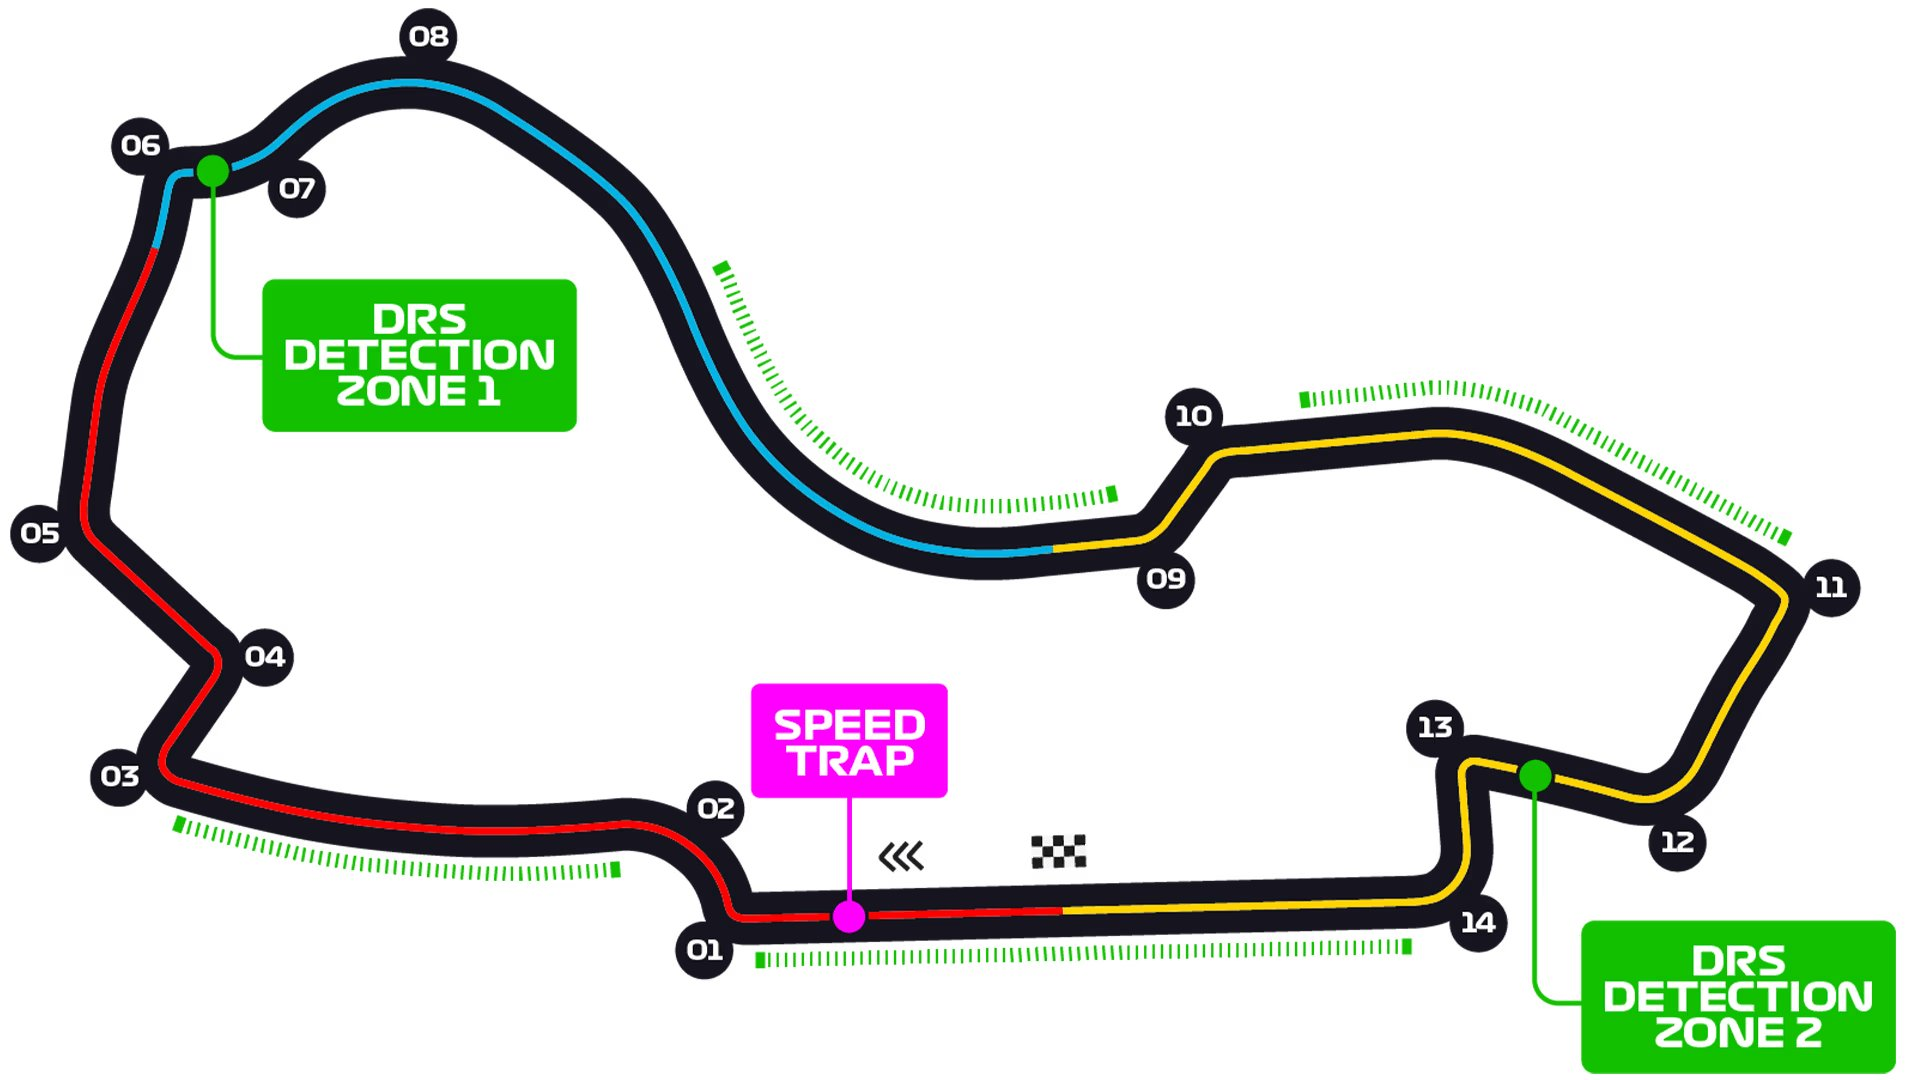
\includegraphics[width=0.75\linewidth]{images/3.Australia_Circuit.jpg}
\end{figure}

\begin{itemize}
    \item \textbf{Lap Record} : 1:16.732 (2023, Max Verstappen - Red Bull).
    
    \item \textbf{Number of Corners \& Key Features} : 16 turns (10 right, 6 left) - Tight, flowing corners.\\
    Barriers close to the track make errors costly.
    
    \item \textbf{Braking Zones \& Traction} : Several intense braking zones (e.g., Turn 1 into Turn 2 is a challenging sequence)
    
    \item \textbf{DRS \& Overtaking} : Four DRS zones: along main straight, between Turns 2 and 3, before Turn 8 and between Turns 10 and 11. \\
    Not heavy on overtaking despite having some DRS zones, primarily at Turns 1, 3, 13.
    
    \item \textbf{Tyre Degradation \& Strategy} : Tyre degradation is low, but tyre management (especially avoiding graining) is crucial.

    \item \textbf{Weather \& Environment} : Most of the time, this is a sunny weekend. Track often dusty at start of weekend.
\end{itemize}

\textbf{Strategic Summary :}
Albert Park rewards consistency, tyre preservation, and precision. Its smooth surface and moderate degradation allow varied strategies. Cars with well-balanced downforce (to handle mid-speed corners and braking) tend to do well.


\subsection{Race Analysis}

\textbf{Date:} 24 March 2024 — 15:00 local time 

\begin{itemize}
    \item \textbf{Qualifying Summary} : \textbf{Pole Position:} Max Verstappen (Red Bull) – 1:15.915 (new track record). \\
    Grid: Sainz 2nd, Norris 3rd, Leclerc 4th.\\
    Sergio Pérez, who finished 3rd during the qualifications, was penalised of three grid places for impeding.
    
    \item \textbf{Race Summary} : \textbf{Winner:} Carlos Sainz (Ferrari). \\
    \textbf{Podium:} 1. Sainz - 2. Leclerc - 3. Norris.\\
    \textbf{Technical issues:} Verstappen (brake-related mechanical failure - retired lap 3), Hamilton (engine).\\
    \textbf{Notable incidents:} Russell crashed because of Alonso (20s penalty) (Virtual Safety Car last lap).
    
    \item \textbf{Strategies} : Most runners began on medium tyres, switching to hards.\\
    - Ferrari managed tyre graining well. Sainz extended his first stint early to build a gap.\\
    - Leclerc executed a successful undercut on Norris.
    
    \item \textbf{Performance Trends} :\textbf{Ferrari} — Flawless execution: first 1–2 finish since Bahrain 2022. Sainz voted Driver of the Day. \\
    \textbf{McLaren} — Strong pace, Norris podium, Piastri close behind. \\
    \textbf{Red Bull} — Pérez distant P5, Verstappen retired early. \\
    \textbf{Mercedes} — Double DNF: Hamilton engine failure, Russell crash. First since Austria 2018.\\
    \textbf{Haas} — Double points: Hülkenberg P9, Magnussen P10. 
    
    \item \textbf{Championship Impact} : \textbf{Drivers:} Verstappen 51 points, Leclerc 47 (+1), Pérez 46 (-1).\\
    \textbf{Constructors:} Red Bull 97, Ferrari 93, McLaren 55, Mercedes 26.
\end{itemize}

\textbf{Key Takeaway :}
Ferrari capitalised on Red Bull’s misfortune and delivered a flawless strategic execution. Sainz in particular controlled tyre wear superbly, while Leclerc’s undercut secured the team valuable points.


\subsection{Link \& Takeaway}

\begin{itemize}
    \item The circuit’s low degradation meant strategic advantage went to those who conserved tyres, Ferrari mastered this, extending stints and minimising graining.
    \item The semi-street layout requires well-balanced cars for corners, Ferrari’s setup gave them the edge. McLaren and Red Bull lagged in consistent performance.
\end{itemize}
\section{Japanese Grand prix}

\subsection{Circuit Analysis}

\textbf{Circuit Name:} Suzuka International Racing Course (Suzuka, Japan) \\
\textbf{Length:} 5.807 km - \textbf{Laps:} 53 - \textbf{Total Distance:} 307.471 km

\begin{figure}[H]
    \centering
    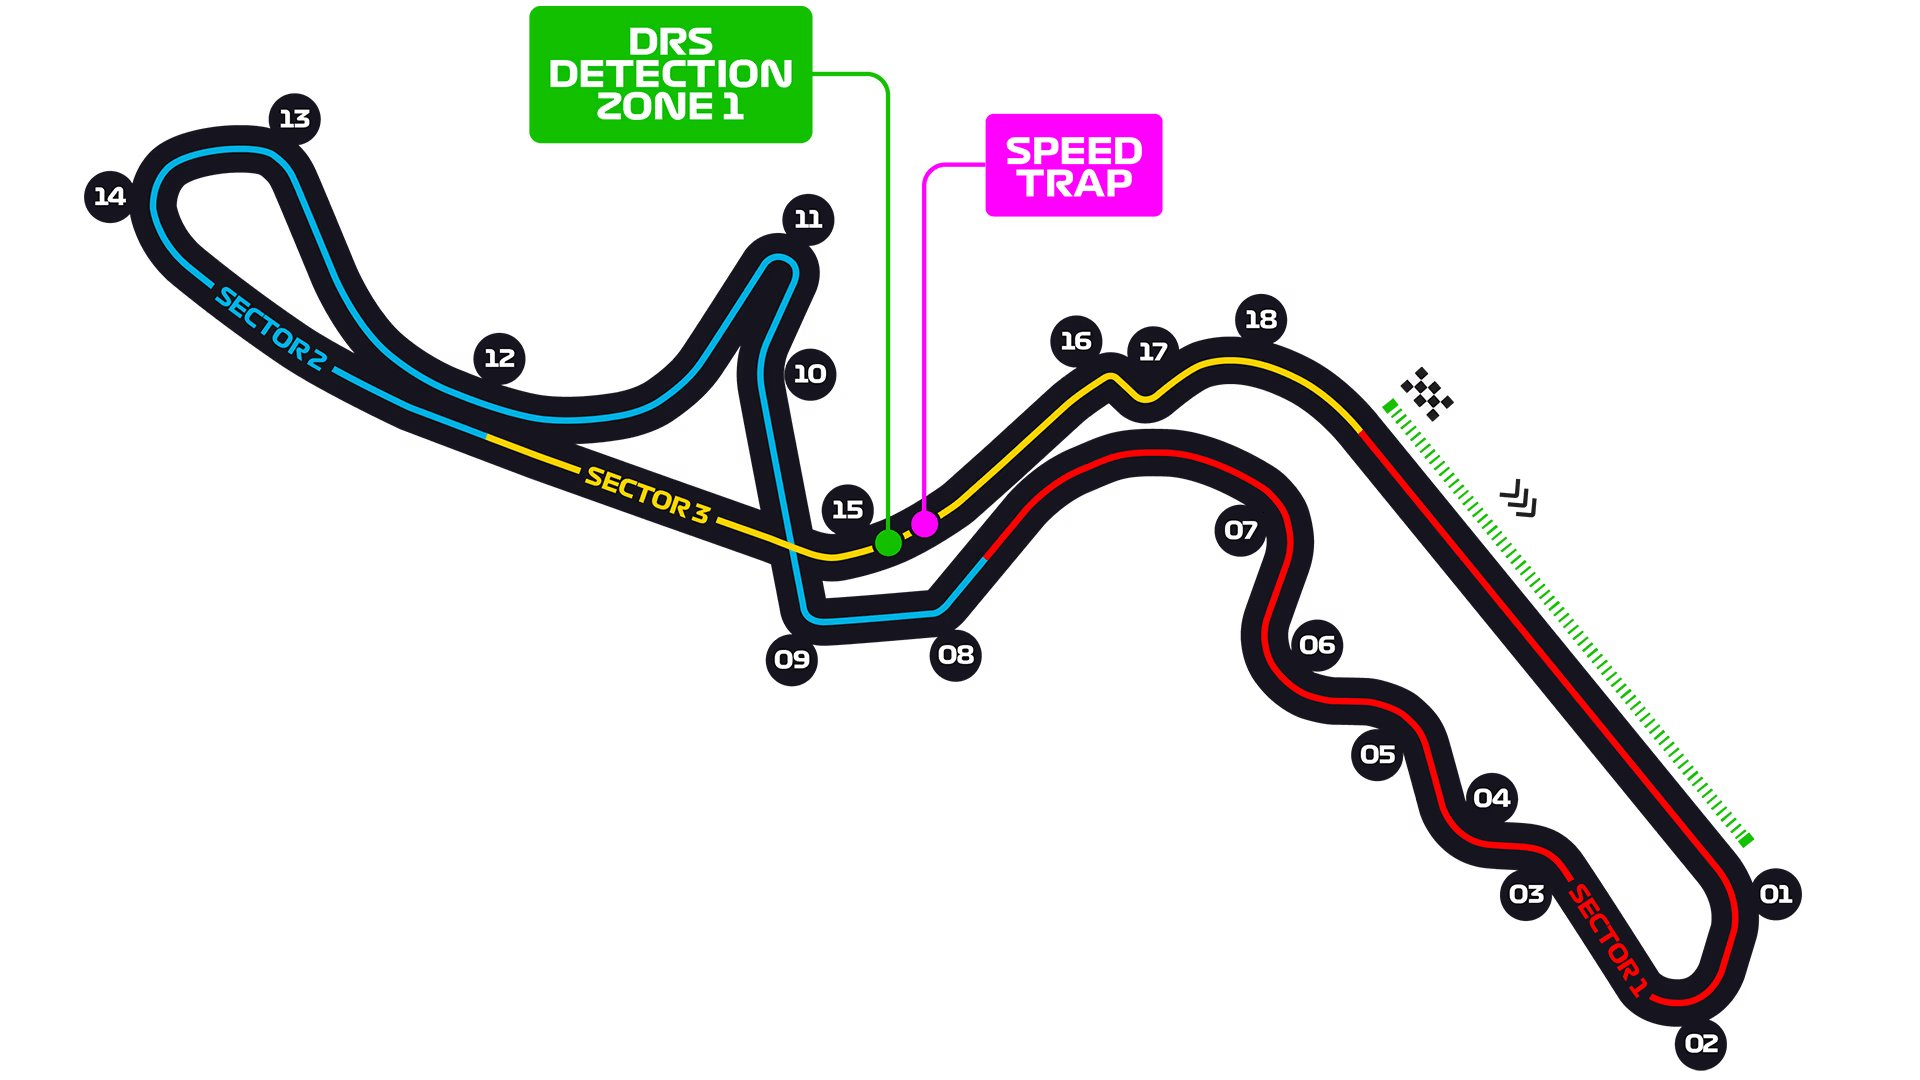
\includegraphics[width=0.75\linewidth]{images/4.Japan_Circuit.jpg}
\end{figure}

\begin{itemize}
    \item \textbf{Lap Record} : 1:28.877 (2023, Max Verstappen - Red Bull).
    
    \item \textbf{Number of Corners \& Key Features} : 18 turns (10 right, 8 left) - Unique figure-of-eight layout featuring a technical S-section, high-speed esses, and elevation changes that test both car stability and driver precision.\\
    Teams opt for high-downforce setups, critical to handle Suzuka’s combination of fast S-curves, technical sections, and lengthy straights. Wind direction notably impacts performance in the high-speed first sector.
    
    \item \textbf{Braking Zones \& Overtaking} : Braking zones such as the entry to the Esses and the hairpin are prime overtaking spots, though passing opportunities are limited overall due to the circuit’s rhythm.
    
    \item \textbf{Tyre Degradation \& Strategy} : High tyre degradation from multiple high-speed, high-downforce corners contributes to the popularity of two-stop strategies.

    \item \textbf{Weather \& Environment} : Suzuka often features variable weather and challenging wind patterns, especially in the S-curves, which can unsettle car balance.
\end{itemize}

\textbf{Strategic Summary :}
Suzuka demands aerodynamic efficiency, mechanical grip, precision, and tyre management. It pushes both car and driver across varying corner types, often resulting in high tyre wear and strategic diversity.


\subsection{Race Analysis}

\textbf{Date:} 7 April 2024 — 14:00 local time 

\begin{itemize}
    \item \textbf{Qualifying Summary} : \textbf{Pole Position:} Max Verstappen (Red Bull) – 1:28.197 (new track record). \\
    Grid: Pérez 2nd, Norris 3rd, Sainz 4th.
    
    \item \textbf{Race Summary} : \textbf{Winner:} Max Verstappen (Red Bull). \\
    \textbf{Podium:} 1. Verstappen - 2. Pérez - 3. Sainz.\\
    \textbf{Notable incidents:} Ricciardo and Albon crashed at Turn 3 (Red flag first lap).
    
    \item \textbf{Strategies} : 
    - Verstappen \& Pérez — two-stop (Medium–Hard–Hard). Managed degradation and pace with clean air.\\
    - Ferrari — Leclerc attempted one-stop (Medium–Hard). Dropped behind Sainz, who was on a two-stop with fresher tyres. \\
    - McLaren — Norris and Piastri on two-stops but lacked long-run pace compared to Ferrari. \\
    - Tsunoda — secured P10 with smart one-stop, scoring points at home.

    \item \textbf{Performance Trends} : \textbf{Red Bull}’s pace advantage was clear, Verstappen untouchable, Pérez comfortably P2. \\
    \textbf{Ferrari} showed the strongest tyre management among the rest, Leclerc making one-stop work while Sainz maximised tyre offset for podium. \\
    \textbf{McLaren} lacked consistency on high-deg circuit, strong over one lap but dropped behind Ferrari in the race. \\
    \textbf{Mercedes} again struggled with balance in high-speed sections, limiting them to minor points. \\
    \textbf{Aston Martin} competitive with Alonso, but faded in race pace relative to McLaren/Ferrari. \\
    Tsunoda delivered \textbf{Racing Bulls}’ best result of the season with home points, maximising strategy execution. 
    
    \item \textbf{Championship Impact} : \textbf{Drivers:} Verstappen 77 points, Pérez 64 (+1), Leclerc 59 (-1).\\
    \textbf{Constructors:} Red Bull 141, Ferrari 120, McLaren 69, Mercedes 34.
\end{itemize}


\subsection{Link \& Takeaway}

\begin{itemize}
    \item The high-downforce, high-tyre-demand nature of Suzuka played into the hands of teams who balanced durability with speed. Red Bull’s ability to extract tyre life and maintain pace under pressure proved decisive.
    \item Ferrari’s one-stop strategy, hinging on Leclerc’s medium-to-hard transition, showcased smart adaptation to the circuit’s degradation traits, even if ultimately insufficient to beat Red Bull’s pace.
    \item McLaren competitive in qualifying but dropped back in race pace — highlighting limits in high-degradation scenarios. 
    \item Mercedes struggled with balance and traction out of slow zones, limiting them to minor points. 
    \item Tsunoda’s home points finish underlined both his maturity and Racing Bulls’ ability to capitalise on attrition.
\end{itemize}
\section{Chinese Grand Prix}

\subsection{Circuit Analysis}

\textbf{Circuit Name:} Shanghai International Circuit (Shanghai, China) \\
\textbf{Length:} 5.451 km - \textbf{Laps:} 56 - \textbf{Total Distance:} 305.066 km

\begin{figure}[H]
    \centering
    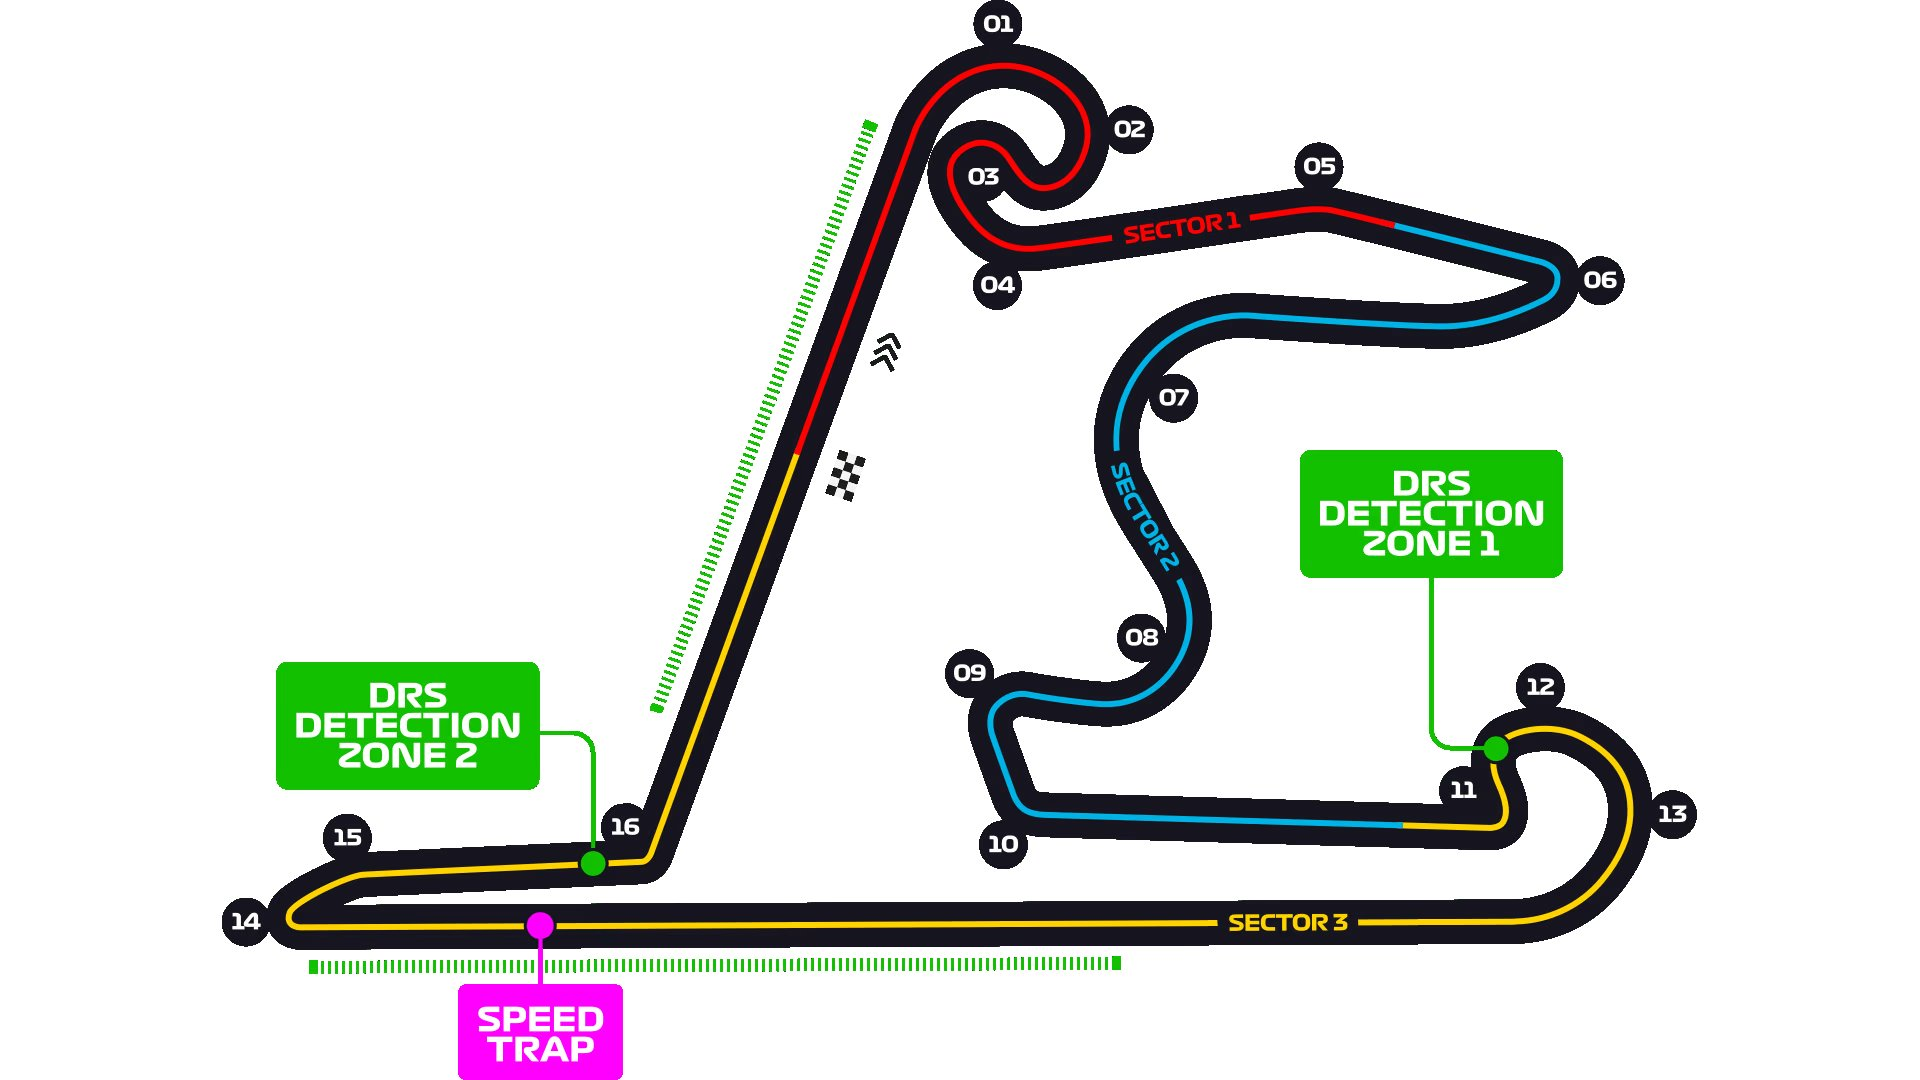
\includegraphics[width=0.75\linewidth]{images/5.China_Circuit.jpg}
\end{figure}

\begin{itemize}
    \item \textbf{Lap Record} : 1:31.095 (2018, Sebastian Vettel – Ferrari).

    \item \textbf{Number of Corners \& Key Features} : 16 turns (9 right, 7 left). \\
    Famous opening complex (Turns 1–2) with a tightening radius, long back straight (1.2 km) leading to heavy braking at Turn 14. \\
    Mix of high-speed esses (Turns 7–8) and slow technical corners (Turn 6, Turn 11).

    \item \textbf{Braking Zones \& Traction} : Major braking at Turn 14 (down from ~330 km/h to 70 km/h). \\
    Traction is critical exiting Turns 6, 13 and 14 due to long acceleration phases.

    \item \textbf{DRS \& Overtaking} : Two DRS zones (start/finish straight, long back straight). \\
    Turn 14 is the prime overtaking zone, Turn 6 also offers chances.

    \item \textbf{Tyre Degradation \& Strategy} : Front-left tyre wear is a known issue due to long right-handers. \\
    Most teams targeted two-stop strategies, but one-stop possible with tyre management.

    \item \textbf{Weather \& Environment} : Cool spring conditions, track temp lower than Middle East races. \\
    Wind and smog sometimes affect visibility and downforce balance.
\end{itemize}

\textbf{Strategic Summary :}  
Shanghai demands strong aerodynamic efficiency for the high-speed esses and mechanical grip for the slow hairpins. The long back straight rewards power units and top speed, while tyre wear (front-left) requires careful management. Strategy flexibility (1–2 stops) is crucial depending on tyre degradation.

\subsection{Race Analysis}

\textbf{Date:} Sprint : 20 April 2024 - 11:00 local time\\
Race : 21 April 2024 — 15:00 local time 

\begin{itemize}
    \item \textbf{Sprint Qualifying:} \textbf{Pole Position:} Lando Norris (McLaren) - 1:57.940.\\
    Grid : Hamilton 2nd, Alonso 3rd, Verstappen 4th.

    \item \textbf{Sprint Summary} : \textbf{Winner:} Max Verstappen (Red Bull). \\
    \textbf{Podium}: 1. Verstappen - 2. Hamilton - 3. Pérez. \\
    Norris, who started from pole, went wide Lap 1 and fell to P6.\\
    Alonso (10s penalty) retired after contact with Sainz.

    \item \textbf{Qualifying Summary} : \textbf{Pole Position:} Max Verstappen (Red Bull) - 1:33.660. \\
    Grid: Pérez 2nd, Alonso 3rd, Norris 4th.\\

    \item \textbf{Race Summary} : \textbf{Winner:} Max Verstappen (Red Bull) — dominant pace, controlled from the front. \\
    \textbf{Podium:} 1. Verstappen - 2. Norris - 3. Pérez . \\
    Alonso, after starting P3, faded with tyre wear and ended P7 but took fastest lap.\\
    \textbf{Technical issues:} Bottas (engine - Virtual Safety Car lap 20).\\
    \textbf{Notable incidents:} Ricciardo crashed because of Stroll (10s penalty) + Tsunoda crashed because of Magnusssen (10s penalty) (Safety Car lap 26).

    \item \textbf{Strategies} : Most drivers adopted a two-stop race due to heavy front-left degradation. \\
    - Red Bull ran Soft–Hard–Medium, Verstappen extending his middle stint to stay in control even after the Safety Car. \\
    - Norris benefited from a perfectly timed stop under VSC on lap 20, which allowed him to jump Alonso and challenge Pérez. \\
    - Ferrari committed to a standard two-stop plan but suffered graining on the Mediums, which limited their race pace. \\
    - Mercedes split approaches: Russell on Soft–Medium–Hard, while Hamilton started from P18 with a more aggressive Soft–Medium–Medium that helped him recover to P9. \\
    - Alonso attempted a three-stop strategy to mitigate tyre wear. Although it cost him track position, he secured the fastest lap in the closing stages. \\

    \item \textbf{Performance Trends} : \textbf{Red Bull} — Verstappen dominant (led 51/56 laps), Pérez solid P3. Car excelled in traction + straights.\\
    \textbf{McLaren} — Norris capitalised on SC timing, excellent straight-line speed, secured P2 and Driver of the Day.\\
    \textbf{Ferrari} — Leclerc P4, Sainz P5. Tyre degradation (front-left graining) limited their challenge.\\
    \textbf{Mercedes} — Russell P6 consistent, Hamilton recovered from P18 to P9.

    \item \textbf{Championship Impact} : \textbf{Drivers:} Verstappen 110 points, Pérez 85, Leclerc 76.\\
    \textbf{Constructors:} Red Bull 195, Ferrari 151, McLaren 96, Mercedes 52.
\end{itemize}

\textbf{Key Takeaway :}  
Red Bull confirmed their superiority on a mixed circuit layout, Verstappen flawless from pole. McLaren proved highly competitive on power-sensitive tracks, while Ferrari’s tyre weakness cost them.

\subsection{Link \& Takeaway}

\begin{itemize}
    \item Shanghai’s long straights and heavy braking zones rewarded Red Bull’s traction and straight-line speed.
    \item Norris and McLaren capitalised on their efficiency to secure P2, confirming progress on power tracks.
    \item Ferrari’s tyre degradation issues (front-left wear) matched circuit expectations and limited their challenge.
    \item Safety Car and penalties affected midfield but not the Verstappen-led top order, showing how dominant Red Bull remained.
    \item Alonso’s fastest lap underlined Aston Martin’s potential on fresh tyres but highlighted lack of long-run race pace.
\end{itemize}

\section{Miami Grand prix}

\subsection{Circuit Analysis}

\textbf{Circuit Name:} Miami International Autodrome (Miami, USA) \\
\textbf{Length:} 5.412 km - \textbf{Laps:} 57 - \textbf{Total Distance:} 308.326 km

\begin{figure}[H]
    \centering
    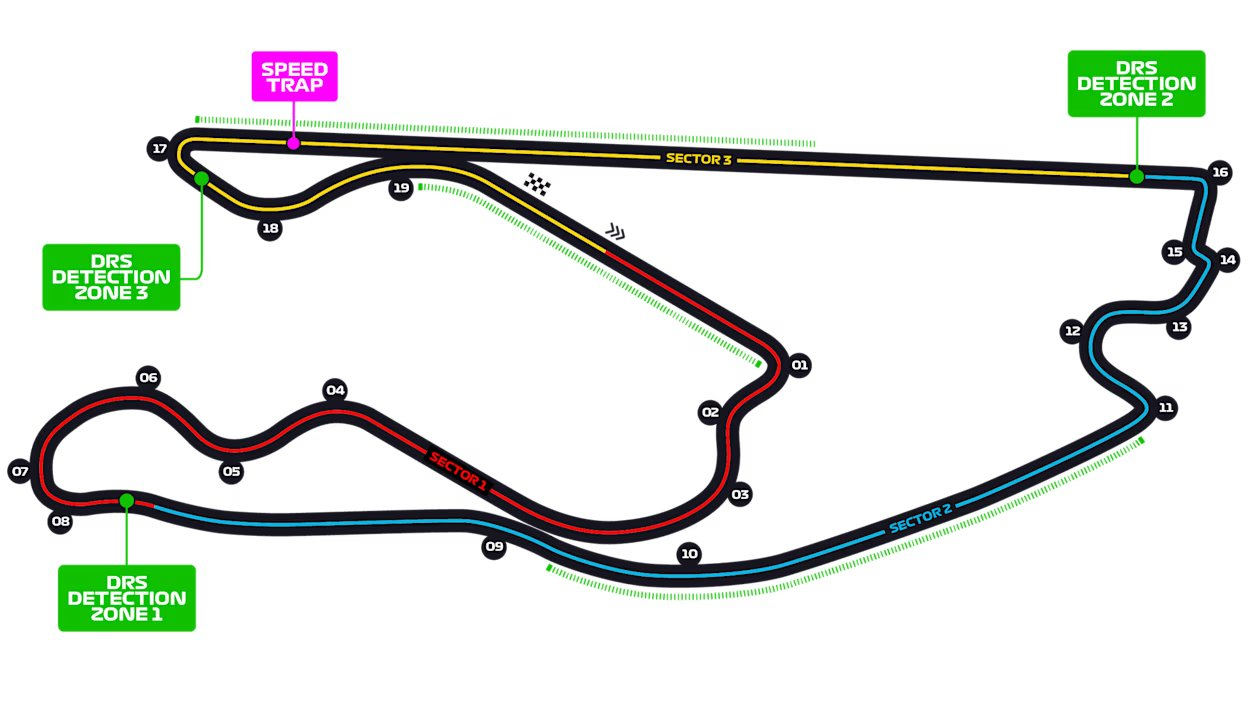
\includegraphics[width=0.75\linewidth]{images/6.Miami_Circuit.jpg}
\end{figure}

\begin{itemize}
    \item \textbf{Lap Record} : 1:26.841 (2023, Sergio Pérez - Red Bull).
    
    \item \textbf{Number of Corners \& Key Features} : 19 turns (7 right, 12 left) - Combination of fast sections (Turns 4–8), long back straight into heavy braking at Turn 17, and a tight, technical complex between Turns 11–16.
    
    \item \textbf{Braking Zones \& Traction} : Heavy braking at Turn 17 (from ~320 km/h down to 70 km/h). Traction crucial out of Turn 16 leading onto the long straight.
    
    \item \textbf{DRS \& Overtaking} : Three DRS zones (between Turns 9–11, 16–17, and main straight). Best overtaking chances at Turn 11 and Turn 17.
    
    \item \textbf{Tyre Degradation \& Strategy} : Tyre wear relatively low but thermal degradation high due to heat. \\
    One-stop strategies favoured, though Safety Cars can shuffle plans.
    
    \item \textbf{Weather \& Environment} : Hot and humid conditions typical of Miami in May.\\
    Track surface is new and evolving, often slippery off-line.\\
    Risk of thunderstorms and high humidity affects grip and cooling.
\end{itemize}

\textbf{Strategic Summary :}
Miami rewards cars with high straight-line speed and braking stability, while the technical sector demands strong low-speed traction. Tyre management and cooling are critical due to high ambient temperatures. Safety Cars are common and can be decisive.


\subsection{Race Analysis}

\textbf{Date:} Sprint : 4 May 2024 - 12:00 local time\\
Race : 5 May 2024 — 16:00 local time 

\begin{itemize}
    \item \textbf{Sprint Qualifying:} \textbf{Pole Position:} Max Verstappen (Red Bull) - 1:27.641.\\
    Grid : Leclerc 2nd, Pérez 3rd, Ricciardo 4th.

    \item \textbf{Sprint Summary} : \textbf{Winner:} Max Verstappen (Red Bull). \\
    \textbf{Podium}: 1. Verstappen - 2. Leclerc - 3. Pérez. \\
    Hamilton triggered contact at Turn 1 (+ 20s) → Alonso + Stroll caught out, Norris spun and retired.\\
    Ricciardo finished P4, Tsunoda scored P8. 
    
    \item \textbf{Qualifying Summary} : \textbf{Pole Position:} Max Verstappen (Red Bull) – 1:27.241. \\
    Grid: Leclerc 2nd, Sainz 3rd, Pérez 4th.
    
    \item \textbf{Race Summary} : \textbf{Winner:} Lando Norris (McLaren) - his first F1 victory\\
    \textbf{Podium:} 1. Norris - 2. Verstappen - 3. Leclerc.\\
    \textbf{Technical issues:} Hamilton (damage after early contact, retired lap 33).
    \textbf{Notable incidents:} Safety Car on lap 29 after Kevin Magnussen and Logan Sargeant collided, which allowed Norris to pit at the perfect time and undercut Verstappen.
    
    \item \textbf{Strategies} : Majority opted for one-stop.\\
    - Verstappen started on mediums then switched to hards (standard plan). \\
    - Norris benefited from pitting under the Safety Car (Medium–Hard with track position gain).\\
    - Ferrari followed conservative Medium–Hard but lacked late pace.
    
    \item \textbf{Performance Trends} : \textbf{McLaren} — Major upgrades transformed pace. Norris flawless, Piastri unlucky with contact.\\
    \textbf{Red Bull} — Verstappen still dominant in pace, but strategy luck beat him. Pérez only P4.\\
    \textbf{Ferrari} — Strong consistency: Leclerc on podium, Sainz P5.\\
    \textbf{Mercedes} — Decent recovery, solid points but off the front-running pace.\\
    \textbf{Midfield} — Tsunoda shined P7. Alonso salvaged P9 despite weak weekend. Ocon scored Alpine’s first point of 2024.
    
    \item \textbf{Championship Impact} : \textbf{Drivers:} Verstappen 136 points, Pérez 103, Leclerc 98.\\
    \textbf{Constructors:} Red Bull 239, Ferrari 187, McLaren 124, Mercedes 64.    
\end{itemize}

\textbf{Key Takeaway :}
Norris and McLaren seized their moment, perfectly exploiting the Safety Car. Red Bull remained the benchmark in raw pace, but Miami proved strategy and timing can beat outright speed.


\subsection{Link \& Takeaway}

\begin{itemize}
    \item Miami’s long straights and heavy braking zones usually favour Red Bull, but the Safety Car timing flipped the race. 
    \item Ferrari showed consistency but lacked outright pace to fight for the win.
    \item Miami’s Safety Car timing completely reshuffled the order, benefiting Norris. 
    \item McLaren’s upgrades paid off instantly, transforming potential into a breakthrough win. 
    \item Alpine finally scored points. Tsunoda and Racing Bulls continued strong midfield form.
\end{itemize}
\section{Emilia-Romagna Grand prix}

\subsection{Circuit Analysis}

\textbf{Circuit Name:} Autodromo Enzo e Dino Ferrari (Imola, Italy) \\
\textbf{Length:} 4.909 km - \textbf{Laps:} 63 - \textbf{Total Distance:} 309.049 km

\begin{figure}[H]
    \centering
    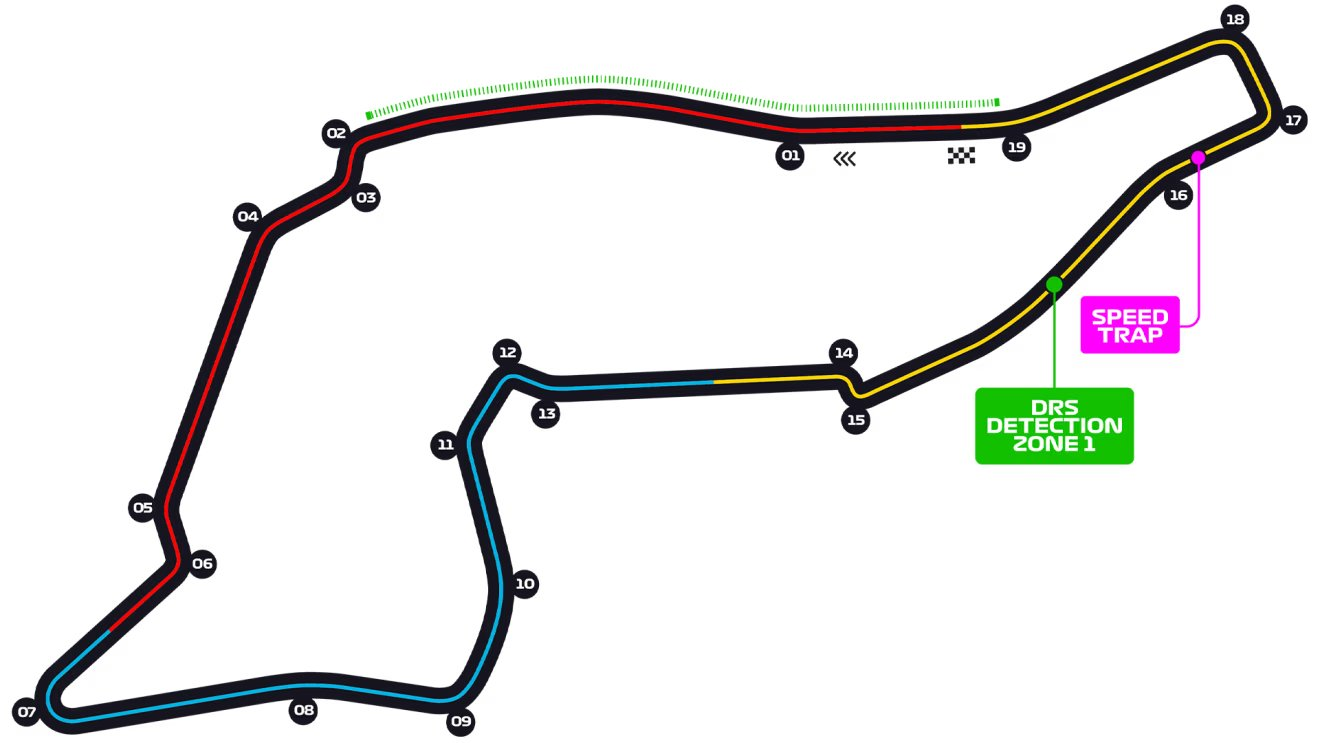
\includegraphics[width=0.75\linewidth]{images/7.Emilia_Romagna_Circuit.jpg}
\end{figure}

\begin{itemize}
    \item \textbf{Lap Record} : 1:13.609 (2020, Valtteri Bottas - Mercedes).
    
    \item \textbf{Number of Corners \& Key Features} : 19 turns (9 right, 10 left)
    
    \item \textbf{Braking Zones \& Traction} : Heavy braking at Variante Alta and Turn 1 chicane.\\
    Strong traction required exiting Rivazza onto the main straight.
    
    \item \textbf{DRS \& Overtaking} : Single DRS zone along the main straight. Overtaking possible at Turn 2 (Tamburello) after the DRS, but otherwise limited.
    
    \item \textbf{Tyre Degradation \& Strategy} : Tyre wear moderate, a one-stop Medium–Hard is the preferred strategy.\\
    Track position critical due to limited overtaking.
    
    \item \textbf{Weather \& Environment} : Spring in Emilia-Romagna brings variable conditions, risk of rain often present. Track is narrow with little runoff, making mistakes costly.
\end{itemize}

\textbf{Strategic Summary :}
Imola emphasises track position, consistency, and precision. Qualifying is vital, as overtaking is difficult. One-stop strategies are common, but Safety Cars can create opportunities.


\subsection{Race Analysis}

\textbf{Date:} 19 May 2024 — 15:00 local time 

\begin{itemize}
    \item \textbf{Qualifying Summary} : \textbf{Pole Position:} Max Verstappen (Red Bull) – 1:14.746. \\
    Grid: Norris 2nd, Leclerc 3rd, Sainz 4th.
    Oscar Piastri, who finished 2nd during the qualifications, was penalised of three grid places for impeding.
    
    \item \textbf{Race Summary} : \textbf{Winner:} Max Verstappen (Red Bull).\\
    \textbf{Podium:} 1. Verstappen - 2. Norris - 3. Leclerc.\\
    \textbf{Technical issues:} Sainz (overheating, struggled all race).\\
    Verstappen led most of the race but struggled with tyre wear late on. Norris closed the gap to 0.7s at the finish, but DRS wasn’t enough to force a pass. Leclerc consistent in P3. \\
    Sainz faded with overheating and was undercut by Piastri for P4. Mercedes steady in P6–P7. Pérez only P8, struggling in traffic.
    
    \item \textbf{Strategies} : Majority followed Medium–Hard one-stop strategy.\\
    - Norris attempted an undercut but was held in traffic, losing crucial time. \\
    - Verstappen stopped early to cover Norris.\\
    - Ferrari also on Medium–Hard but Leclerc lacked the pace to challenge McLaren.
    
    \item \textbf{Performance Trends} :\textbf{Red Bull} — Still strongest in qualifying and defending track position, but tyre wear was an issue late in stints. 
    \textbf{McLaren} — Norris showed real pace and tyre conservation, only limited by traffic and overtaking difficulty. 
    \textbf{Ferrari} — Consistent podium pace, but lacked the raw speed to pressure Red Bull and McLaren. 
    \textbf{Mercedes} — Solid points but a step behind. Russell’s fastest lap masked underlying lack of pace.
    
    \item \textbf{Championship Impact} : \textbf{Drivers:} Verstappen 161 points, Leclerc 113 (+1), Pérez 107 (-1).\\
    \textbf{Constructors:} Red Bull 268, Ferrari 212, McLaren 154, Mercedes 79.    
\end{itemize}

\textbf{Key Takeaway :}
Verstappen’s defensive driving under pressure secured victory. McLaren confirmed their rise with Norris pushing Verstappen to the limit. Ferrari solid but lacked enough speed to fight for the win at home.


\subsection{Link \& Takeaway}

\begin{itemize}
    \item Imola’s narrow layout and lack of overtaking rewarded Verstappen’s pole and strong defence.  
    \item Norris and McLaren showed they could pressure Red Bull on pure pace, but traffic in pit strategy denied them a shot at victory.
    \item Ferrari’s limitations in long-run pace were exposed on home soil, despite Leclerc’s podium. 
    \item Track position proved decisive, underlining Imola’s strategic rigidity.
\end{itemize}
\section{Monaco Grand prix}

\subsection{Circuit Analysis}

\textbf{Circuit Name:} Circuit de Monaco (Monte Carlo, Monaco) \\
\textbf{Length:} 3.337 km - \textbf{Laps:} 78 - \textbf{Total Distance:} 260.286 km

\begin{figure}[H]
    \centering
    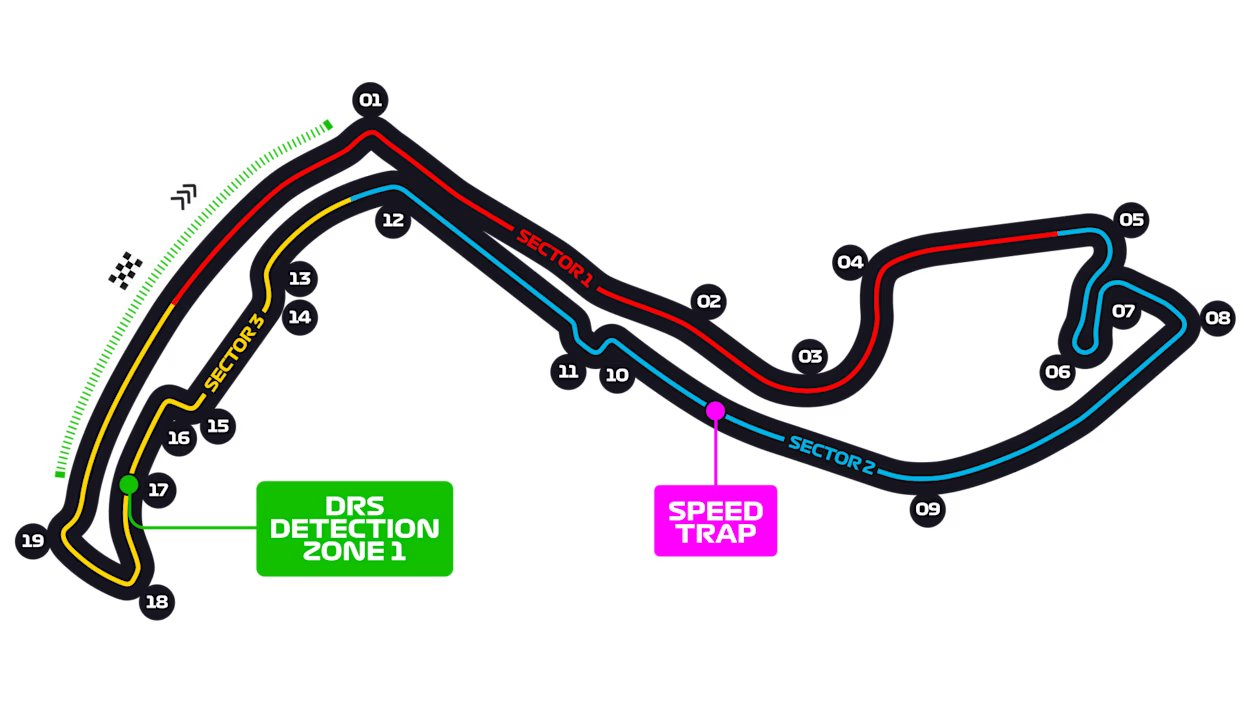
\includegraphics[width=0.75\linewidth]{images/8.Monaco_Circuit.jpg}
\end{figure}

\begin{itemize}
    \item \textbf{Lap Record} : 1:10.166 (2019, Lewis Hamilton – Mercedes).
    
    \item \textbf{Number of Corners \& Key Features} : 19 turns (11 right, 8 left) - Iconic layout through the streets of Monte Carlo, featuring tight hairpins (Grand Hotel Hairpin), fast tunnel section, and narrow barriers throughout.
    
    \item \textbf{Braking Zones \& Traction} : Major braking at Sainte Dévote (Turn 1), Mirabeau, and the Nouvelle Chicane. Traction critical out of the hairpin and Portier leading into the tunnel.
    
    \item \textbf{DRS \& Overtaking} : Single DRS zone along the main straight.\\
    Overtaking extremely limited, pit strategy and track position are decisive.
    
    \item \textbf{Tyre Degradation \& Strategy} : Tyre wear generally low, but graining can occur on softs.\\
    Most teams opted for one-stop, with pit timing more important than degradation.
    
    \item \textbf{Weather \& Environment} : Coastal location brings variable conditions, rain often change strategy. Narrow barriers punish even minor mistakes.
\end{itemize}

\textbf{Strategic Summary :}
Monaco rewards qualifying performance and flawless execution. Overtaking is almost impossible, so grid position and pit-stop timing are critical. Drivers must balance precision with risk around the unforgiving barriers.


\subsection{Race Analysis}

\textbf{Date:} 26 May 2024 — 15:00 local time 

\begin{itemize}
    \item \textbf{Qualifying Summary} : \textbf{Pole Position:} Charles Leclerc (Ferrari) – 1:10.270. \\
    Grid: Piastri 2nd, Sainz 3rd, Norris 4th.\\
    Verstappen only P6 after struggling in Q3.
    
    \item \textbf{Race Summary} : \textbf{Winner:} Charles Leclerc (Ferrari) - his first home victory.\\
    \textbf{Podium:} 1. Leclerc - 2. Piastri - 3. Sainz.\\
    \textbf{Notable incidents:} 
    - Perez and Magnussen collided on lap 1, both retired (red flag).\\
    - Ocon crashed into teammate Gasly at Portier, retired + 5-place grid penalty for Canada.
    
    \item \textbf{Strategies} : 
    - Red flag lap 1 allowed teams to switch tyres freely → most locked into a one-stop equivalent.\\ 
    - Leclerc controlled race on hard tyres, perfectly managing pace to keep Piastri behind. \\
    - Sainz strategically slowed Norris to avoid undercut threats from Russell. \\
    - Hamilton + Verstappen pitted late for fresh tyres to chase fastest lap → Hamilton succeeded on lap 63.
    
    \item \textbf{Performance Trends} : \textbf{Ferrari} delivered both one-lap speed and flawless race execution. Leclerc never relinquished the lead across 78 laps. \\
    \textbf{McLaren} continued strong form, Piastri competitive throughout, Norris closely behind. \\
    \textbf{Mercedes} solid but unspectacular — Russell P5, Hamilton P7 + fastest lap bonus. \\
    \textbf{Red Bull} struggled badly with setup and traction. Verstappen stuck in P6 all race, Pérez out on lap 1. \\
    \textbf{Tsunoda} consistent and secured more points for Racing Bulls. \\
    \textbf{Williams} scored their first points of the season with Albon P9. \\
    \textbf{Alpine} endured intra-team chaos. Gasly salvaged P10, Ocon retired lap 1. \\
    
    \item \textbf{Championship Impact} : \textbf{Drivers:} Verstappen 169 points, Leclerc 138, Norris 113 (+1).\\
    \textbf{Constructors:} Red Bull 276, Ferrari 252, McLaren 184, Mercedes 96.    
\end{itemize}

\textbf{Key Takeaway :}
Verstappen’s defensive driving under pressure secured victory. McLaren confirmed their rise with Norris pushing Verstappen to the limit. Ferrari solid but lacked enough speed to fight for the win at home.


\subsection{Link \& Takeaway}

\begin{itemize}
    \item Monaco once again proved the near impossibility of overtaking, qualifying dictated the race outcome. 
    \item The early red flag simplified strategies into an early one-stop, making overtaking virtually impossible.
    \item Ferrari capitalised perfectly on their one-lap advantage, securing both pace and control. 
    \item McLaren confirmed themselves as Ferrari’s closest challengers on high-downforce circuits. 
    \item Red Bull looked unusually vulnerable, with Verstappen unable to advance and Pérez eliminated lap 1. 
    \item Mercedes secured solid points but remain distant from Ferrari/McLaren pace. 
\end{itemize}
\section{Canadian Grand prix}

\subsection{Circuit Analysis}

\textbf{Circuit Name:} Circuit Gilles-Villeneuve (Montréal, Canada) \\
\textbf{Length:} 4.361 km - \textbf{Laps:} 70 - \textbf{Total Distance:} 305.270 km

\begin{figure}[H]
    \centering
    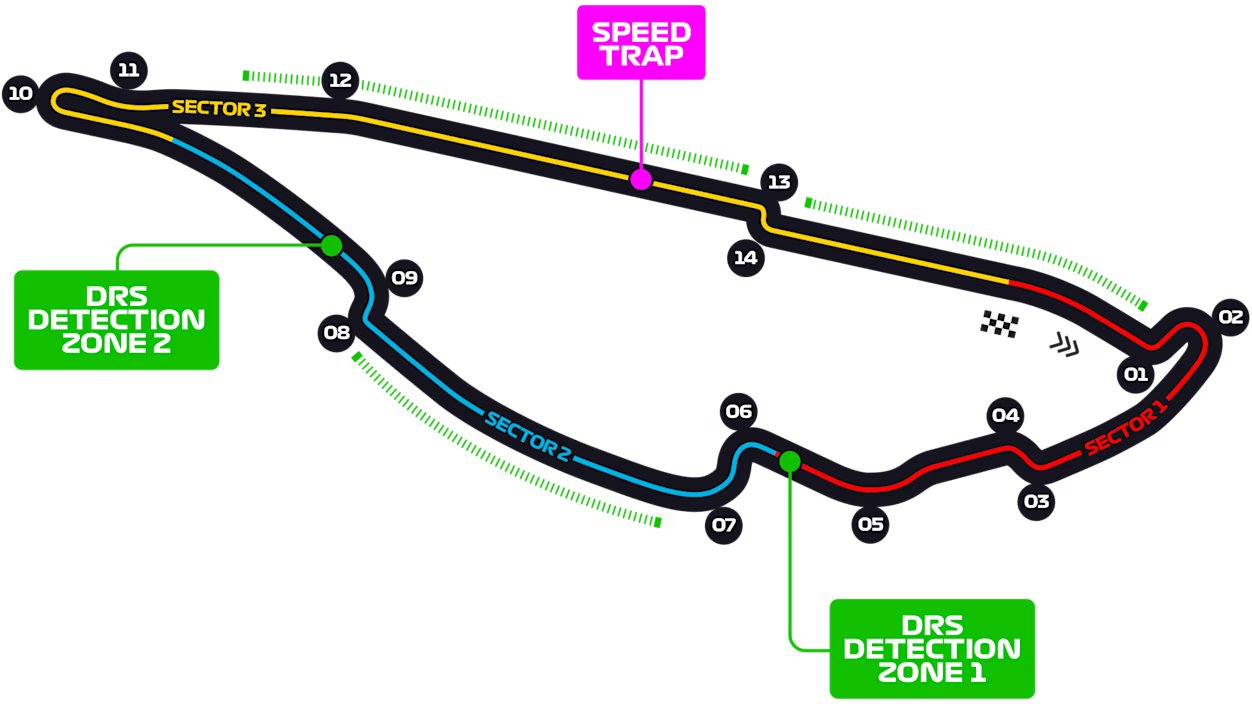
\includegraphics[width=0.75\linewidth]{images/9.Canada_Circuit.jpg}
\end{figure}

\begin{itemize}
    \item \textbf{Lap Record} : 1:10.240 (2019, Sebastian Vettel – Ferrari).
    
    \item \textbf{Number of Corners \& Key Features} : 13 turns (8 right, 5 left) - Semi-permanent circuit on Notre Dame Island. Famous for the “Wall of Champions” at the final chicane. Mix of long straights and heavy braking chicanes, rewarding top speed and strong traction.
    
    \item \textbf{Braking Zones \& Traction} : Heavy braking into Turns 1, 10 (L’Epingle hairpin), and the final chicane. Traction is crucial out of Turn 10 onto the long Casino Straight.
    
    \item \textbf{DRS \& Overtaking} : Three DRS zones (start/finish straight, Casino Straight, between Turns 7–8). \\
    Prime overtaking spots at the hairpin (T10) and into the final chicane.
    
    \item \textbf{Tyre Degradation \& Strategy} : Tyre degradation usually low, but graining possible in cool or damp conditions. \\
    One-stop strategies possible, though Safety Cars often change plans.
    
    \item \textbf{Weather \& Environment} : Early summer weather is unpredictable, frequent risk of rain. \\
    Cooler temps increase risk of graining. \\
    Safety Car probability high due to walls and narrow runoff.
\end{itemize}

\textbf{Strategic Summary :}
Montréal rewards power units, braking stability, and traction. Track position is important but overtaking is more feasible than Monaco or Imola. Strategy must remain flexible due to high chance of Safety Car or weather disruption.


\subsection{Race Analysis}

\textbf{Date:} 9 June 2024 — 14:00 local time 

\begin{itemize}
    \item \textbf{Qualifying Summary} : \textbf{Pole Position:} George Russell (Mercedes) – 1:12.000 - (equal to Verstappen, Russell ahead by setting time first). \\
    Grid: Verstappen 2nd, Norris 3rd, Piastri 4th.\\
    Leclerc and Sainz started from the midfield after poor qualifying.
    
    \item \textbf{Race Summary} : \textbf{Winner:} Max Verstappen (Red Bull).\\
    \textbf{Podium:} 1. Verstappen - 2. Norris - 3. Russell.\\
    \textbf{Technical issues:} Leclerc (power unit).\\
    \textbf{Notable incidents:} Multiple Safety Cars — including one on lap 54 after Sainz’s crash at Turn 6.
    
    \item \textbf{Strategies} : Most teams switched between slicks and intermediates.\\
    - Verstappen timed pit stops perfectly (under Safety Car), maintaining track position.\\ 
    - Norris lost victory chance due to unlucky Safety Car timing. 
    - Mercedes split strategies, Russell and Hamilton both strong on mediums late. 
    Alpine executed perfectly, double points finish from deep in the grid.
    
    \item \textbf{Performance Trends} : \textbf{Red Bull:} proved adaptable in mixed weather, Verstappen perfect under pressure.
    \textbf{McLaren:} Norris fastest in race conditions, unlucky with SC. Piastri competitive but edged by Mercedes. 
    \textbf{Mercedes:} Best weekend of 2024 so far, Russell pole + podium, Hamilton fastest lap and P4. 
    \textbf{Ferrari:} Disaster: poor quali, Leclerc PU failure, Sainz crash. Big blow in championship. 
    \textbf{Aston Martin:} Strong, Alonso P6, Stroll P7 at home GP. 
    \textbf{Racing Bulls:} Ricciardo excellent (Qualified P5, P8 despite penalty), Tsunoda error-strewn (P14). 
    \textbf{Alpine:} Best weekend so far, Gasly P9, Ocon P10, both in points. 
    \textbf{Haas:} Great opening laps on wets, but faded to P11–12.
    
    \item \textbf{Championship Impact} : \textbf{Drivers:} Verstappen 194 points, Leclerc 138, Norris 131.\\
    \textbf{Constructors:} Red Bull 301, Ferrari 252, McLaren 212, Mercedes 124.    
\end{itemize}

\textbf{Key Takeaway :}
Verstappen thrived in chaos, securing another win in a rain-affected race. McLaren continued their strong momentum, while Mercedes finally showed flashes of competitiveness. Ferrari’s double DNF dealt a huge blow to their title hopes.


\subsection{Link \& Takeaway}

\begin{itemize}
    \item The high Safety Car probability at Montréal struck again, timing was decisive, costing Norris and saving Verstappen. 
    \item Ferrari’s failure exposed their fragility: from consistency to a double DNF. 
    \item Mercedes took a genuine step forward, showing both one-lap and race pace. 
    \item McLaren confirmed they are now Red Bull’s closest rivals. 
    \item Alpine finally delivered a clean weekend and double points. 
    \item Aston Martin secured much-needed points with both drivers, stabilising their season. 
\end{itemize}
\section{Spanish Grand prix}

\subsection{Circuit Analysis}

\textbf{Circuit Name:} Circuit de Barcelona-Catalunya (Montmeló, Spain) \\
\textbf{Length:} 4.657 km - \textbf{Laps:} 66 - \textbf{Total Distance:} 307.236 km

\begin{figure}[H]
    \centering
    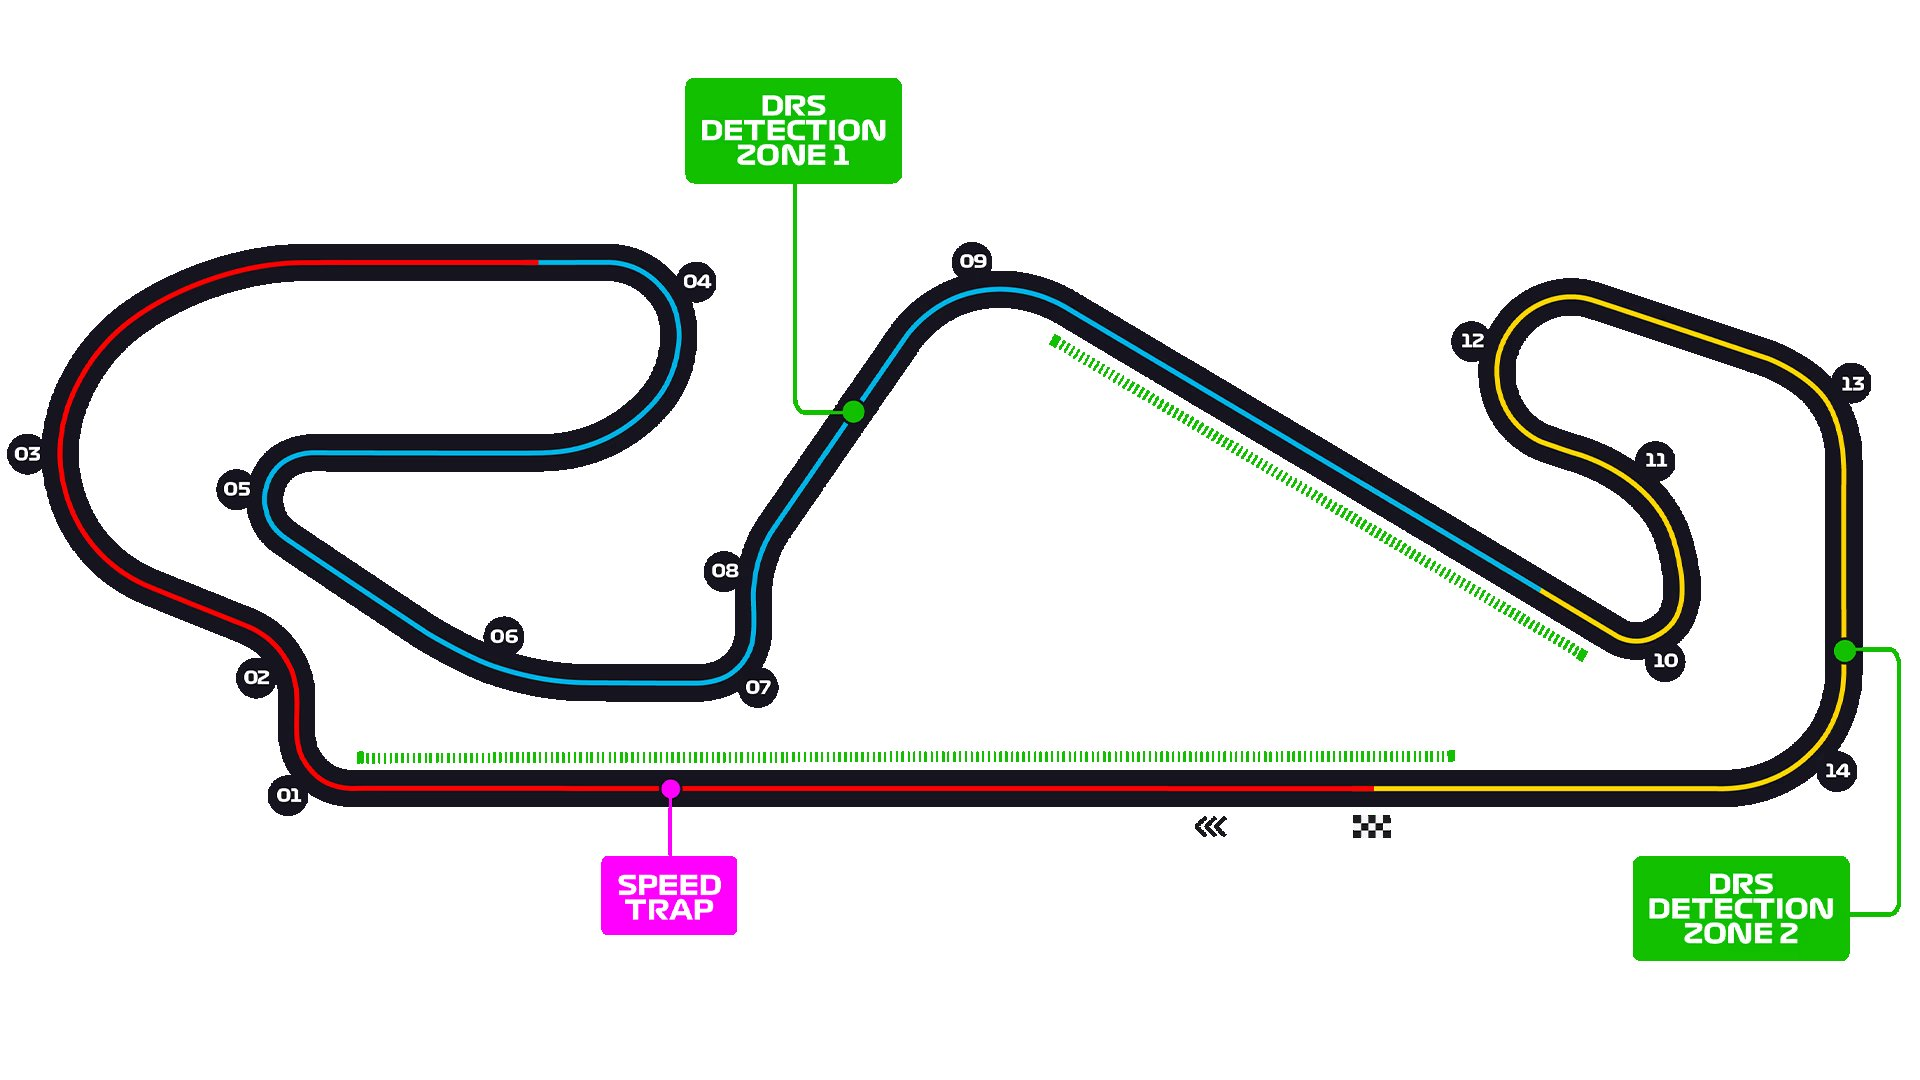
\includegraphics[width=0.75\linewidth]{images/10.Spain_Circuit.jpg}
\end{figure}

\begin{itemize}
    \item \textbf{Lap Record} : 1:12.272 (2023, Max Verstappen - Red Bull).
    
    \item \textbf{Number of Corners \& Key Features} : 14 turns (8 right, 6 left) - Known for its mix of high-, medium-, and low-speed corners, including long Turn 3 and quick Turn 9 (Campsa). Final sector technical, requiring high downforce.
    
    \item \textbf{Braking Zones \& Traction} : Heavy braking at Turn 1 (first chicane) and Turn 10 (La Caixa). Good traction needed out of the final corner onto the main straight.
    
    \item \textbf{DRS \& Overtaking} : Two DRS zones (main straight, between Turns 9–10).\\
    Best overtaking into Turn 1 and Turn 10, though turbulence still makes overtaking challenging.
    
    \item \textbf{Tyre Degradation \& Strategy} : Circuit is abrasive and demanding on tyres, especially front-left.\\
    Two-stop strategies are the norm, tyre management is crucial in hot Spanish conditions.
    
    \item \textbf{Weather \& Environment} : Typically hot and sunny in June, with track temps exceeding 40°C. Wind direction in Turn 3 and Turn 9 often impacts car stability.
\end{itemize}

\textbf{Strategic Summary :}
Barcelona tests overall car performance balance, aero efficiency, tyre management, and downforce. A benchmark track where the fastest car usually wins, but strategy execution remains key.


\subsection{Race Analysis}

\textbf{Date:} 23 June 2024 — 15:00 local time 

\begin{itemize}
    \item \textbf{Qualifying Summary} : \textbf{Pole Position:} Lando Norris (McLaren) – 1:11.383 (new track record). \\
    Grid: Verstappen 2nd, Hamilton 3rd, Russell 4th.\\
    Ferrari struggled for single-lap pace, starting behind Mercedes.
    
    \item \textbf{Race Summary} : \textbf{Winner:} Max Verstappen (Red Bull).\\
    \textbf{Podium:} 1. Verstappen - 2. Norris - 3. Hamilton.
    
    \item \textbf{Strategies} : Standard two-stop race (Medium–Hard–Medium or Medium–Medium–Hard).\\ 
     - Verstappen executed undercut perfectly on Norris at first stop. \\
     - Norris extended his first stint but couldn’t regain track position. \\
     - Mercedes split strategies, Hamilton’s tyre life gave podium edge. \\
     - Ferrari mirrored top strategies but lacked outright pace.\\
    
    \item \textbf{Performance Trends} : \textbf{Red Bull:} Verstappen not dominant by huge margin but managed lead with control. Pérez again underwhelming in P8. \\
    \textbf{McLaren:} Norris had the fastest car on track according to both drivers: pole, fastest lap, and P2 confirm pace. Piastri recovered to P7. \\
    \textbf{Mercedes:} Best race of 2024 so far. Hamilton returned to podium, Russell strong but beaten late. \\
    \textbf{Ferrari:} Solid but not a winning threat. Leclerc and Sainz P5–P6 after failing to match McLaren/Red Bull/Mercedes. \\
    \textbf{Alpine:} Back-to-back double points (Gasly P9, Ocon P10), confirming Montréal form.
    
    \item \textbf{Championship Impact} : \textbf{Drivers:} Verstappen 219 points, Norris 150 (+1), Leclerc 148 (-1).\\
    \textbf{Constructors:} Red Bull 330, Ferrari 270, McLaren 237, Mercedes 151.    
\end{itemize}

\textbf{Key Takeaway :}
Verstappen overturned Norris’s pole with strategic precision and tyre pace. McLaren continued to prove their competitiveness, while Mercedes showed steady recovery. Ferrari faded, marking a step back in the title fight.


\subsection{Link \& Takeaway}

\begin{itemize}
    \item Barcelona rewarded Red Bull’s superior tyre management and strategy execution, key to beating Norris. 
    \item McLaren’s strong qualifying and pace confirmed their rise, but track position loss at pit stops proved decisive. 
    \item Mercedes demonstrated progress with Hamilton’s podium, while Ferrari struggled with setup and consistency. 
    \item The race reinforced Barcelona’s status as a “benchmark” track, exposing the true pecking order.
\end{itemize}
\section{Austrian Grand prix}

\subsection{Circuit Analysis}

\textbf{Circuit Name:} Red Bull Ring (Spielberg, Austria) \\
\textbf{Length:} 4.318 km - \textbf{Laps:} 71 - \textbf{Total Distance:} 306.452 km

\begin{figure}[H]
    \centering
    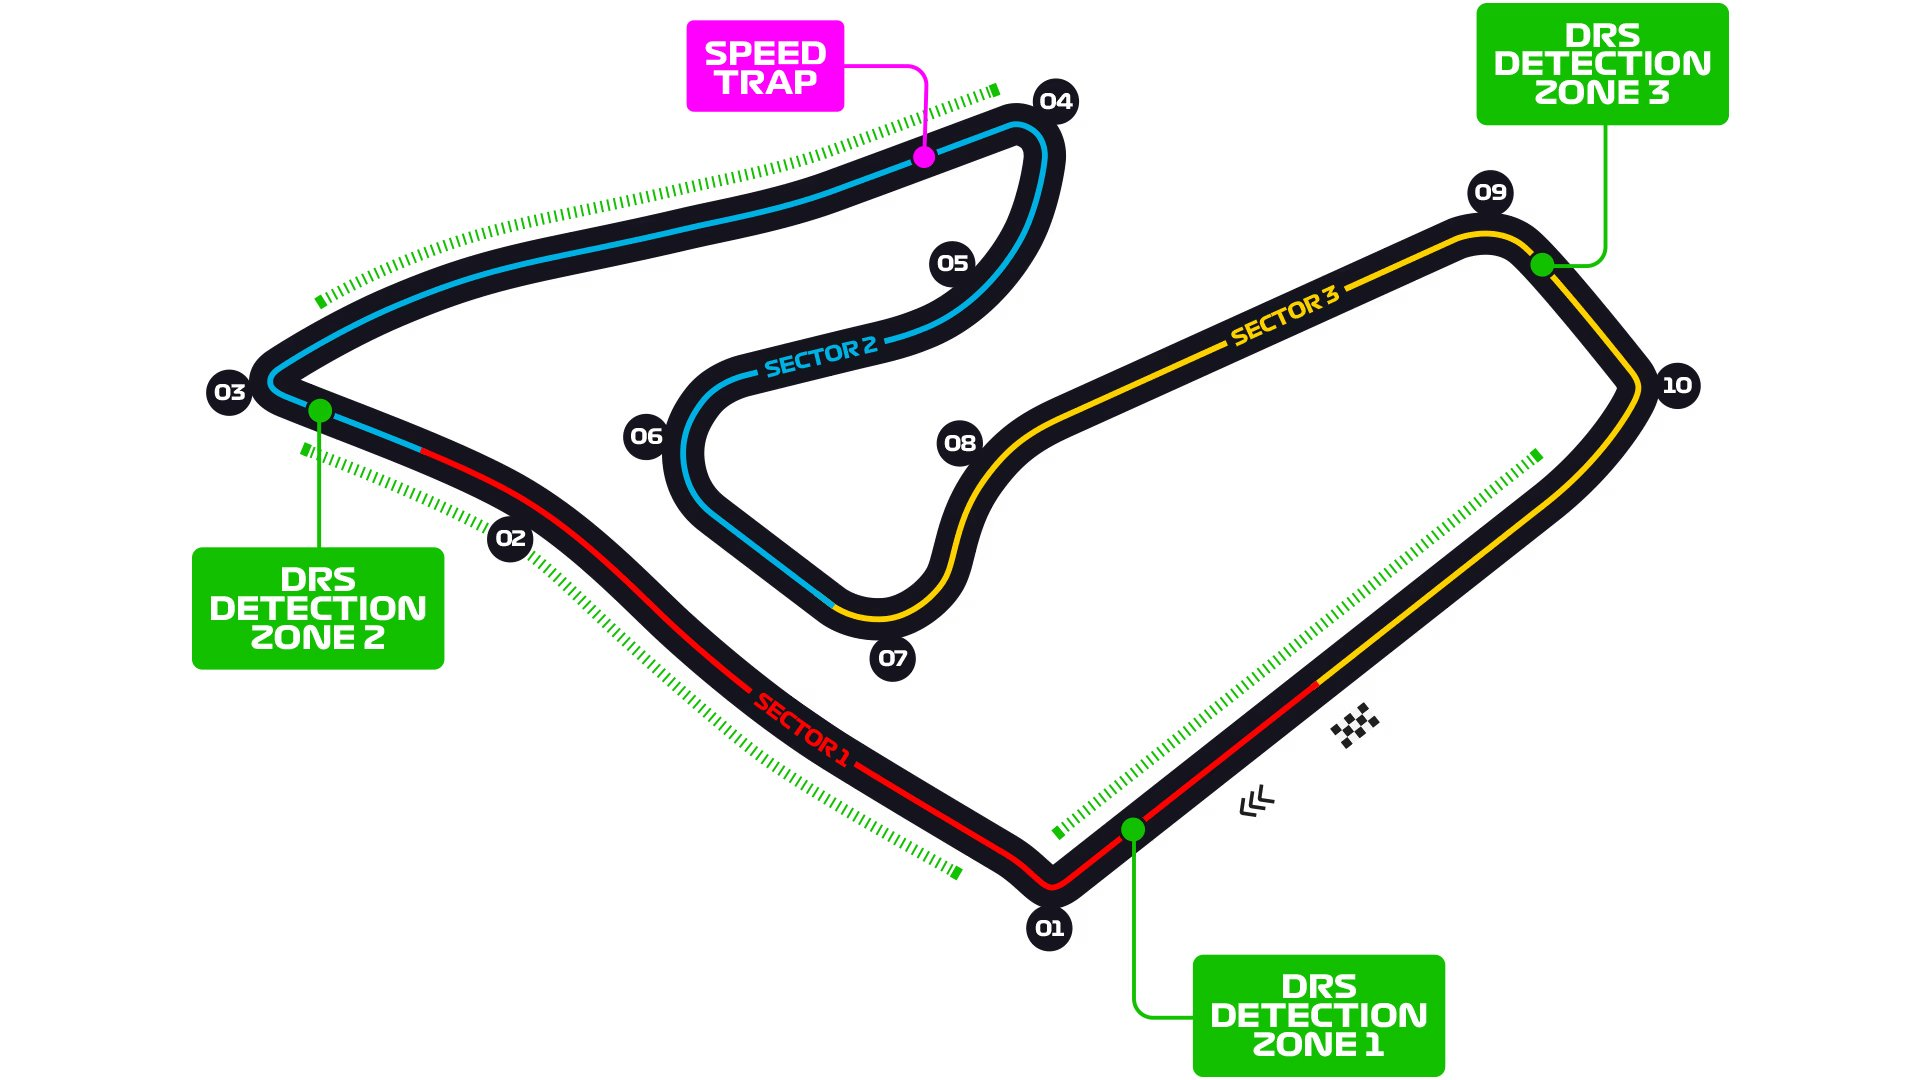
\includegraphics[width=0.75\linewidth]{images/11.Austria_Circuit.jpg}
\end{figure}

\begin{itemize}
    \item \textbf{Lap Record} : 1:02.939 (2020, Valtteri Bottas – Mercedes).
    
    \item \textbf{Number of Corners \& Key Features} : 10 turns (7 right, 3 left) - Short, fast lap with big elevation changes. Mix of long straights and heavy braking zones.
    
    \item \textbf{Braking Zones \& Traction} : Three heavy braking zones at Turns 1, 3, and 4. Strong traction out of slow corners critical to lap time and overtaking.

    \item \textbf{DRS \& Overtaking} : Three DRS zones (main straight, before Turn 3, before Turn 4). \\
    Overtaking opportunities primarily at Turns 3 and 4.
    
    \item \textbf{Tyre Degradation \& Strategy} : Track is usually low degradation but traction zones stress rear tyres.\\
    Two-stop strategies common, but one-stop sometimes possible with tyre management.
    
    \item \textbf{Weather \& Environment} : Mountain climate can bring sudden rain.\\
    High altitude reduces downforce and engine power, favouring efficient aero packages.
\end{itemize}

\textbf{Strategic Summary :}
The Red Bull Ring rewards cars with straight-line speed, strong braking, and traction. Short lap amplifies traffic management in qualifying and strategy timing during the race.


\subsection{Race Analysis}

\textbf{Date:} Sprint : 29 June 2024 - 12:00 local time\\
Race : 30 June 2024 — 15:00 local time 

\begin{itemize}
    \item \textbf{Sprint Qualifying:} \textbf{Pole Position:} Max Verstappen (Red Bull) – 1:04.686.\\
    Grid : Norris 2nd, Piastri 3rd, Russell 4th.

    \item \textbf{Sprint Summary} : \textbf{Winner:} Max Verstappen (Red Bull). \\
    \textbf{Podium}: 1. Verstappen - 2. Piastri - 3. Norris. \\
    Norris briefly overtook Verstappen into Turn 3 but was repassed; Piastri also attacked but couldn’t convert.
    
    \item \textbf{Qualifying Summary} : \textbf{Pole Position:} Max Verstappen (Red Bull) – 1:04.314. \\
    Grid: Norris 2nd, Russell 3rd, Sainz 4th.
    
    \item \textbf{Race Summary} : \textbf{Winner:} George Russell (Mercedes).\\
    \textbf{Podium:} 1. Russell - 2. Piastri - 3. Sainz.\\
    \textbf{Notable incidents:} Verstappen–Norris collision at Turn 3, 6 laps before the end (Virtual Safety Car deployed late after).
    
    \item \textbf{Strategies} : Most teams on two-stop strategies (Medium–Hard–Medium).\\
    - Verstappen and Norris ran aggressive stints, pushing hard early, leading to tyre wear and tension in final laps. \\
    - Russell and Mercedes opted for a conservative but well-executed Medium–Hard–Hard, staying in contention. \\
    - Piastri extended his middle stint, allowing fresher tyres to overtake Sainz late for P2. \\
    - Ferrari mirrored McLaren but couldn’t match pace. Leclerc lost out with traffic and track limits, finishing P11.\\
    - Haas split strategies: both Hülkenberg and Magnussen scored strong points with consistent tyre management.
    
    \item \textbf{Performance Trends} : \textbf{Mercedes:} Opportunistic and precise. Russell’s consistency brought first win since Brazil 2022. Hamilton solid P4 despite a 5s penalty. \\
    \textbf{McLaren:} Fastest car overall, but Norris’s clash wasted a possible win. Piastri salvaged superb P2. \\
    \textbf{Red Bull:} Verstappen dominant until collision, Pérez mediocre (P7). First cracks in home dominance. \\
    \textbf{Ferrari:} Sainz consistent P3; Leclerc struggled with pace and penalties, finishing out of points. \\
    \textbf{Haas:} Standout of midfield — double points (Hülkenberg P6, Magnussen P8).
    
    \item \textbf{Championship Impact} : \textbf{Drivers:} Verstappen 237 points, Norris 156, Leclerc 150.\\
    \textbf{Constructors:} Red Bull 355, Ferrari 291, McLaren 268, Mercedes 196.    
\end{itemize}

\textbf{Key Takeaway :}
The Verstappen–Norris clash opened the door for Russell and Mercedes. McLaren again showed genuine race-winning speed, while Ferrari continued consistent podium scoring. Red Bull’s dominance cracked under pressure at their home race.


\subsection{Link \& Takeaway}

\begin{itemize}
    \item The Red Bull Ring’s heavy braking zones and traction battles suited Red Bull and McLaren, explaining their duel at the front. 
    \item Mercedes capitalised perfectly when fortune turned, confirming progress. 
    \item Ferrari again lacked the ultimate pace but benefited from rivals’ misfortune.
    \item Haas delivered their best weekend in years, while Aston Martin continued to decline.
\end{itemize}
\section{British Grand prix}

\subsection{Circuit Analysis}

\textbf{Circuit Name:} Silverstone Circuit (Silverstone, United Kingdom) \\
\textbf{Length:} 5.891 km - \textbf{Laps:} 52 - \textbf{Total Distance:} 306.198 km

\begin{figure}[H]
    \centering
    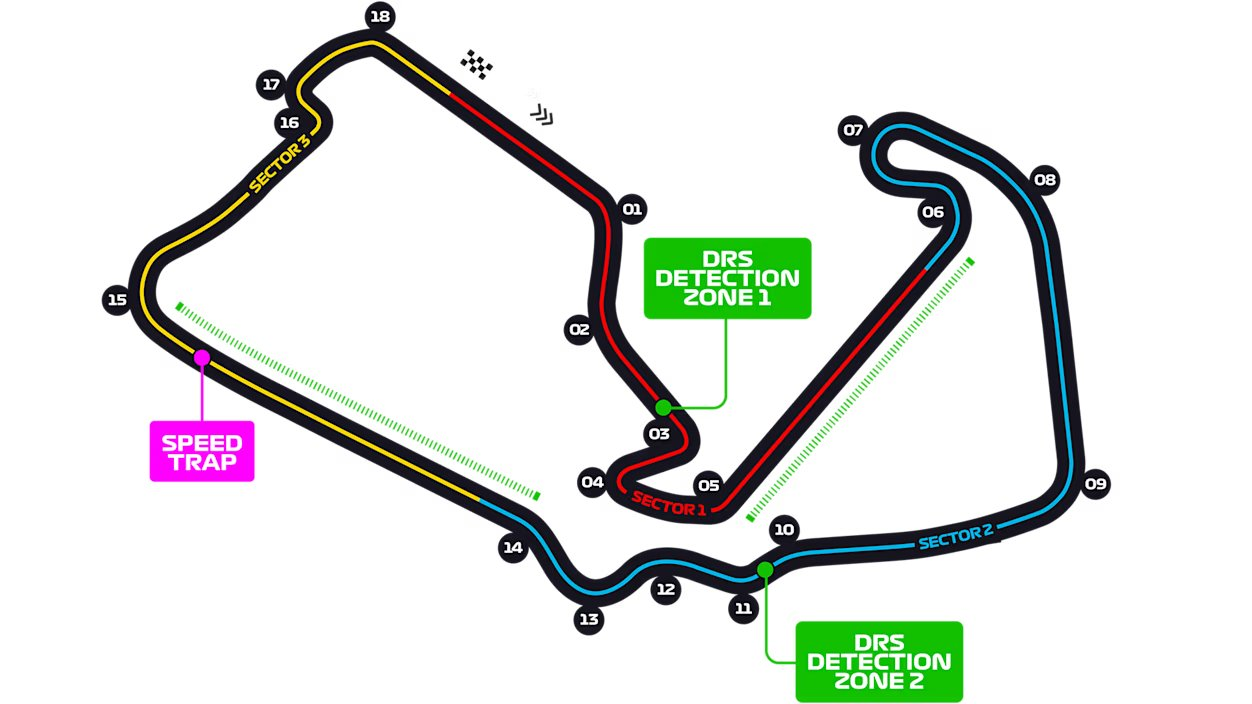
\includegraphics[width=0.75\linewidth]{images/12.Great_Britain_Circuit.jpg}
\end{figure}


\begin{itemize}
    \item \textbf{Lap Record} : 1:25.093 (2017, Lewis Hamilton – Mercedes).
    
    \item \textbf{Number of Corners \& Key Features} : 18 turns (10 right, 8 left) - High-speed classic featuring iconic sections: Maggots–Becketts–Chapel, Copse, Stowe. \\
    Combination of fast corners and technical complexes makes Silverstone a complete car test.
    
    \item \textbf{Braking Zones \& Traction} : Not many heavy braking zones, main ones at Turn 3 (Village) and Turn 16 (Vale).\\
    Traction important out of Club corner onto main straight.

    \item \textbf{DRS \& Overtaking} : Two DRS zones (Wellington straight, Hangar straight).\\
    Main overtaking at Brooklands (Turn 6) and Stowe (Turn 15).
    
    \item \textbf{Tyre Degradation \& Strategy} : High-energy corners stress tyres, especially fronts. Two-stop strategies typical.\\
    Tyre management crucial in long stints.
    
    \item \textbf{Weather \& Environment} : British summer weather often unpredictable: wind, rain possible. Cooler temperatures affect tyre warm-up.
\end{itemize}

\textbf{Strategic Summary :}
Silverstone demands aerodynamic efficiency, high-speed stability, and strong tyre management. 
It is one of the ultimate tests of chassis balance and aerodynamic performance.


\subsection{Race Analysis}

\textbf{Date:} 7 July 2024 — 15:00 local time 

\begin{itemize}
    \item \textbf{Qualifying Summary} : \textbf{Pole Position:} George Russell (Mercedes) – 1:25.819. \\
    Grid: Hamilton 2nd, Norris 3rd, Verstappen 4th.
    
    \item \textbf{Race Summary} : \textbf{Winner:} Lewis Hamilton (Mercedes) - his 104th career victory, first since 2021.\\
    \textbf{Podium:} 1. Hamilton - 2. Verstappen - 3. Norris.\\
    \textbf{Technical issues:} Russell (hydraulic problem).
    
    \item \textbf{Strategies} : 
    - Mercedes: Hamilton on Medium–Inter–Soft, perfectly timed pit windows during rain/slick crossover. \\
    - Red Bull: Verstappen ran Medium–Inter–Hard, lacking late grip vs Hamilton’s softs. \\
    - McLaren: Norris and Piastri delayed stops in changing weather — lost track position. \\
    - Ferrari: Sainz salvaged P5 + fastest lap, Leclerc stuck in midfield with wrong calls. \\
    - Haas: Hülkenberg brilliant P6, maximizing consistency in mixed conditions. \\
    - Aston Martin: Both cars in points (Stroll P7, Alonso P8). \\
    - Williams \& Racing Bulls: Albon P9, Tsunoda P10, opportunistic in changing conditions.
    
    \item \textbf{Performance Trends} : 
    \textbf{Mercedes} delivered their best weekend: Hamilton mastered tyre changes and pressure, Russell unlucky. \\
    \textbf{Red Bull} lacked dominance, Verstappen still consistent with P2. \\
    \textbf{McLaren} had winning pace but strategy errors cost Norris a shot at victory. \\
    \textbf{Ferrari} disappointed, strategy again the weak point. \\
    \textbf{Haas} strong midfield pace, outperforming Aston Martin at times. \\
    \textbf{Williams \& Racing Bulls} scored valuable points, Alpine absent from the fight.
    
    \item \textbf{Championship Impact} : \textbf{Drivers:} Verstappen 255 points, Norris 171, Leclerc 150.\\
    \textbf{Constructors:} Red Bull 373, Ferrari 302, McLaren 295, Mercedes 221.    
\end{itemize}

\textbf{Key Takeaway :}
Hamilton’s masterful tyre management and strategy earned him an emotional home win. Red Bull maintained points lead, McLaren kept momentum, Ferrari slipped back.


\subsection{Link \& Takeaway}

\begin{itemize}
    \item Silverstone’s high-speed corners rewarded Mercedes’ improved aero package, allowing Hamilton to win.
    \item Verstappen and Red Bull remained consistent, but strategy limited their challenge for victory.
    \item McLaren showed podium pace but lacked decisive execution to fight for P1.
    \item Ferrari’s lack of adaptability exposed their weaknesses on high-energy tracks.
    \item Midfield fight remains tight: Haas, Aston Martin, and Williams all capitalized on chaos. 
\end{itemize}
\section{Hungarian Grand prix}

\subsection{Circuit Analysis}

\textbf{Circuit Name:} Hungaroring (Mogyoród, Hungary) \\
\textbf{Length:} 4.381 km - \textbf{Laps:} 70 - \textbf{Total Distance:} 306.630 km

\begin{figure}[H]
    \centering
    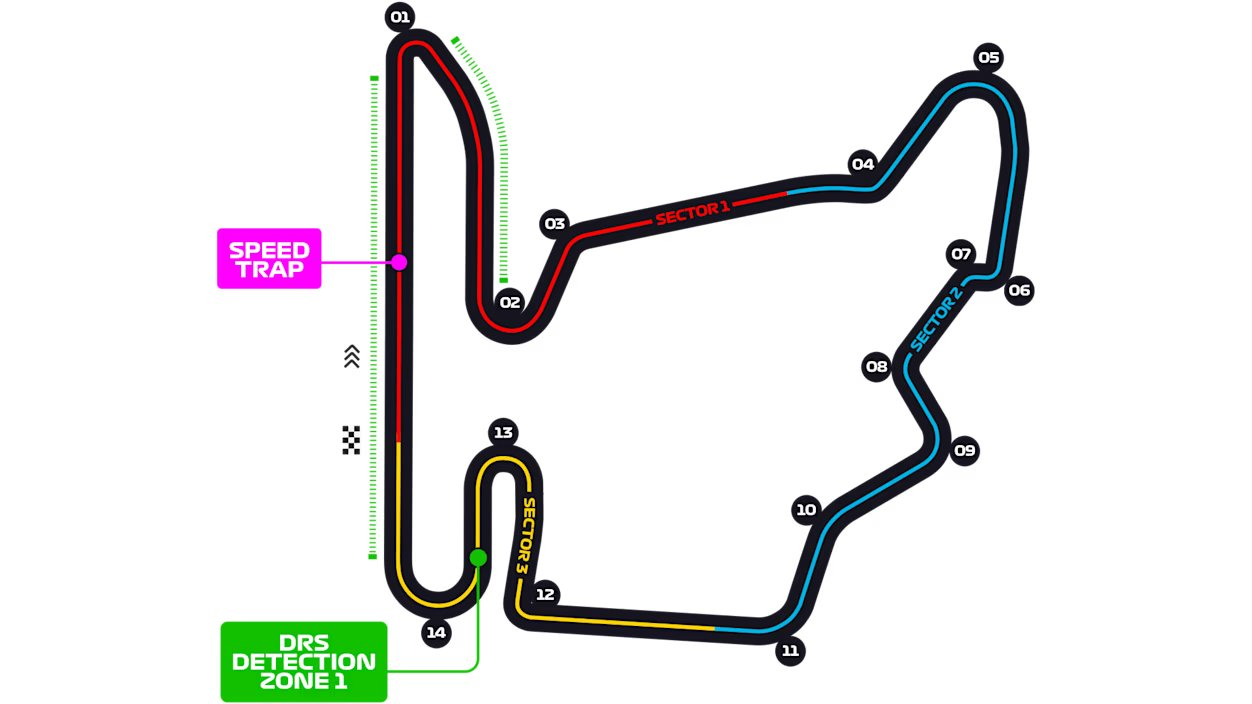
\includegraphics[width=0.75\linewidth]{images/13.Hungary_Circuit.jpg}
\end{figure}


\begin{itemize}
    \item \textbf{Lap Record} : 1:13.447 (2020, Lewis Hamilton – Mercedes).
    
    \item \textbf{Number of Corners \& Key Features} : 14 turns (8 right, 6 left). \\
    Tight and twisty layout, often compared to a "Monaco without walls". High downforce required, limited straights.
    
    \item \textbf{Braking Zones \& Traction} : Heavy braking into Turn 1 (prime overtaking spot) and Turn 12. \\
    Good traction needed out of slow corners to maximise lap time.

    \item \textbf{DRS \& Overtaking} : Two DRS zones (main straight, between Turns 1–2). \\
    Overtaking is difficult due to narrow track and dirty air effect.
    
    \item \textbf{Tyre Degradation \& Strategy} : Circuit demands high downforce and consistent tyre management. \\
    Two-stop strategies typical due to heat and high corner load. 
    
    \item \textbf{Weather \& Environment} : Hot Hungarian summers push tyre temperatures to extremes. \\
    Dusty track surface early in the weekend increases evolution.
\end{itemize}

\textbf{Strategic Summary :}
Hungaroring rewards cars with strong downforce and drivers with precision. Track position is crucial, as overtaking is rare. Heat and tyre wear often decide strategy, making two-stoppers the norm.


\subsection{Race Analysis}

\textbf{Date:} 21 July 2024 — 15:00 local time 

\begin{itemize}
    \item \textbf{Qualifying Summary} : \textbf{Pole Position:} Lando Norris (McLaren) – 1:15.227. \\
    Grid: Piastri 2nd, Verstappen 3rd, Sainz 4th.
    
    \item \textbf{Race Summary} : \textbf{Winner:} Oscar Piastri (McLaren) - his first F1 victory.\\
    \textbf{Podium:} 1. Piastri - 2. Norris - 3. Hamilton.\\
    \textbf{Technical issues:} Gasly (hydraulic problem).\\
    Piastri jumped Norris at start, controlled pace. Hamilton undercut to beat Ferrari. Verstappen struggled with balance, finishing only P5.
    
    \item \textbf{Strategies} : Most front-runners on two-stop strategies (Medium–Hard–Medium). \\
    - McLaren: Piastri gained track position at Turn 1 start, stayed ahead all race. Norris lost time at slow pit stop, finishing P2. \\ 
    - Mercedes: Hamilton on Medium–Hard–Medium. Extended middle stint to overcut Ferrari, securing podium. Russell (17th → 8th + fastest lap) maximised recovery with aggressive undercuts. \\
    - Ferrari: Leclerc on Medium–Hard–Medium, steady pace for P4. Sainz ran Medium–Medium–Hard but lost time late due to tyre wear, P6. \\
    - Red Bull: Verstappen struggled with rear grip, ran Medium–Hard–Hard, unable to challenge podium, P5. Pérez recovered from P16 to P7 on offset Medium–Hard–Medium.
    
    \item \textbf{Performance Trends} : \textbf{McLaren} dominant — car suited Hungaroring perfectly. \\
    Mercedes competitive in race pace. \\
    Ferrari stable but lacking podium pace. \\
    Red Bull off-form — Verstappen complained of poor traction and balance. \\
    Aston Martin and Racing Bulls scrapping for lower points, Haas faded.
    
    \item \textbf{Championship Impact} : \textbf{Drivers:} Verstappen 265 points, Norris 189, Leclerc 162.\\
    \textbf{Constructors:} Red Bull 389, McLaren 338 (+1), Ferrari 322 (-1), Mercedes 241.    
\end{itemize}

\textbf{Key Takeaway :}
McLaren dominated Hungary, with Piastri claiming his first F1 win and Norris close behind. Mercedes showed strong pace, while Red Bull and Ferrari lagged, shifting the competitive balance in the title race.


\subsection{Link \& Takeaway}

\begin{itemize}
    \item Hungaroring’s high-downforce, twisty layout exposed Red Bull’s weaknesses and amplified McLaren’s strengths. 
    \item Piastri’s flawless race execution secured a breakthrough victory, marking him as a genuine contender. 
    \item Norris reinforced McLaren’s strength but lost out via pit stop delay. 
    \item Hamilton’s podium underlined Mercedes’ progress, Russell’s comeback + fastest lap highlighted pace recovery. 
    \item Ferrari maintained consistency but couldn’t match McLaren/Mercedes. 
    \item Aston Martin, Haas, Alpine, and Williams again struggled for points in a tight midfield.
\end{itemize}
\section{Belgian Grand prix}

\subsection{Circuit Analysis}

\textbf{Circuit Name:} Circuit de Spa-Francorchamps (Stavelot, Belgium) \\
\textbf{Length:} 7.004 km - \textbf{Laps:} 44 - \textbf{Total Distance:} 308.052 km

\begin{figure}[H]
    \centering
    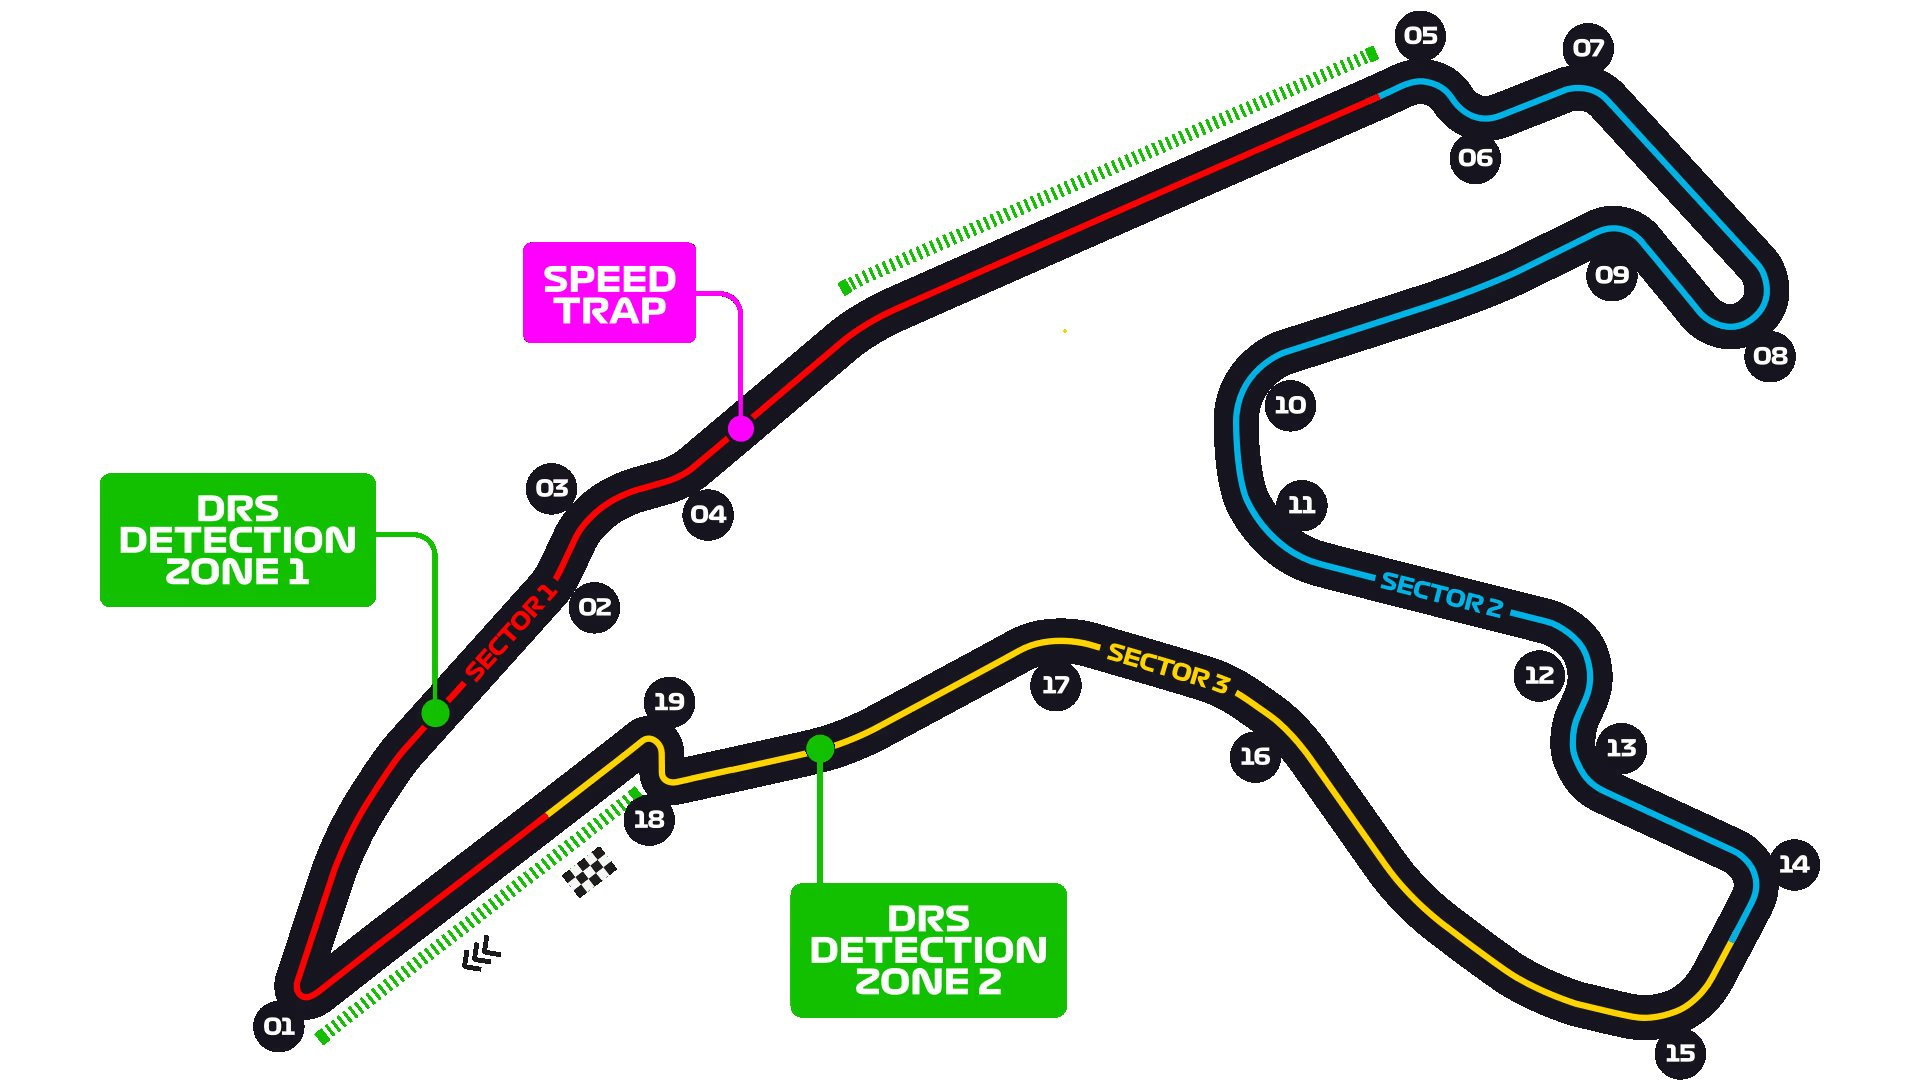
\includegraphics[width=0.75\linewidth]{images/14.Belgium_Circuit.jpg}
\end{figure}


\begin{itemize}
    \item \textbf{Lap Record} : 1:41.252 (2020, Lewis Hamilton – Mercedes).
    
    \item \textbf{Number of Corners \& Key Features} : 19 turns (10 right, 9 left). \\
    Iconic corners include Eau Rouge–Raidillon, Pouhon, and Blanchimont. High-speed circuit with major elevation changes.
    
    \item \textbf{Braking Zones \& Traction} : Heavy braking at La Source (Turn 1), Les Combes (Turn 5), and the Bus Stop chicane (Turns 18–19). \\
    Traction critical at exits of La Source and Turn 1 leading to long acceleration phases.
    
    \item \textbf{DRS \& Overtaking} : Two DRS zones (Kemmel straight, start/finish straight). \\
    Overtaking opportunities primarily at Les Combes and the Bus Stop chicane.
    
    \item \textbf{Tyre Degradation \& Strategy} : Medium degradation, with high lateral loads stressing tyres through fast corners. \\
    Two-stop strategies typical, but a one-stop can be attempted if conditions allow.
    
    \item \textbf{Weather \& Environment} : Famous for unpredictable Ardennes weather. \\
    Sudden showers possible, creating mixed conditions across different sectors of the track.
\end{itemize}

\textbf{Strategic Summary :} Spa demands aerodynamic efficiency, straight-line speed, and tyre management. Overtaking is more feasible than most tracks, but weather and Safety Cars often dictate race outcomes.

\subsection{Race Analysis}
\textbf{Date:} 28 July 2024 — 15:00 local time

\begin{itemize}
    \item \textbf{Qualifying Summary} : \textbf{Pole Position:} Charles Leclerc – 1:53.754. \\
    \textbf{Fastest lap in Q3:} Max Verstappen (Red Bull) – 1:53.159. \\
    Grid: Leclerc 1st, Pérez 2nd, Hamilton 3rd, Norris 4th.\\
    Max Verstappen, who finished 1st during the qualifications, was penalised of ten grid places for changing propulsion system components outside the quota.
    
    \item \textbf{Race Summary} : \textbf{Winner:} Lewis Hamilton (Mercedes) — back-to-back win after Hungary podium. \\
    \textbf{Podium:} 1. Hamilton - 2. Piastri - 3. Leclerc. \\
    Verstappen recovered from P11 to P4. \\
    Russell initially P1 but later disqualified for car underweight.\\
    
    \item \textbf{Strategies} : A race of fine margins under variable Spa weather. \\
    - Mercedes: Hamilton executed Medium–Hard–Medium, managing tyre wear superbly. Russell ran aggressive Medium–Medium–Hard, leading laps before DSQ. \\
    - McLaren: Piastri mirrored Hamilton’s Medium–Hard–Medium and almost stole victory on fresher tyres in final laps. Norris ran Medium–Hard–Medium as well, finishing P5. \\
    - Ferrari: Leclerc P3 (Medium–Hard–Medium), steady but lacked pace to fight Hamilton/Piastri. Sainz P6 with Medium–Hard–Hard. \\
    - Red Bull: Verstappen Medium–Hard–Hard, fast recovery drive but hindered by traffic. Pérez started P2, faded with tyre wear (P7) but took fastest lap. \\
    - Aston Martin: Alonso P8 and Stroll P11, both on Medium–Hard. \\
    - Alpine: Ocon P9, Gasly P13, solid midfield points. \\
    - Racing Bulls: Ricciardo P10, Tsunoda P16 — consistent but off the pace.
    
    \item \textbf{Performance Trends} : \textbf{Mercedes} showed their strongest pace of 2024, Hamilton mastering Spa’s conditions. \\
    \textbf{McLaren} were highly competitive, Piastri nearly winning. \\
    \textbf{Ferrari} consistent but again short of outright victory. \\
    \textbf{Red Bull} compromised by grid penalties and weak race execution — Verstappen only P4, Pérez P7. \\
    \textbf{Midfield}: Alpine and Aston Martin snatched points, Haas and Kick Sauber anonymous.
    
    \item \textbf{Championship Impact} : \textbf{Drivers:} Verstappen 277, Norris 199, Leclerc 177. \\
    \textbf{Constructors:} Red Bull 408, McLaren 366, Ferrari 345, Mercedes 266.
\end{itemize}

\textbf{Key Takeaway :} Hamilton triumphed at Spa thanks to perfect tyre management and strategy, resisting a late charge from Piastri. Ferrari showed consistency, while Red Bull’s struggles from poor grid positions limited their damage control.


\subsection{Link \& Takeaway}

\begin{itemize}
    \item Spa’s long straights and mixed-weather traits rewarded Mercedes’ strong balance and Hamilton’s experience. 
    \item McLaren’s race pace was excellent, with Piastri nearly stealing the win in the final laps. 
    \item Ferrari matched expectations with stable tyre life but lacked ultimate pace to challenge for victory. 
    \item Red Bull’s vulnerability from grid penalties showed how track position and execution are crucial at Spa. 
\end{itemize}
\section{Dutch Grand Prix}

\subsection{Circuit Analysis}

\textbf{Circuit Name:} Circuit Zandvoort (Zandvoort, Netherlands) \\
\textbf{Length:} 4.259 km - \textbf{Laps:} 72 - \textbf{Total Distance:} 306.587 km

\begin{figure}[H]
    \centering
    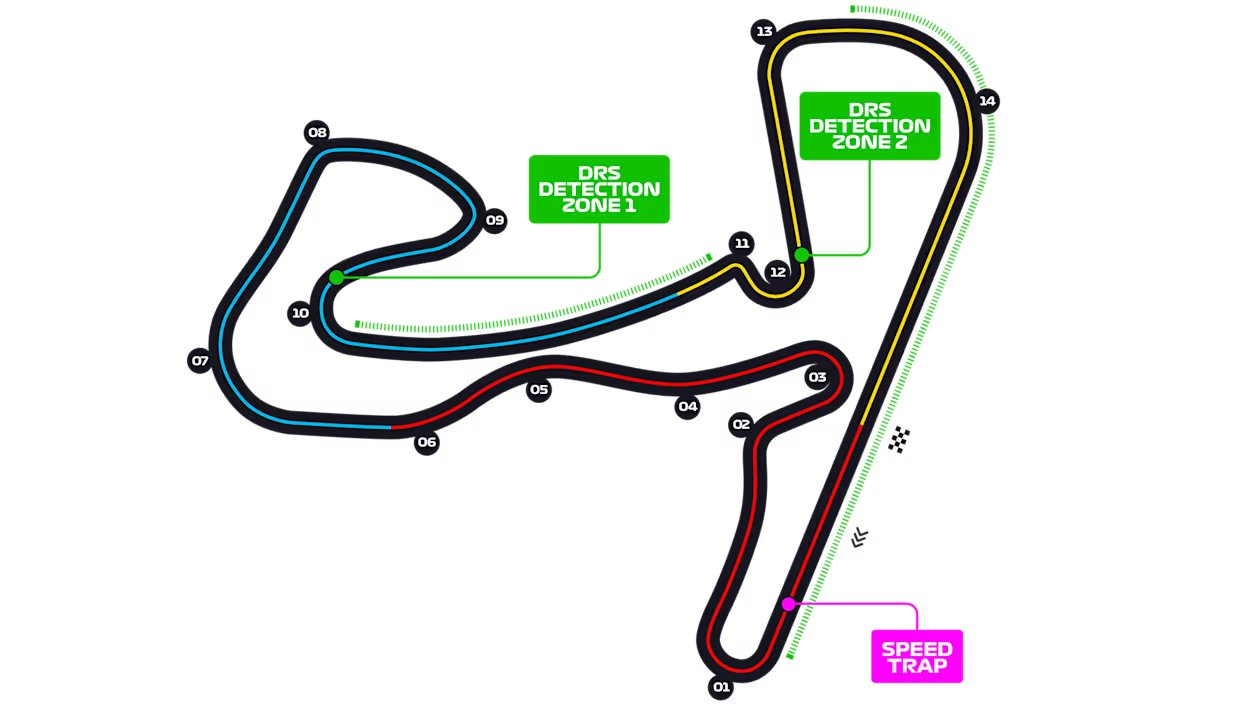
\includegraphics[width=0.75\linewidth]{images/15.Netherlands_Circuit.jpg}
\end{figure}

\begin{itemize}
    \item \textbf{Lap Record} : 1:08.885 (2021, Max Verstappen – Red Bull).
    
    \item \textbf{Number of Corners \& Key Features} : 14 turns (10 right, 4 left). \\
    Famous for banked corners (notably Turn 3 “Hugenholtzbocht” and Turn 14 “Arie Luyendykbocht”). \\
    Narrow track with limited overtaking zones, high emphasis on qualifying.
    
    \item \textbf{Braking Zones \& Traction} : Heavy braking into Turn 1 (Tarzanbocht) is the prime overtaking spot. \\
    Strong traction needed out of the banked final corner to maximize speed on the main straight.
    
    \item \textbf{DRS \& Overtaking} : Two DRS zones (main straight, between Turns 10 and 11). \\
    Overtaking difficult outside of Turn 1 due to narrow layout.
    
    \item \textbf{Tyre Degradation \& Strategy} : High-load corners stress tyres. \\
    Two-stop strategies standard, with high wear on soft compound.
    
    \item \textbf{Weather \& Environment} : Coastal winds and sand from the dunes reduce grip. \\
    Track evolution is significant, demanding constant adaptation.
\end{itemize}

\textbf{Strategic Summary :} Zandvoort rewards qualifying performance, tyre management, and aerodynamic efficiency. The narrow layout limits overtaking, making pit strategy and track position crucial.

\subsection{Race Analysis}

\textbf{Date:} 25 August 2024 — 15:00 local time 

\begin{itemize}
    \item \textbf{Qualifying Summary} : \textbf{Pole Position:} Lando Norris (McLaren) – 1:09.673. \\
    Grid: Verstappen 2nd, Piastri 3rd, Russell 4th. \\
    Hamilton only 14th due to a three grid places penalty, Albon disqualified from qualifying.
    
    \item \textbf{Race Summary} : \textbf{Winner:} Lando Norris (McLaren) — his first hat-trick (pole, win, fastest lap). \\
    \textbf{Podium:} 1. Norris - 2. Verstappen - 3. Leclerc. \\
    No retirements, marking a record fourth GP of the season without DNFs.
    
    \item \textbf{Strategies} : Two-stop race standard across the grid. \\
    - Verstappen led laps 1–17 but lost out on tyre wear. \\
    - Norris retook the lead mid-race and secured victory with fastest lap on the final tour. \\
    - Piastri briefly led (laps 29–32) before dropping behind due to tyre degradation.
    
    \item \textbf{Performance Trends} : 
    \textbf{McLaren:} Norris dominant, Piastri competitive throughout. Clear tyre advantage in long runs. \\
    \textbf{Red Bull:} Verstappen fought hard at home but tyre wear limited his late pace, Pérez underwhelming P6. \\
    \textbf{Ferrari:} Leclerc solid podium, Sainz strong recovery drive to P5. \\
    \textbf{Mercedes:} Russell P7, Hamilton P8 from P14, lacked outright pace compared to rivals. \\
    \textbf{Alpine \& Aston Martin:} Gasly scored again (P9), Alonso took last point (P10).
    
    \item \textbf{Championship Impact} : \textbf{Drivers:} Verstappen 295 pts, Norris 225, Leclerc 192. \\
    \textbf{Constructors:} Red Bull 434, McLaren 404, Ferrari 370, Mercedes 276.
\end{itemize}

\textbf{Key Takeaway :} Lando Norris delivered a flawless weekend, securing pole, victory, and fastest lap for McLaren’s resurgence. Ferrari remained consistent, while Mercedes struggled to extract performance.

\subsection{Link \& Takeaway}

\begin{itemize}
    \item Zandvoort’s narrow layout and banked corners heavily favored track position, McLaren maximized this with Norris’ pole and perfect execution. 
    \item Verstappen’s home GP showed Red Bull’s vulnerability on tyre wear compared to McLaren. 
    \item Ferrari confirmed itself as the “constant podium” team, while Mercedes’ pace deficit became evident. 
    \item The race highlighted McLaren’s transformation into a true championship challenger.
\end{itemize}

\section{Italian Grand Prix}

\subsection{Circuit Analysis}

\textbf{Circuit Name:} Autodromo Nazionale di Monza (Monza, Italy) \\
\textbf{Length:} 5.793 km - \textbf{Laps:} 53 - \textbf{Total Distance:} 306.720 km

\begin{figure}[H]
    \centering
    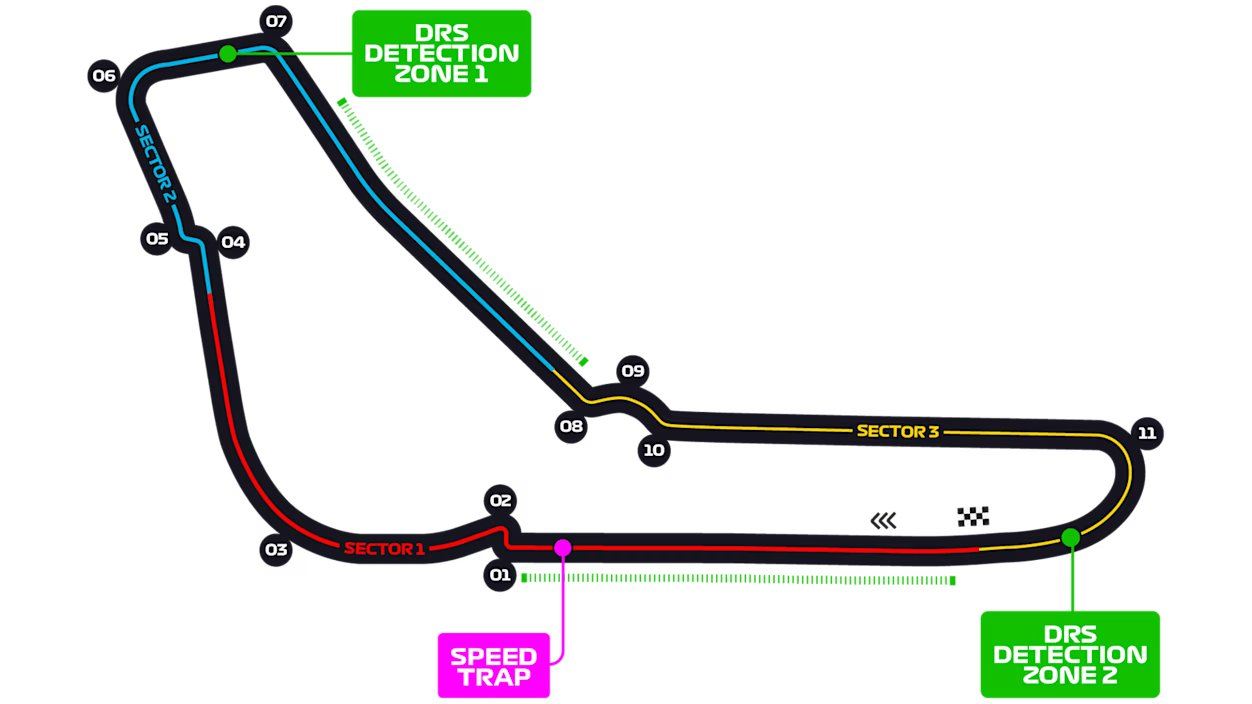
\includegraphics[width=0.75\linewidth]{images/16.Italy_Circuit.jpg}
\end{figure}

\begin{itemize}
    \item \textbf{Lap Record} : 1:18.887 (2020, Lewis Hamilton – Mercedes).
    
    \item \textbf{Number of Corners \& Key Features} : 11 turns (7 right, 4 left). \\
    Known as the “Temple of Speed”: long straights, chicanes (Rettifilo, Roggia), fast Lesmo corners, Ascari chicane, and the iconic Parabolica. \\
    Cars run minimum downforce to maximise top speed.
    
    \item \textbf{Braking Zones \& Traction} : Heavy braking zones at Turn 1 (Rettifilo) and Turn 4 (Roggia). \\
    Traction crucial out of Parabolica to carry speed onto main straight.
    
    \item \textbf{DRS \& Overtaking} : Two DRS zones (main straight, between Lesmo 2 and Ascari). \\
    Main overtaking into Rettifilo chicane, Ascari also provides opportunities.
    
    \item \textbf{Tyre Degradation \& Strategy} : Low tyre wear overall, but traction zones stress rears. \\
    One-stop possible but risky, two-stop often preferred.
    
    \item \textbf{Weather \& Environment} : Warm, stable late-summer weather. \\
    Huge tifosi support makes Monza Ferrari’s home fortress.
\end{itemize}

\textbf{Strategic Summary :} Monza rewards straight-line efficiency, braking stability, and clean pit execution. Track position is critical given DRS trains and limited overtaking beyond Turn 1.


\subsection{Race Analysis}

\textbf{Date:} 1 September 2024 — 15:00 local time 

\begin{itemize}
    \item \textbf{Qualifying Summary} : \textbf{Pole Position:} Lando Norris (McLaren) – 1:19.327. \\
    Grid: Piastri 2nd, Russell 3rd, Leclerc 4th.\\
    Franco Colapinto debuted with Williams, replacing Sargeant.
    
    \item \textbf{Race Summary} : \textbf{Winner: Charles Leclerc (Ferrari)}. \\
    \textbf{Podium:} 1. Leclerc - 2. Piastri - 3. Norris. \\
    Verstappen salvaged P6 in a difficult weekend for Red Bull.
    
    \item \textbf{Strategies} : 
    - Ferrari: Leclerc bold one-stop (Medium–Hard, 38 laps on hards). Perfect tyre management secured win. \\
    - McLaren: Piastri led early, forced to pit twice, Norris attempted undercut on Leclerc but lost track position. Both lacked tyre longevity. \\
    - Mercedes: Hamilton and Russell solid but lacked pace to fight podium. \\
    - Red Bull: Verstappen struggled on degradation, Pérez P8. \\
    - Midfield: Albon P9 strong for Williams. Haas in points despite penalties.
    
    \item \textbf{Performance Trends} :  
    \textbf{Ferrari:} Brilliant strategy and execution, Leclerc calm under pressure. Sainz strong support in P4. \\
    \textbf{McLaren:} Fastest in raw pace but outsmarted strategically. \\
    \textbf{Mercedes:} Consistent, but podium pace lacking. \\
    \textbf{Red Bull:} Fourth-best team — Verstappen frustrated, Pérez mediocre. \\
    \textbf{Midfield:} Williams (Albon) reliable, Haas scrappy points, Aston Martin invisible.
    
    \item \textbf{Championship Impact} : \textbf{Drivers:} Verstappen 303 pts, Norris 241, Leclerc 217. \\
    \textbf{Constructors:} Red Bull 446, McLaren 438, Ferrari 407, Mercedes 292
\end{itemize}

\textbf{Key Takeaway :} Charles Leclerc delivered an emotional victory at Monza with a masterful one-stop strategy, delighting the tifosi. McLaren proved the fastest team but paid for higher tyre wear. Red Bull faltered again, leaving Verstappen under pressure as the title fight tightened dramatically.

\subsection{Link \& Takeaway}

\begin{itemize}
    \item Ferrari’s home win emphasized strategic brilliance and Leclerc’s calm under pressure. 
    \item McLaren lost a win despite dominance in qualifying — tyre management still a weakness. 
    \item Red Bull continued to struggle, raising concerns about their position as championship leaders. 
    \item Mercedes remained consistent but lacked podium pace.
    \item The championship battle tightened further: Verstappen still leads but Norris, Leclerc, and Piastri are closing in.
\end{itemize}

\section{Azerbaijan Grand Prix}

\subsection{Circuit Analysis}

\textbf{Circuit Name:} Baku City Circuit (Baku, Azerbaijan) \\
\textbf{Length:} 6.003 km - \textbf{Laps:} 51 - \textbf{Total Distance:} 306.049 km

\begin{figure}[H]
    \centering
    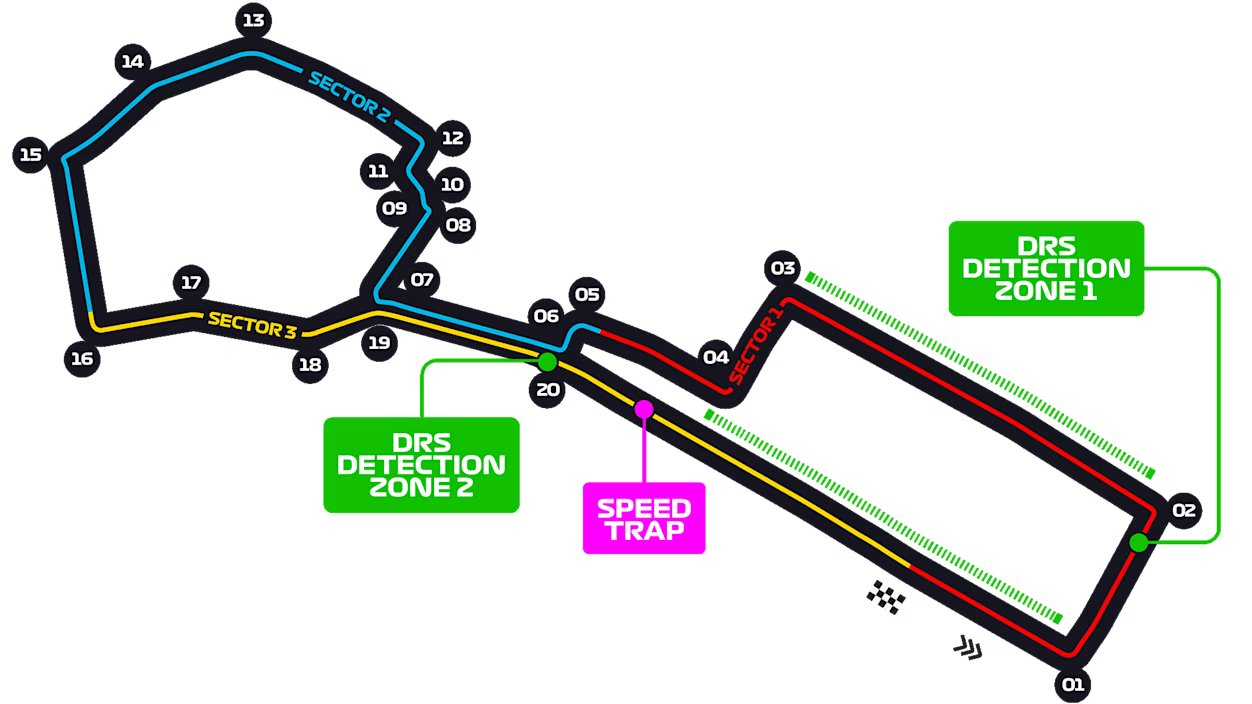
\includegraphics[width=0.75\linewidth]{images/17.Azerbaijan_Circuit.jpg}
\end{figure}

\begin{itemize}
    \item \textbf{Lap Record} : 1:40.203 (2023, Charles Leclerc – Ferrari).

    \item \textbf{Number of Corners \& Key Features} : 20 turns (8 right, 12 left). \\
    Longest straight (2.2 km) with DRS, mixed with narrow old town section (Turns 8–12). \\
    Demands low downforce for speed yet stability for traction/braking in tight corners.

    \item \textbf{Braking Zones \& Traction} : Major braking at Turn 1 (end of main straight), Turn 3, and Turn 15. \\
    Rear traction out of low-speed corners is critical, especially final corner before the main straight.

    \item \textbf{DRS \& Overtaking} : Two main DRS zones (main straight and between Turns 2–3). \\
    Prime overtaking into Turn 1, opportunistic moves possible at Turn 3.

    \item \textbf{Tyre Degradation \& Strategy} : Surface relatively smooth → low wear, but rear degradation can spike due to traction zones. \\
    Safety Car probability is high, influencing flexible tyre strategies.

    \item \textbf{Weather \& Environment} : Usually hot and dry. Winds from the Caspian Sea affect top speed and braking points.
\end{itemize}

\textbf{Strategic Summary :} Baku mixes extreme top-speed demand with technical old-town precision. Teams must balance low-drag setups with enough grip for traction zones. Strategy must stay flexible due to frequent Safety Cars.

\subsection{Race Analysis}

\textbf{Date:} 15 September 2024 — 15:00 local time

\begin{itemize}
    \item \textbf{Qualifying Summary} : \textbf{Pole Position:} Charles Leclerc (Ferrari) – 1:41.365. \\
    Grid: Piastri 2nd, Sainz 3rd, Pérez 4th. \\
    Norris only P15 after poor session, Hamilton penalised to pitlane start.

    \item \textbf{Race Summary} : \textbf{Winner:} Oscar Piastri (McLaren). \\
    \textbf{Podium:} 1. Piastri - 2. Leclerc - 3. Russell. \\
    \textbf{Notable incidents:} Sainz-Pérez collision while fighting for podium on the next-to-last lap, (Virtual Safety Car deployed, both cars retired). \\
    Piastri overtook Leclerc on lap 20 with DRS on main straight and never looked back. \\
    Norris recovered to P4 with fastest lap. Williams scored double points with Albon (P7) and rookie Colapinto (P8).

    \item \textbf{Strategies} : 
    - Tyre degradation low : mix of one- and two-stop strategies. \\
    - Piastri: Medium–Hard (lap 14) — early stop + undercut worked perfectly (form 6s to 1s behind Leclerc). \\
    - Leclerc: Medium–Hard (lap 15) — track position lost to Piastri’s undercut, tyres faded late. \\
    - Norris: aggressive two-stop (Medium–Hard–Soft) → fastest lap, strong comeback. \\
    - Red Bull struggled: Verstappen conservative Medium–Hard, lacked pace.

    \item \textbf{Performance Trends} : \textbf{McLaren} strong in straights and tyre life — Piastri flawless, Norris rapid in traffic. \\
    \textbf{Ferrari} fast over one lap but weaker in long runs, Leclerc fading late. \\
    \textbf{Red Bull} lacked stability, Verstappen complained of brakes and grip. \\
    \textbf{Williams} breakthrough with Albon P7 and Colapinto P8. \\
    \textbf{Mercedes} consistent, Russell podium with opportunism.

    \item \textbf{Championship Impact} : \textbf{Drivers:} Verstappen 313, Norris 254, Leclerc 235. \\
    \textbf{Constructors:} McLaren 476 (+1), Red Bull 456 (-1), Ferrari 425, Mercedes 309.
\end{itemize}

\textbf{Key Takeaway :} Piastri’s precision and tyre management secured McLaren’s rise to the top of the Constructors’ standings, while Ferrari maximised Leclerc’s pole pace but fell short in race management.

\subsection{Link \& Takeaway}

\begin{itemize}
    \item Baku’s ultra-long straights amplified McLaren’s low-drag efficiency, enabling Piastri to overtake and control pace. 
    \item Ferrari’s one-lap advantage from higher downforce backfired in tyre life and straight-line speed. 
    \item Red Bull’s balance issues highlighted difficulty in braking and traction, critical weaknesses at Baku.
    \item Williams capitalised on Baku’s traction demands and long straights to deliver double points. 
    \item Ultimately, McLaren’s ability to blend straight-line speed with flexible tyre strategy proved decisive, shifting momentum in both championships.
\end{itemize}

\section{Singapore Grand Prix}

\subsection{Circuit Analysis}

\textbf{Circuit Name:} Marina Bay Street Circuit (Singapore) \\
\textbf{Length:} 4.940 km - \textbf{Laps:} 62 - \textbf{Total Distance:} 306.143 km

\begin{figure}[H]
    \centering
    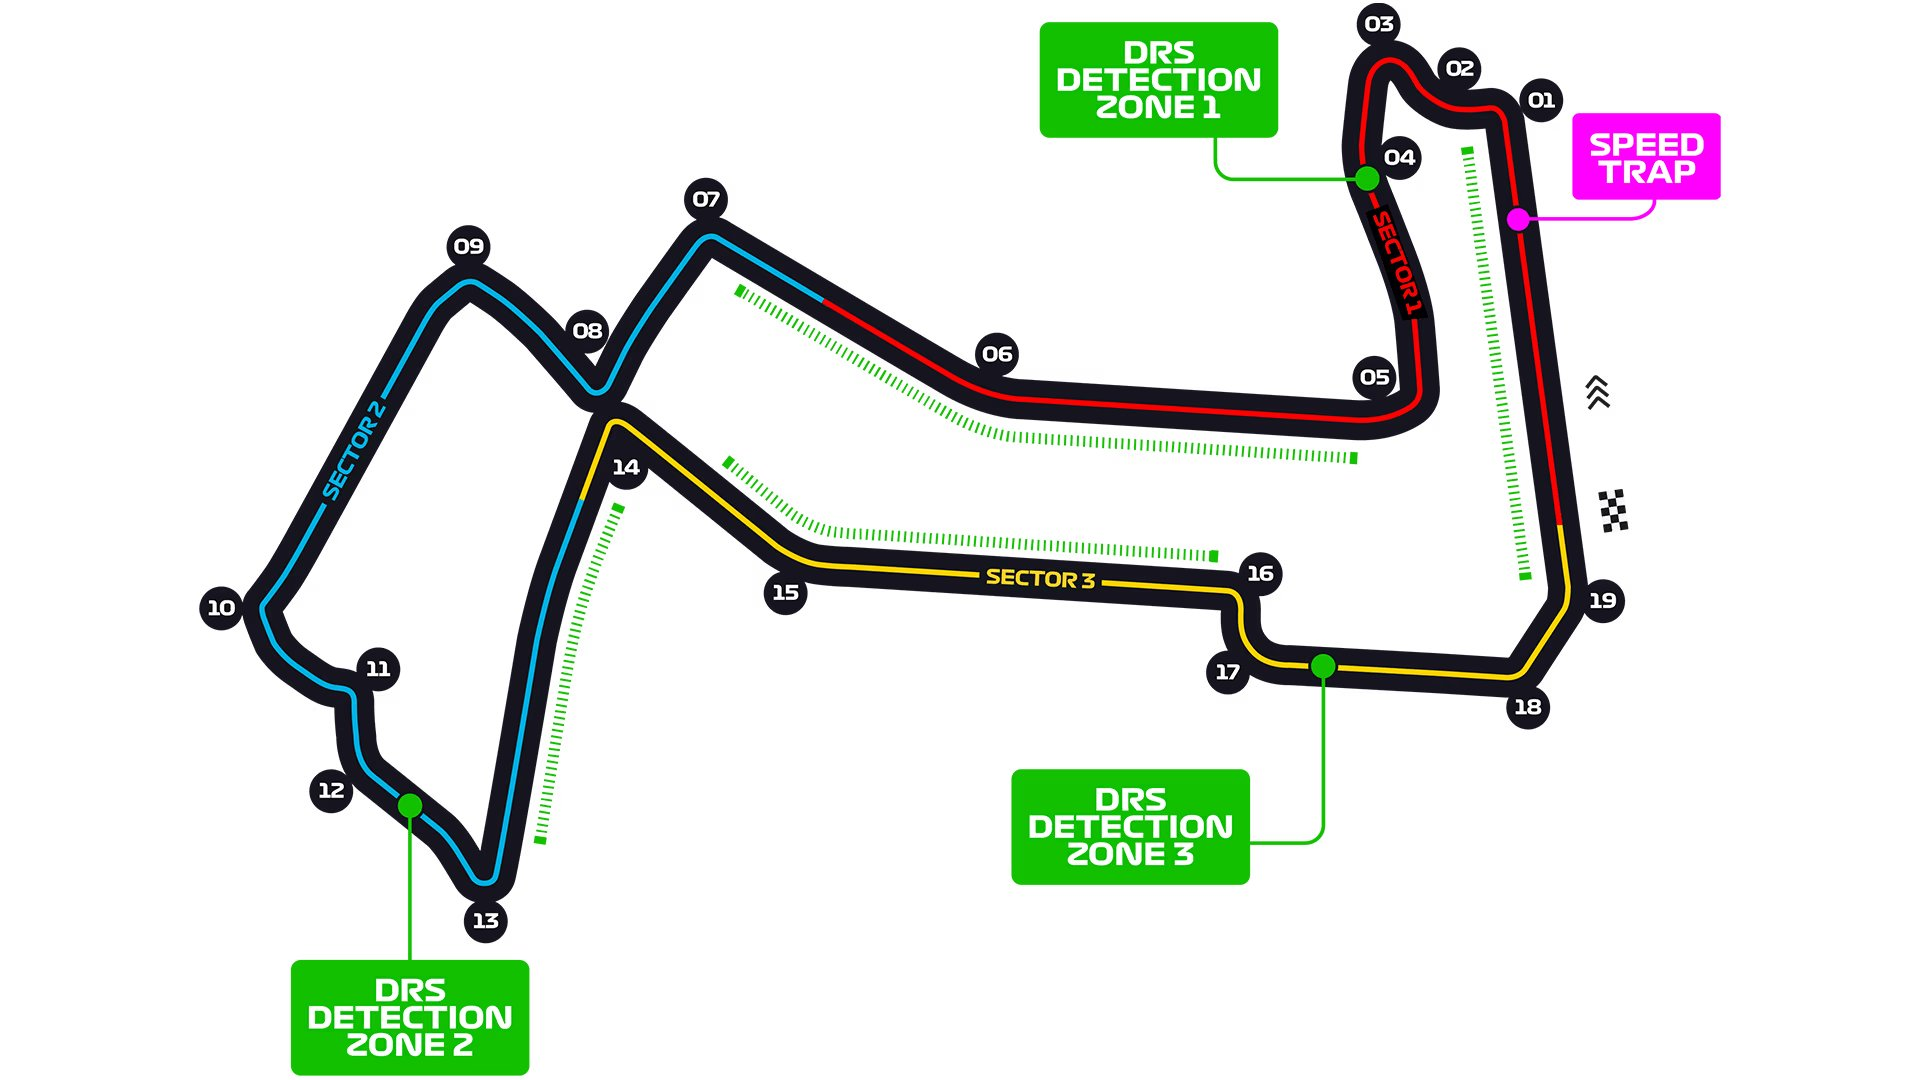
\includegraphics[width=0.75\linewidth]{images/18.Singapore_Circuit.jpg}
\end{figure}

\begin{itemize}
    \item \textbf{Lap Record} : 1:30.984 (2023, Carlos Sainz – Ferrari).
    
    \item \textbf{Number of Corners \& Key Features} : 19 turns (8 right, 11 left). \\
    Demanding street circuit with constant braking and traction zones. \\
    Night race under artificial lighting, with unique atmosphere and track conditions.
    
    \item \textbf{Braking Zones \& Traction} : Very heavy braking into Turns 1, 7 and 14. \\
    Traction out of slow corners is critical, punishing poor rear stability.
    
    \item \textbf{DRS \& Overtaking} : Four DRS zones (main straight, between Turns 5–7, before turn 14 and between Turns 14-16). \\
    Overtaking opportunities limited, mainly into Turn 7.
    
    \item \textbf{Tyre Degradation \& Strategy} : Hot and humid conditions create extreme tyre stress. \\
    Surface evolution is significant and Safety Car probability is high, influencing flexible tyre strategies.
    
    \item \textbf{Weather \& Environment} : High humidity and heat test driver endurance. \\
    Street circuit with little margin for error, walls close at every corner.
\end{itemize}

\textbf{Strategic Summary :} Marina Bay rewards qualifying, car balance in low-speed corners, and precise tyre management under extreme conditions. Track position is usually decisive due to narrow layout and difficulty overtaking.

\subsection{Race Analysis}

\textbf{Date:} 22 September 2024 — 20:00 local time 

\begin{itemize}
    \item \textbf{Qualifying Summary} : \textbf{Pole Position:} Lando Norris (McLaren) – 1:29.525 (new track record). \\
    Grid: Verstappen 2nd, Hamilton 3rd, Russell 4th. \\
    Piastri only 5th, Ferrari trapped in Q3 crash (Leclerc 9th, Sainz 10th).
    
    \item \textbf{Race Summary} : \textbf{Winner:} Lando Norris (McLaren). \\
    \textbf{Podium:} 1. Norris - 2. Verstappen - 3. Piastri. \\
    No Safety Car — first time ever in Singapore GP history. 
    
    \item \textbf{Strategies} : \\ 
    - Norris executed a clean one-stop (medium → hard), perfectly managing tyre degradation despite hot conditions. \\
    - Verstappen mirrored strategy but lacked pace to challenge. \\
    - Piastri delayed first stop, enabling overcut on Mercedes. \\
    - Ferrari split strategies: Leclerc long first stint (37 laps) on mediums before switching to hards, effective for P5. \\
    - Hamilton gambled on softs at the start, forced into early stop (lap 17) — limited to P6. 
    
    \item \textbf{Performance Trends} : \textbf{McLaren} dominant: Norris untouchable, Piastri on podium despite starting 5th. \\
    \textbf{Red Bull} showed solid race pace, but Verstappen couldn’t threaten Norris. \\
    \textbf{Ferrari} recovered well from poor grid positions, Leclerc notably effective on long stint. \\
    \textbf{Mercedes} lacked race pace to compete with McLaren and Ferrari. \\
    \textbf{Aston Martin} (Alonso) maximized potential with P8, Haas scored with Hülkenberg.
    
    \item \textbf{Championship Impact} : \textbf{Drivers:} Verstappen 331 pts, Norris 279, Leclerc 245. \\
    \textbf{Constructors:} McLaren 516, Red Bull 475, Ferrari 441, Mercedes 329.
\end{itemize}

\textbf{Key Takeaway :} Lando Norris achieved his first ever lights-to-flag victory, showcasing McLaren’s superiority in street conditions. Ferrari salvaged strong points with clever strategy, while Mercedes struggled to match rivals.

\subsection{Link \& Takeaway}

\begin{itemize}
    \item Singapore’s stop-start layout rewarded cars with strong low-speed traction and mechanical grip — McLaren’s strength in 2024. \\
    Norris dominated thanks to superior corner exit performance and tyre management in extreme heat.
    \item Ferrari’s strategic creativity (Leclerc’s long first stint) allowed recovery from poor grid positions. 
    \item Mercedes’ lack of rear grip punished them over long stints, while Aston Martin and Haas capitalized on attrition-free race. 
    \item Red Bull showed consistency but not the edge needed to beat McLaren, Verstappen’s P2 minimized losses in the title fight.
    \item With no Safety Car interventions, pure pace and tyre discipline decided the outcome — McLaren prevailed by maximizing its car’s balance in Singapore’s unique conditions.
\end{itemize}

\section{United States Grand Prix}

\subsection{Circuit Analysis}

\textbf{Circuit Name:} Circuit of the Americas (Austin, Texas, USA) \\
\textbf{Length:} 5.513 km - \textbf{Laps:} 56 - \textbf{Total Distance:} 308.405 km

\begin{figure}[H]
    \centering
    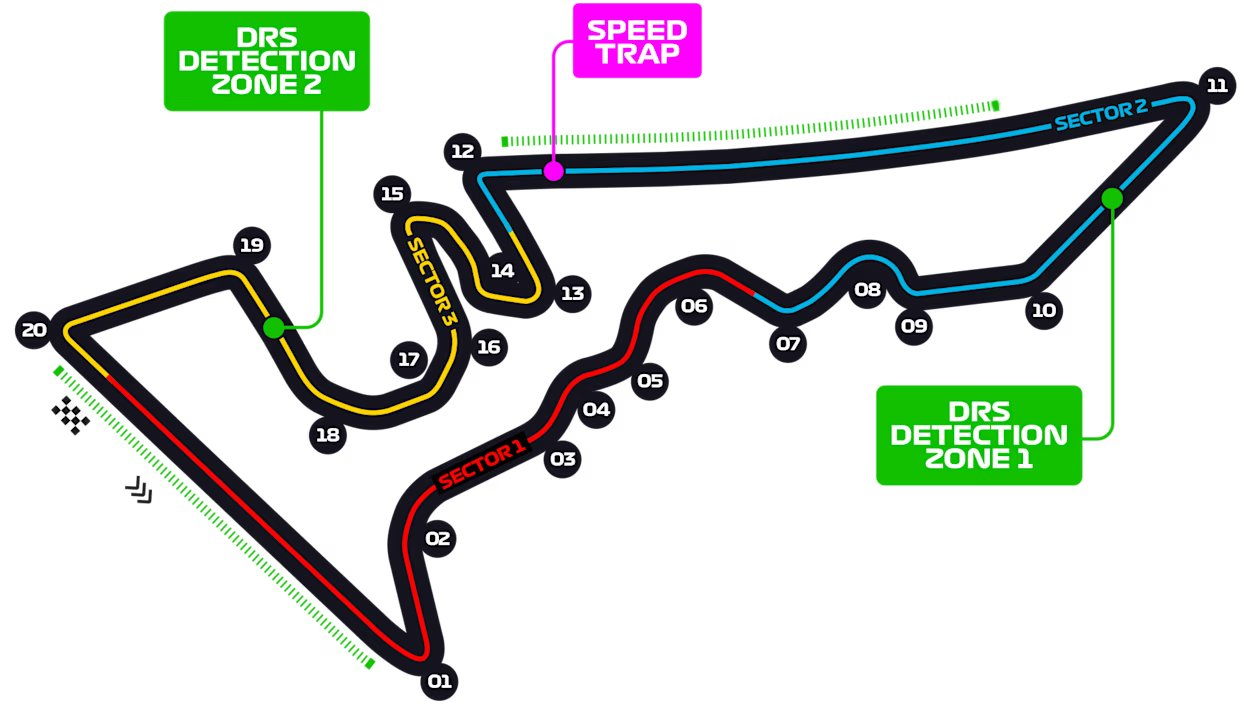
\includegraphics[width=0.75\linewidth]{images/19.United_States_Circuit.jpg}
\end{figure}

\begin{itemize}
    \item \textbf{Lap Record} : 1:32.029 (2019, Valterri Bottas – Red Bull).
    
    \item \textbf{Number of Corners \& Key Features} : 20 turns (8 right, 12 left), highly technical mix of high-speed esses, tight hairpins, and long straights. \\
    Iconic uphill run into Turn 1, wide entry allowing multiple lines. 
    
    \item \textbf{Braking Zones \& Traction} : Heavy braking at Turn 1 and Turn 12. \\
    Rear stability critical for acceleration out of slow corners.
    
    \item \textbf{DRS \& Overtaking} : Two DRS zones (main straight and back straight into Turn 12). \\
    Multiple overtaking opportunities but strong defence possible due to wide track.
    
    \item \textbf{Tyre Degradation \& Strategy} : Medium degradation, high rear wear. \\
    Undercuts very powerful due to long pit exit loss and track layout. \\
    Two-stop strategies most effective.
    
    \item \textbf{Weather \& Environment} : Warm Texan climate, bumpy asphalt. \\
    Circuit demands both aero efficiency and mechanical grip.
\end{itemize}

\textbf{Strategic Summary :} COTA rewards cars with strong straight-line speed, good traction, and ability to manage high-energy corners. Strategy is often defined by the undercut power and defending into Turn 12.

\subsection{Race Analysis}

\textbf{Date:} Sprint : 19 October 2024 - 13:00 local time\\
Race : 20 October 2024 — 14:00 local time 

\begin{itemize}
    \item \textbf{Sprint Qualifying:} \textbf{Pole Position:} Max Verstappen (Reb Bull) - 1:32.833.\\
    Grid : Russell 2nd, Leclerc 3rd, Norris 4th. \\
    Haas surprised with both cars in SQ3 (Hülkenberg P6, Magnussen P8). Piastri eliminated early (P16).
    
    \item \textbf{Sprint Race Summary:} \textbf{Winner:} Max Verstappen (Red Bull). \\
    \textbf{Podium:} 1. Verstappen - 2. Sainz - 3. Norris. \\
    Leclerc P4, Mercedes in points (Russell P5, Hamilton P6), Haas scored (Magnussen P7, Hülkenberg P8). \\
    Piastri finished outside points.
    
    \item \textbf{Qualifying Summary:} \textbf{Pole Position:} Lando Norris (McLaren) – 1:32.330. \\
    Grid : Verstappen 2nd, Sainz 3rd, Leclerc 4th. \\
    Hamilton shock Q1 elimination (P19).
    
    \item \textbf{Race Summary:} \textbf{Winner:} Charles Leclerc (Ferrari) — lights-to-flag dominance after Turn 1 move. \\
    \textbf{Podium:} 1. Leclerc - 2. Sainz - 3. Verstappen. \\
    Norris crossed P3 but penalised 5s for off-track pass, classified P4. \\
    Ferrari celebrated their second 1–2 of the season. \\
    \textbf{Notable incidents:} Hamilton crashed out lap 2. \\
    Lawson (P9) and Colapinto (P10) both scored first career points.
    
    \item \textbf{Strategies:} \\
    - Leclerc: medium → hard (lap 26), flawless execution. \\
    - Sainz: undercut Verstappen between laps 21–25, decisive for P2. \\
    - Verstappen: medium → hard, lacked pace against Ferraris, defended hard vs Norris. \\
    - Norris: extended first stint (lap 31), tried fresher tyres late, penalised for pass. \\
    - Piastri: steady but stuck behind top 4, finished P5. \\
    - Russell: pitlane start + penalty, recovered to P6. \\
    - Ocon: fastest lap on softs but outside top 10, no bonus point.
    
    \item \textbf{Performance Trends:} \textbf{Ferrari} strongest race pace all season, clear 1–2. \\
    \textbf{Red Bull} fast in sprint but weaker in GP, Verstappen forced into defence. \\
    \textbf{McLaren} strong on Saturday but race execution compromised by penalties. \\
    \textbf{Mercedes} mixed: Russell recovered, Hamilton eliminated early. \\
    \textbf{Haas} consistent points, \textbf{Williams} breakthrough with Colapinto, Lawson scored on \textbf{Racing Bulls} debut.
    
    \item \textbf{Championship Impact:} \textbf{Drivers:} Verstappen 354 pts, Norris 297, Leclerc 275. \\
    \textbf{Constructors:} McLaren 544, Red Bull 504, Ferrari 496, Mercedes 344.
\end{itemize}

\textbf{Key Takeaway :} Ferrari delivered a dominant 1–2, with Leclerc in control from Turn 1 and Sainz executing the decisive undercut on Verstappen. McLaren showed raw pace but faltered in race execution, while Red Bull had no answer to Ferrari’s superior tyre life.

\subsection{Link \& Takeaway}

\begin{itemize}
    \item COTA’s wide layout and heavy braking zones favoured Ferrari’s strong traction and straight-line speed. Leclerc’s Turn 1 move set the tone for the race. 
    \item Sainz capitalised on undercut power at Austin to secure Ferrari’s 1–2, showing the team’s sharp race management. 
    \item Verstappen salvaged podiums across sprint and race but showed Red Bull’s vulnerability in tyre longevity compared to Ferrari. 
    \item Norris’ penalty underlined how strict track limits at COTA can reshape results, even in late-race battles. 
    \item Lawson and Colapinto’s points showed how unpredictable COTA can be for midfield teams, with opportunities emerging from attrition and penalties. 
    \item Ferrari’s dominant pace gave them their biggest points haul of the season, reigniting their constructors’ title hopes.
\end{itemize}

\section{Mexican Grand Prix}

\subsection{Circuit Analysis}

\textbf{Circuit Name:} Autódromo Hermanos Rodríguez (Mexico City, Mexico) \\
\textbf{Length:} 4.304 km - \textbf{Laps:} 71 - \textbf{Total Distance:} 305.354 km

\begin{figure}[H]
    \centering
    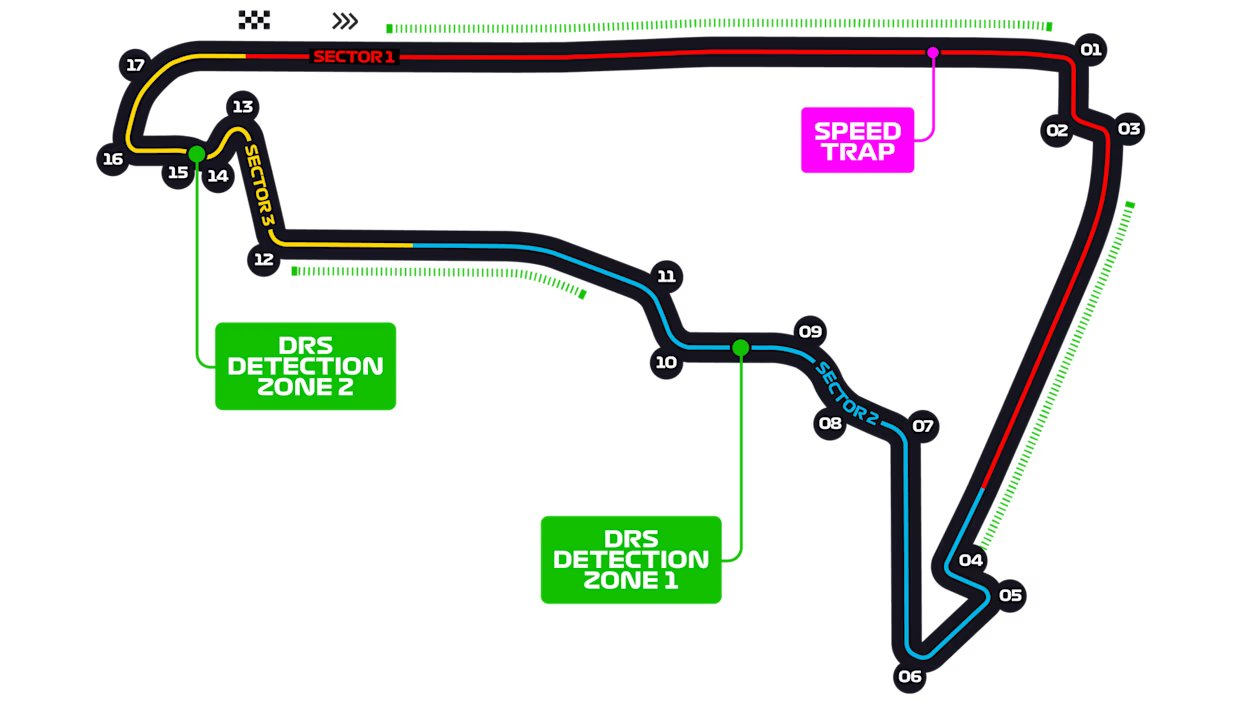
\includegraphics[width=0.75\linewidth]{images/20.Mexico_Circuit.jpg}
\end{figure}

\begin{itemize}
    \item \textbf{Lap Record} : 1:14.758 (2019, Max Verstappen - Red Bull).
    
    \item \textbf{Number of Corners \& Key Features} : 17 turns (10 right, 7 left), mix of long straights and tight technical complexes. \\
    Iconic sections include the long main straight (1.2 km) into Turn 1, and the stadium sector (Turns 12–16) with spectacular crowd atmosphere.
    
    \item \textbf{Braking Zones \& Traction} : Heavy braking into Turn 1 (from 350 km/h to 100 km/h). \\
    Traction critical out of slow corners in the stadium, especially Turn 16 onto the straight.
    
    \item \textbf{DRS \& Overtaking} : Three DRS zones (main straight, between Turns 3–4, and between Turns 11–12). \\
    Turn 1 is the prime overtaking spot, stadium sector allows close racing but little passing.
    
    \item \textbf{Tyre Degradation \& Strategy} : Medium to high wear due to low air density and limited cooling. \\
    Two-stop strategies typical, undercut powerful with long pit lane loss.
    
    \item \textbf{Weather \& Environment} : High altitude (2,240m) reduces engine power and cooling efficiency. \\
    Brakes and tyres face added stress from thin air.
\end{itemize}

\textbf{Strategic Summary :} Mexico demands power unit efficiency under high altitude, strong braking for Turn 1, and tyre management under thermal stress. Track position at the start is crucial due to the long run into Turn 1.

\subsection{Race Analysis}

\textbf{Date:} 27 October 2024 — 14:00 local time 

\begin{itemize}
    \item \textbf{Qualifying Summary} : \textbf{Pole Position:} Carlos Sainz (Ferrari) – 1:15.946. \\
    Grid : Verstappen 2nd, Norris 3rd, Leclerc 4th. \\
    Magnussen P7, Gasly P8 (second consecutive Q3). Piastri and Pérez eliminated in Q1.
    
    \item \textbf{Race Summary} : \textbf{Winner:} Carlos Sainz (Ferrari) — dominant recovery after early loss of lead. \\
    \textbf{Podium:} 1. Sainz - 2. Norris - 3. Leclerc. \\
    Verstappen led the opening laps but penalised twice (20s total) for forcing Norris off track. \\
    Leclerc secured fastest lap on final lap. Hamilton beat Russell for P4 in late Mercedes duel. \\
    
    \item \textbf{Notable Incidents} : \\
    - Lap 1: Gasly causes contact between Tsunoda and Albon → Safety Car. Albon + Tsunoda retire. \\
    - Verstappen penalised (10s for Turn 4 squeeze, 10s for Turn 8 move vs Norris). \\
    - Lap 63: Leclerc slides wide at final corner, Norris overtakes for P2. \\
    - Alonso retires (brakes). \\
    - Colapinto penalised for contact with Lawson. \\
    - Pérez penalised for incorrect grid position.
    
    \item \textbf{Strategies} : \\
    - Sainz: medium → hard (lap 25), fastest overall management. \\
    - Norris: medium → hard, pressured Leclerc late and seized P2 after his error. \\
    - Leclerc: medium → hard, strong but lost P2 under pressure. \\
    - Verstappen: early stop to serve penalty, dropped to P15, recovered only to P6. \\
    - Mercedes: medium → hard, close intra-team battle, Hamilton prevailed. \\
    - Haas: strong pace all weekend, Magnussen P7, Hülkenberg P9. \\
    - Piastri: started P17, recovered to P8 with aggressive stints.
    
    \item \textbf{Performance Trends} : \textbf{Ferrari} fastest overall (pole + win + fastest lap). \\
    \textbf{McLaren} competitive but lacked straight-line defence, Norris maximised recovery. \\
    \textbf{Red Bull} inconsistent, Verstappen’s penalties costly, Pérez invisible at home GP. \\
    \textbf{Mercedes} strong in race pace, but behind Ferrari/McLaren.
    
    \item \textbf{Championship Impact} : \textbf{Drivers:} Verstappen 362 pts, Norris 315, Leclerc 291. \\
    \textbf{Constructors:} McLaren 566, Ferrari 537 (+1), Red Bull 512 (-1), Mercedes 366.
\end{itemize}

\textbf{Key Takeaway :} Carlos Sainz controlled Mexico with Ferrari’s superior pace, while Verstappen’s penalties exposed Red Bull’s growing weaknesses. Norris capitalised late for P2, Leclerc salvaged P3 + fastest lap, and Mercedes showed solid but unspectacular form. Haas confirmed progress with both cars in points.

\subsection{Link \& Takeaway}

\begin{itemize}
    \item Mexico’s long run to Turn 1 reshaped the race start — Verstappen briefly led but couldn’t contain Ferrari’s pace. 
    \item Ferrari’s strength in medium-to-hard stints secured victory, Sainz maximised track position and tyre life. 
    \item Verstappen’s aggressive defence and penalties symbolised Red Bull’s desperation under pressure. 
    \item Norris showed McLaren’s persistence with a late overtake on Leclerc, but Ferrari clearly had the upper hand. 
    \item High altitude punished power units and cooling, teams with efficient aero and tyre control thrived, notably Ferrari and Haas. 
    \item With this win, Ferrari reignited the constructors’ title fight, closing the gap to McLaren and Red Bull with just four races left.
\end{itemize}

\section{São Paulo Grand Prix}

\subsection{Circuit Analysis}

\textbf{Circuit Name:} Autódromo José Carlos Pace (Interlagos, São Paulo, Brazil) \\
\textbf{Length:} 4.309 km - \textbf{Laps:} 71 - \textbf{Total Distance:} 305.879 km

\begin{figure}[H]
    \centering
    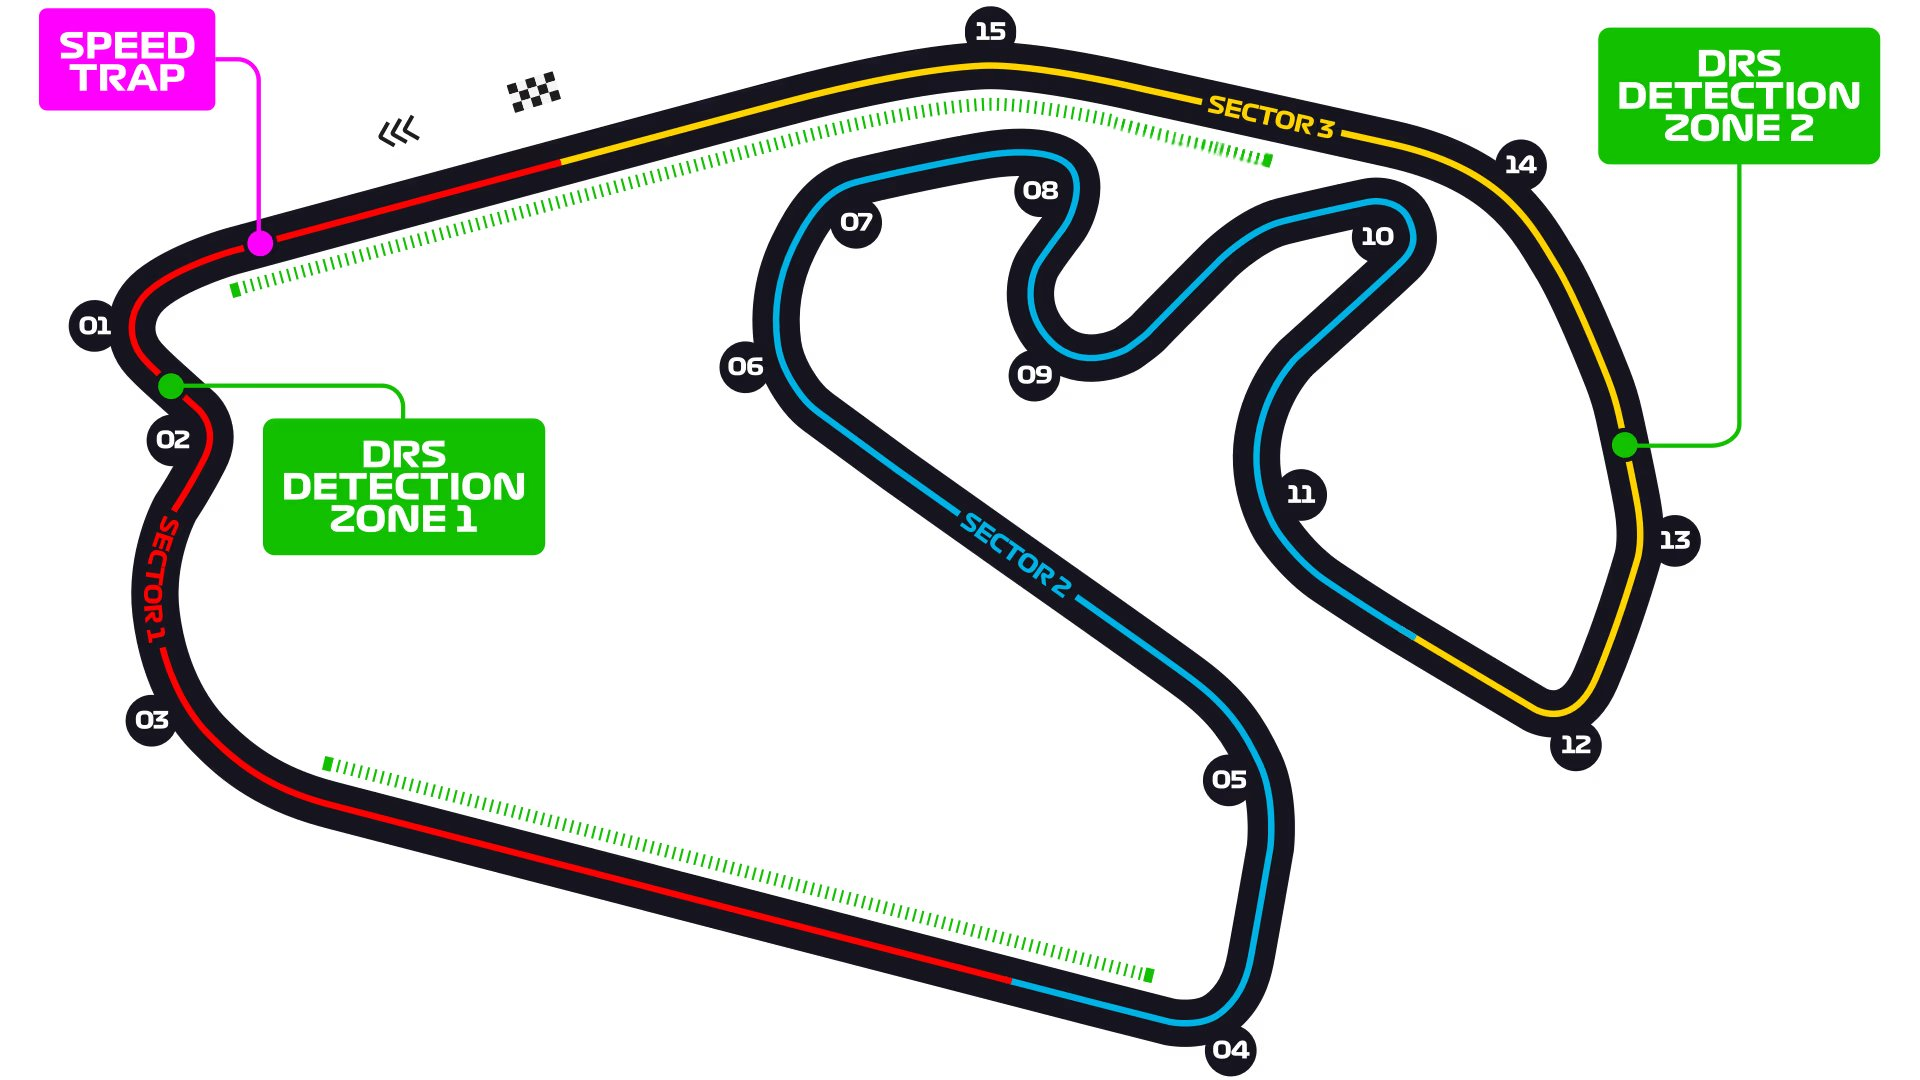
\includegraphics[width=0.75\linewidth]{images/21.Brazil_Circuit.jpg}
\end{figure}

\begin{itemize}
    \item \textbf{Lap Record} : 1:07.281 (2018, Lewis Hamilton – Mercedes).
    
    \item \textbf{Number of Corners \& Key Features} : 15 turns (5 right, 10 left). \\
    Counter-clockwise layout, famous for “Senna S” (Turns 1–2) and long uphill straight. \\
    High altitude + bumpy surface increase mechanical stress.
    
    \item \textbf{Braking Zones \& Traction} : Turn 1 (Senna S) heavy braking, prime overtaking zone. \\
    Traction critical at Juncão (Turn 12) leading to full-throttle run to finish line.
    
    \item \textbf{DRS \& Overtaking} : Two DRS zones (main straight and between Turns 3–4). \\
    Turn 1 and Turn 4 are the main overtaking opportunities.
    
    \item \textbf{Tyre Degradation \& Strategy} : High degradation due to track abrasiveness and elevation. \\
    Two-stop strategy typical, though weather chaos often dictates.
    
    \item \textbf{Weather \& Environment} : São Paulo notorious for sudden rain showers. \\
    Thin air reduces engine power, unpredictable conditions play major role.
\end{itemize}

\textbf{Strategic Summary :} Interlagos combines altitude challenges, mixed-speed corners, and unpredictable weather. Start and tyre strategy are critical; race often decided by timing of pitstops and Safety Cars.

\subsection{Race Analysis}

\textbf{Date:} Sprint : 2 November 2024 - 11:00 local time\\
Race : 3 November 2024 — 12:00 local time 

\begin{itemize}
    \item \textbf{Sprint Qualifying:} \textbf{Pole Position:} Oscar Piastri (McLaren) - 1:08.899.\\
    Grid : Norris 2nd, Leclerc 3rd, Verstappen 4th.
    
    \item \textbf{Sprint Summary} : \textbf{Winner:} Lando Norris (McLaren). \\
    \textbf{Podium:} 1. Norris - 2. Piastri - 3. Leclerc. \\
    Verstappen penalised 5s → dropped to P4.
    
    \item \textbf{Qualifying Summary} : Chaotic wet session with 5 red flags. \\
    \textbf{Pole Posision:} Lando Norris (McLaren) – 1:23.405. \\
    Grid : Russell 2nd, Tsunoda 3rd, Ocon 4th. \\
    Lawson P5, Leclerc P6. Verstappen only P12, dropped to P17 with engine penalty. Albon crashed in Q3 → DNS.
    
    \item \textbf{Race Summary} : \textbf{Winner:} Max Verstappen (Red Bull) — stunning recovery from P17. \\
    \textbf{Podium:} 1. Verstappen - 2. Ocon - 3. Gasly. \\
    Race started under rain, multiple Safety Cars and a red flag. \\
    Russell led first 28 laps, then Ocon/Gasly stayed out in worsening rain and temporarily led. \\
    After restart, Verstappen passed Ocon at Turn 1 (lap 43) and pulled away, also taking fastest lap. \\
    Norris struggled, finished only P6. Double Alpine podium, first since Spain 1997 with two French drivers.
    
    \item \textbf{Notable Incidents} : \\
    - Lap 1: Stroll spun off during formation, DNS. \\
    - Lap 27: Heavy rain → mass pitstops, Ocon and Gasly stayed out. \\
    - Lap 30: Colapinto big crash → red flag. \\
    - Lap 38: Sainz crashed → Safety Car. \\
    - Lap 43: Verstappen overtakes Ocon for the lead. \\
    - Piastri + Bearman penalised 10s for contacts. Hülkenberg disqualified after receiving external help.
    
    \item \textbf{Strategies} : \\
    - Verstappen: intermediate → wet → slicks, perfectly timed, + fastest lap. \\
    - Ocon/Gasly: bold gamble staying out before red flag, secured podiums. \\
    - Mercedes: Russell led early but faded, finished P4; Hamilton P10 after recovery. \\
    - McLaren: Norris lost momentum with off-track moment, P6. Piastri penalised, P8. \\
    - Ferrari: Leclerc P5 solid, Sainz retired in crash. \\
    - Racing Bulls: Tsunoda P7, Lawson P9. \\
    - Haas: Bearman penalised, P12; Hülkenberg DSQ.
    
    \item \textbf{Performance Trends} : \textbf{Red Bull} back on top with Verstappen’s comeback. \\
    \textbf{Alpine} revived with double podium, showing opportunistic strategy. \\
    \textbf{McLaren} lacked composure in chaos, Ferrari steady but unspectacular. \\
    \textbf{Mercedes} strong start but couldn’t sustain. \\
    \textbf{Williams} collapsed after Albon DNS and Colapinto crash. 
    
    \item \textbf{Championship Impact} : \textbf{Drivers:} Verstappen 393 pts, Norris 331, Leclerc 307. \\
    \textbf{Constructors:} McLaren 593, Ferrari 557, Red Bull 544, Mercedes 382. \\
    Verstappen can clinch title at next race in Las Vegas.
\end{itemize}

\textbf{Key Takeaway :} Verstappen produced one of his greatest wins, storming from P17 to victory in chaotic São Paulo conditions. Alpine shocked the paddock with a double podium, McLaren faltered, and Mercedes/Ferrari lacked decisive pace. Championship battle tightened in constructors, but Verstappen now holds the drivers’ crown within reach.

\subsection{Link \& Takeaway}

\begin{itemize}
    \item Interlagos delivered another chaotic thriller: rain, Safety Cars, red flag, and late drama. 
    \item Verstappen showcased racecraft and adaptability, turning a P17 start into a commanding win. 
    \item Alpine’s opportunism rewarded with a historic French double podium, a rare highlight in their season. 
    \item McLaren slipped under pressure, Ferrari stayed consistent, Mercedes missed podium chance. 
    \item The result leaves Verstappen with one hand on the drivers’ trophy, while constructors’ title fight remains wide open. 
\end{itemize}

\section{Las Vegas Grand Prix}

\subsection{Circuit Analysis}

\textbf{Circuit Name:} Las Vegas Strip Circuit (Las Vegas, United States) \\
\textbf{Length:} 6.120 km - \textbf{Laps:} 50 - \textbf{Total Distance:} 305.880 km

\begin{figure}[H]
    \centering
    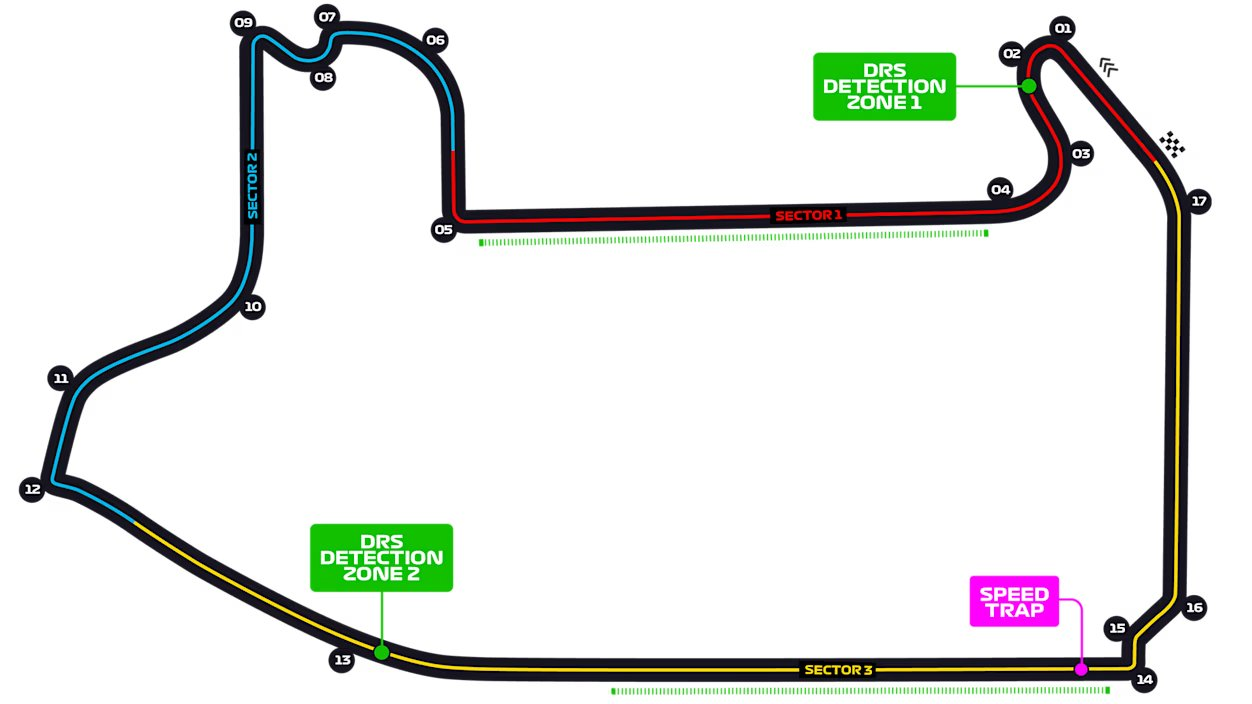
\includegraphics[width=0.75\linewidth]{images/22.Las_Vegas_Circuit.jpg}
\end{figure}

\begin{itemize}
    \item \textbf{Lap Record} : 1:32.726 (2023, Charles Leclerc - Ferrari).
    
    \item \textbf{Number of Corners \& Key Features} : 17 turns (6 right, 11 left). \\
    The layout includes a 1.9 km straight along the Strip, heavy braking zones, and long traction phases. \\
    Street circuit, wide but slippery, with bumps and cold asphalt conditions at night.
    
    \item \textbf{Braking Zones \& Traction} : Turns 1, 5, and 14 are the heaviest braking points. \\
    Grip difficult to find in cold conditions, traction at corner exits is crucial.
    
    \item \textbf{DRS \& Overtaking} : Two DRS zones: between Turns 4–5 and before Turn 14. \\
    Main overtaking opportunities into Turn 1 and Turn 14.
    
    \item \textbf{Tyre Degradation \& Strategy} : Night temperatures make tyre warm-up difficult. \\
    Surface abrasive, causing high degradation despite cool climate. \\
    Two-stop race strategies prevailed.
    
    \item \textbf{Weather \& Environment} : Cold Nevada nights (below 15°C). \\
    Low grip and tyre temperature management are defining factors. \\
    Unpredictable conditions make safety cars likely.
\end{itemize}

\textbf{Strategic Summary :} The Las Vegas Strip Circuit is defined by long straights, cold conditions, and high tyre wear. Mercedes unlocked grip where rivals failed, controlling the weekend.

\subsection{Race Analysis}

\textbf{Date:} 23 November 2024 — 22:00 local time

\begin{itemize}
    \item \textbf{Qualifying Summary} : \textbf{Pole Position:} George Russell (Mercedes) – 1:32.312 (new track record). \\
    Grid: Sainz 2nd, Gasly 3rd, Leclerc 4th. \\
    Hamilton only P10, recovered from a tough qualifying. Colapinto crashed heavily in Q2 (50g impact), started from pitlane.
    
    \item \textbf{Race Summary} : \textbf{Winner:} George Russell (Mercedes). \\
    \textbf{Podium:} 1. Russell - 2. Hamilton - 3. Sainz. \\
    Mercedes secured its 60th 1–2 finish in F1 history. \\
    Verstappen clinched his fourth World Championship despite finishing 5th, ahead of Norris (P6). \\
    \textbf{Technical issues:} Gasly (engine, lap 15), Albon (turbo, lap 25).
    
    \item \textbf{Strategies} : \\
    - Mercedes (Russell, Hamilton): two-stop (Medium–Hard–Medium), optimal under cold conditions. \\
    - Ferrari: Sainz P3, Leclerc P4 after intra-team strategy clash (Sainz ignored team orders). \\
    - Red Bull: Verstappen conservative, secured title ahead of Norris. Pérez salvaged P10. \\
    - McLaren: Norris struggled with grip, salvaged fastest lap on final lap, Piastri penalised, P7. \\
    - Haas: Hülkenberg strong P8; Magnussen just outside points. \\
    - Racing Bulls: Tsunoda P9, Lawson faded to P16. \\
    - Williams: Colapinto finished P14 after pitlane start, Albon retired.
    
    \item \textbf{Performance Trends} : \textbf{Mercedes} finally dominated: Russell untouchable, Hamilton “Driver of the Day”. \\
    \textbf{Ferrari} solid podium presence but suffered internal friction. \\
    \textbf{Red Bull} less competitive, but Verstappen achieved main target: title secured. \\
    \textbf{McLaren} off the pace on cold asphalt, limiting Norris’ comeback. \\
    \textbf{Alpine}’s high of São Paulo collapsed with Gasly’s DNF and Ocon only P17.
    
    \item \textbf{Championship Impact} : \textbf{Drivers:} Verstappen 403 pts (Champion), Norris 340, Leclerc 319. \\
    \textbf{Constructors:} McLaren 608, Ferrari 584, Red Bull 555, Mercedes 425. \\
    Constructors’ battle remains fierce: McLaren vs Ferrari vs Red Bull.
\end{itemize}

\textbf{Key Takeaway :} Mercedes conquered Las Vegas with a dominant 1–2, Russell victorious under the lights. Ferrari consistent, Red Bull focused on sealing Verstappen’s title, and McLaren underperformed but stayed in the Constructors’ lead. The championship is settled for Verstappen, but the fight between McLaren, Ferrari, and Red Bull heads until the final of the season.

\subsection{Link \& Takeaway}

\begin{itemize}
    \item Mercedes adapted best to low temperatures and tricky grip, unlocking tyre performance. 
    \item Ferrari showed pace but internal strategy disputes hindered them. 
    \item Verstappen’s cautious but efficient race secured his fourth consecutive title. 
    \item McLaren lacked consistency in cold conditions, losing ground despite fastest lap. 
    \item The Constructors’ Championship remains undecided. 
\end{itemize}

\section{Qatar Grand Prix}

\subsection{Circuit Analysis}

\textbf{Circuit Name:} Losail International Circuit (Lusail, Qatar) \\
\textbf{Length:} 5.419 km - \textbf{Laps:} 57 - \textbf{Total Distance:} 308.611 km

\begin{figure}[H]
    \centering
    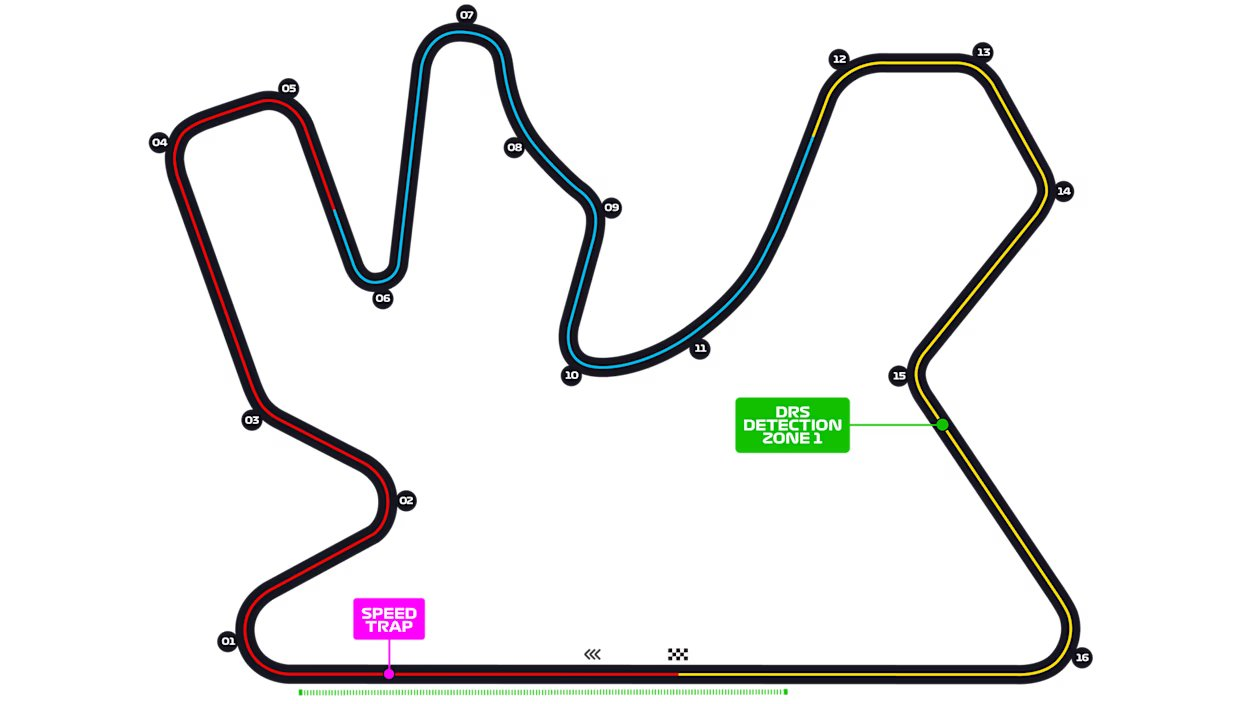
\includegraphics[width=0.75\linewidth]{images/23.Qatar_Circuit.jpg}
\end{figure}

\begin{itemize}
    \item \textbf{Lap Record} : 1:20.827 (2021, Lewis Hamilton - Mercedes).

    \item \textbf{Number of Corners \& Key Features} : 16 turns (10 right, 6 left). \\
    Fast, flowing track with medium–high downforce demand. Long straights combined with technical sequences.
    
    \item \textbf{Braking Zones \& Traction} : Main braking into Turn 1. \\
    High-speed corners put stress on front tyres, with traction key in final sector.

    \item \textbf{DRS \& Overtaking} : One long DRS zone on the main straight. \\
    Overtaking possible in Turn 1, otherwise difficult due to narrow track.

    \item \textbf{Tyre Degradation \& Strategy} : Hot conditions typically strain tyres, but night race reduces temperatures. \\
    Still, abrasive surface leads to high wear: multi-stop strategies usual.

    \item \textbf{Weather \& Environment} : Night race under floodlights. \\
    Air temperature cooler but track remains abrasive and dusty, reducing grip.
\end{itemize}

\textbf{Strategic Summary :} Lusail rewards aerodynamic balance and tyre preservation. Track evolution significant, safety cars often influence strategy.

\subsection{Race Analysis}

\textbf{Date:} Sprint : 30 November 2024 - 17:00 local time\\
Race : 1 December 2024 — 19:00 local time 

\begin{itemize}
    \item \textbf{Sprint Qualifying:} \textbf{Pole Position:} Lando Norris (McLaren) - 1:21.012.\\
    Grid : Russell 2nd, Piastri 3rd, Sainz 4th.

    \item \textbf{Sprint Summary} : \textbf{Winner:} Oscar Piastri (McLaren). \\
    \textbf{Podium}: 1. Piastri - 2. Norris - 3. Russell. \\
    Norris slowed deliberately at the end to give Piastri the win in return for São Paulo. Haas scored big with Hülkenberg P7. Verstappen only 8th. McLaren strengthened constructors’ lead.

    \item \textbf{Qualifying Summary} : \textbf{Fastest Lap in Q3:} Max Verstappen (Red Bull) – 1:20.520. \\
    \textbf{Pole Position:} George Russell (Mercedes) – 1:20.575 (new track record). \\
    Grid: Verstappen 2nd, Norris 3rd, Piastri 4th, Leclerc 5th. \\
    Max Verstappen, who finished 1st during the qualifications, was penalised of on grid place for impeding.

    \item \textbf{Race Summary} : \textbf{Winner:} Max Verstappen (Red Bull). \\
    \textbf{Podium:} 1. Verstappen - 2. Leclerc - 3. Piastri. \\
    Norris dropped to P10 after 10s stop-and-go penalty under double yellow, but claimed fastest lap. \\
    Zhou scored Kick Sauber’s first points of the season (P8). \\
    \textbf{Multiple incidents}: Ocon and Colapinto out at start, Stroll–Albon clash, Pérez retired with clutch issues, Hülkenberg crashed out lap 39.

    \item \textbf{Strategies} : \\
    - Red Bull: Verstappen flawless, benefitted from Safety Car pit stop. Pérez retired. \\
    - Ferrari: Leclerc solid P2, Sainz P6. \\
    - McLaren: Piastri strong P3, Norris sabotaged by penalty but fastest lap. \\
    - Mercedes: Russell P4 despite penalty, Hamilton only P12 after drive-through. \\
    - Alpine: Gasly excellent P5, Ocon retired at start. \\
    - Kick Sauber: Zhou P8, first points in 2024. 

    \item \textbf{Performance Trends} : \textbf{Red Bull} back on form with Verstappen dominant.\\
    \textbf{Ferrari} consistent, Leclerc under pressure from Piastri. \\
    \textbf{McLaren} still competitive but less dominant. \\
    \textbf{Mercedes} strong in quali but inconsistent in race.\\
    \textbf{Alpine} revived thanks to Gasly. \\
    \textbf{Kick Sauber} celebrated breakthrough points.

    \item \textbf{Championship Impact} : \\
    \textbf{Drivers:} Verstappen 429 pts (Champion), Norris 349, Leclerc 341. \\
    \textbf{Constructors:} McLaren 640, Ferrari 619, Red Bull 581, Mercedes 446. \\
    Abu Dhabi will decide Constructors’ title between McLaren and Ferrari.
\end{itemize}

\textbf{Key Takeaway :} Verstappen dominated under the lights of Lusail. Gasly starred for Alpine, Zhou delivered Kick Sauber’s long-awaited points, and penalties shaped Norris’ and Hamilton’s races. The championship finale at Abu Dhabi is set up for a McLaren vs Ferrari showdown.

\subsection{Link \& Takeaway}

\begin{itemize}
    \item Verstappen proved Red Bull still has sharp teeth, dominating despite title already secured. 
    \item Ferrari stayed in the fight: Leclerc maximised podium points. 
    \item McLaren’s teamwork in the Sprint contrasted with Norris’ penalty in the GP. 
    \item Alpine and Gasly shone, Kick Sauber finally off the mark thanks to Zhou. 
    \item The Constructors’ title will be decided in Abu Dhabi, 21 points between McLaren and Ferrari. 
\end{itemize}

\section{Abu Dhabi Grand Prix}

\subsection{Circuit Analysis}

\textbf{Circuit Name:} Yas Marina Circuit (Abu Dhabi, United Arab Emirates) \\
\textbf{Length:} 5.281 km - \textbf{Laps:} 58 - \textbf{Total Distance:} 306.183 km

\begin{figure}[H]
    \centering
    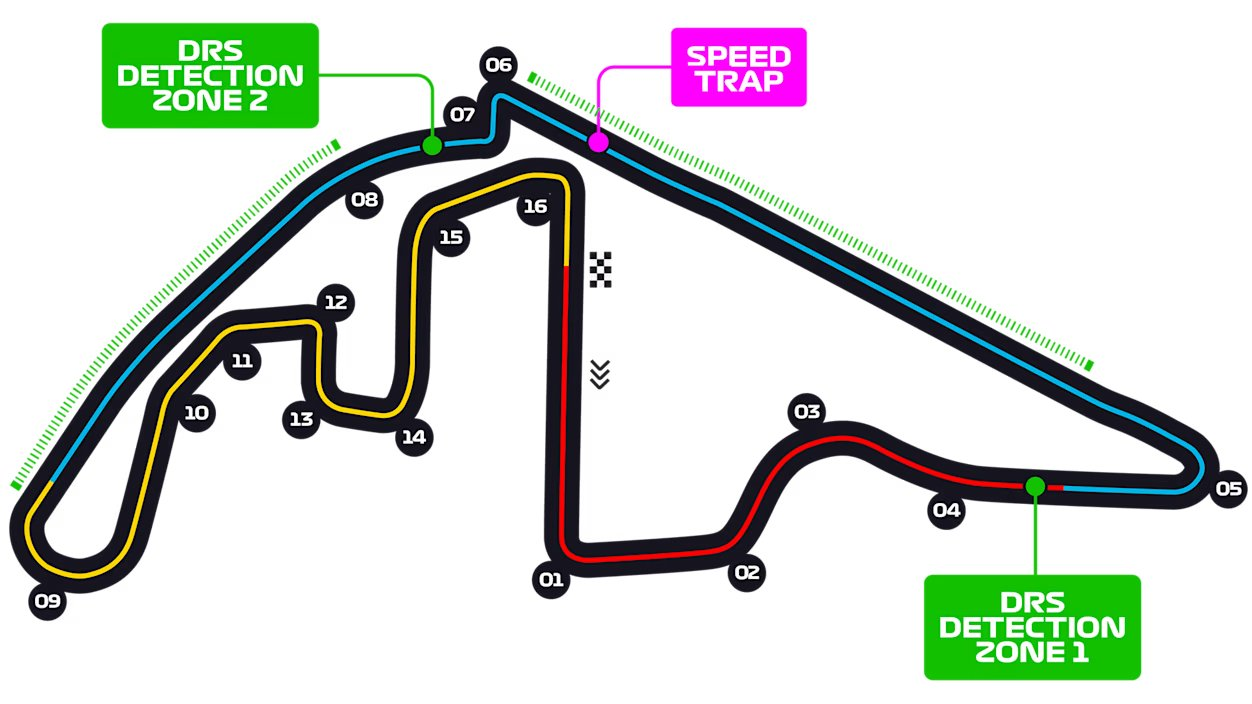
\includegraphics[width=0.75\linewidth]{images/24.Abu_Dhabi_Circuit.jpg}
\end{figure}

\begin{itemize}
    \item \textbf{Lap Record} : 1:23.445 (2023, Max Verstappen – Red Bull). 

    \item \textbf{Number of Corners \& Key Features} : 16 turns (9 right, 7 left). \\
    Features two long straights with heavy braking (Turns 6 and 9), plus a technical third sector. 
    The track layout was revised in 2021 to improve overtaking.

    \item \textbf{Braking Zones \& Traction} : Turn 6 and Turn 9 are prime overtaking zones, requiring strong braking stability. \\
    Sector 3 demands traction and downforce for slow corners leading onto the main straight.

    \item \textbf{DRS \& Overtaking} : Two DRS zones (post-Turn 5 chicane and between Turns 8 and 9). \\
    Overtaking remains challenging but possible with strong exit speed.

    \item \textbf{Tyre Degradation \& Strategy} : Low to medium degradation thanks to smooth asphalt. \\
    One-stop strategies common, but safety cars can shuffle tactics.

    \item \textbf{Weather \& Environment} : Twilight-to-night race under floodlights. \\
    Track temperature drops during the race, aiding tyre management but complicating balance.
\end{itemize}

\textbf{Strategic Summary :} Yas Marina requires aerodynamic efficiency, braking stability, and tyre consistency. The shifting track conditions add complexity to race strategy.

\subsection{Race Analysis}

\textbf{Date:} 8 December 2024 — 17:00 local time 

\begin{itemize}
    \item \textbf{Qualifying Summary} : \textbf{Pole Position:} Lando Norris (McLaren) – 1:22.595 (new track record). \\
    Grid: Piastri 2nd, Sainz 3rd, Verstappen 4th. \\
    Leclerc penalised for power unit change (P19 start). \\
    Hülkenberg dropped from P4 to P7 for pitlane infraction.

    \item \textbf{Race Summary} : \textbf{Winner:} Lando Norris (McLaren) — sealing McLaren’s Constructors’ title. \\
    \textbf{Podium:} 1. Norris - 2. Sainz - 3. Leclerc. \\
    \textbf{Notable incidents:} Verstappen collided with Piastri at Turn 1 (10s penalty, finished P6). Piastri penalised for clash with Colapinto (P10). \\
    Pérez retired lap 1. Bottas and Colapinto also DNFs. Hamilton (hard tyre start) charged from P16 to P4 in his Mercedes farewell.

    \item \textbf{Strategies} : \\
    - McLaren: Norris flawless, Piastri compromised by contact + penalty. \\
    - Ferrari: Sainz P2 (last race with Ferrari), Leclerc P3 from P19 after stunning comeback. \\
    - Mercedes: Hamilton emotional P4 in last race with Mercedes, Russell P5. \\
    - Red Bull: Verstappen salvaged P6 despite penalty, Pérez retired immediately. \\
    - Alpine: Gasly P7 secured Alpine P6 in Constructors’. \\
    - Haas: Hülkenberg P8 solid, Magnussen P16 but fastest lap. \\
    - Alpine rookie debut: Jack Doohan P15, steady first race.

    \item \textbf{Performance Trends} : \textbf{McLaren} dominant with Norris’ pole-to-win.\\
    \textbf{Ferrari} maximised points with both cars on podium. \\
    \textbf{Mercedes} ended strongly with Hamilton’s charge. \\
    \textbf{Red Bull} struggled: Verstappen penalised, Pérez DNF. \\
    \textbf{Alpine} defended crucial P6 in Constructors’.\\
    \textbf{Haas} again competitive with Hülkenberg and fastest lap for Magnussen.

    \item \textbf{Championship Impact} : \\
    \textbf{Drivers:} Verstappen 437 pts (Champion), Norris 374, Leclerc 356. \\
    \textbf{Constructors:} McLaren 666 (Champion), Ferrari 652, Red Bull 589, Mercedes 468. \\
    McLaren clinched first Constructors’ title since 1998.
\end{itemize}

\textbf{Key Takeaway :} Lando Norris dominated Abu Dhabi to crown McLaren Constructors’ Champions for the first time in 26 years. Ferrari’s double podium fell just short, Verstappen ended season on a muted note, while Hamilton delivered a farewell masterclass for Mercedes. Alpine clinched P6 in the standings, Zhou secured Kick Sauber’s first points season since 2022. The 2024 finale sealed a historic McLaren resurgence.

\subsection{Link \& Takeaway}

\begin{itemize}
    \item McLaren sealed their first Constructors’ title since 1998 with a flawless weekend led by Norris. 
    \item Ferrari fought valiantly, but Leclerc’s comeback and Sainz’s podium couldn’t overturn the deficit. 
    \item Verstappen penalised and Pérez retired: Red Bull ended season below expectations. 
    \item Hamilton signed off his Mercedes career with a remarkable recovery drive to P4. 
    \item Alpine’s Gasly defended hard to secure P6 in Constructors’, Haas showed flashes with Hülkenberg and Magnussen. 
    \item Abu Dhabi 2024 will be remembered as the race where McLaren returned to the summit of Formula 1.
\end{itemize}



\section*{Season Conclusion}

\subsection*{General Trends}

The 2024 Formula 1 season was marked by a monumental shift in the power of the Constructors' Championship.
After years of domination by Mercedes and Red Bull, McLaren became the new standard and they won their first Constructors' Title since 1998.
Ferrari displayed consistency and competitiveness throughout the year, while Red Bull suffered from strategic and reliability issues despite Verstappen conquering his fourth consecutive Drivers' Crown. 
Mercedes showed flashes of pace, but inconsistency did not allow for any challenge toward to the top. 
The battle remained intense in the midfield, with Alpine, Haas, and Racing Bulls all fighting for crucial points until the very final race.

\subsection*{Surprises and Highlights}

\begin{itemize}
    \item \textbf{McLaren Resurgence:} Lando Norris achieved four victories and multiple pole positions, supported by Oscar Piastri’s strong season, making McLaren the reference team of 2024.
    \item \textbf{Ferrari’s Consistency:} Charles Leclerc delivered remarkable comebacks (notably Abu Dhabi) and Carlos Sainz closed his Ferrari chapter with steady podiums, giving the team its best campaign in years.
    \item \textbf{Red Bull’s Decline:} While Verstappen secured the Drivers’ title early, the team struggled with tyre wear, strategy missteps, and Sergio Pérez’s lack of competitiveness.
    \item \textbf{Hamilton’s Farewell:} Lewis Hamilton ended his Mercedes era with memorable drives, preparing for a historic move to Ferrari in 2025.
    \item \textbf{Midfield Surprises:} Pierre Gasly’s late-season heroics secured Alpine P6 in the standings. Haas showed progress with Nico Hülkenberg’s qualifying performances and Magnussen’s fastest lap in Abu Dhabi. 
    \item \textbf{Rookies on Stage:} Jack Doohan debuted for Alpine, Liam Lawson and Franco Colapinto scored appearances, while Arthur Leclerc made headlines with his FP1 participation.
\end{itemize}

\subsection*{Team-by-Team Summary}

\begin{itemize}
    \item \textbf{McLaren (Champions, 666 pts):} The revelation of 2024. Norris emerged as Verstappen’s main challenger, while Piastri consolidated McLaren’s return to the top.
    \item \textbf{Ferrari (2nd, 652 pts):} Consistent and fast, but just short of the Constructors’ crown. Leclerc’s form was outstanding, Sainz reliable until his farewell.
    \item \textbf{Red Bull (3rd, 589 pts):} Verstappen dominated individually but Pérez’s poor results cost them dearly. Strategic weaknesses were exposed.
    \item \textbf{Mercedes (4th, 468 pts):} A year of transition. Russell consistent, Hamilton brilliant in moments, but overall lack of pace prevented title contention.
    \item \textbf{Aston Martin (5th, 94 pts):} Alonso continued to extract results, but the car regressed compared to 2023. Stroll failed to deliver significant points.
    \item \textbf{Alpine (6th, 65 pts):} Gasly carried the team with key points late in the season. Ocon’s departure and Doohan’s debut marked a changing era.
    \item \textbf{Haas (7th, 58 pts):} Solid step forward. Hülkenberg competitive in qualifying, Magnussen opportunistic. Midfield progress clear.
    \item \textbf{Racing Bulls (8th, 46 pts):} Tsunoda dependable, Ricciardo underperformed before Lawson’s chance. A team in search of identity.
    \item \textbf{Williams (9th, 17 pts):} Albon remained the leading force, Colapinto debuted with promise. Still lacking consistency to fight higher.
    \item \textbf{Kick Sauber (10th, 4 pts):} A tough season. Zhou and Bottas endured a difficult year. Transition toward Audi in 2026 looms.
\end{itemize}

\subsection*{Final Takeaway}

2024 will be remembered as the year of McLaren’s resurgence, Norris’ emergence as a true championship contender, and Verstappen’s consolidation as a four-time World Champion. 
The season closed a historic chapter with Hamilton’s farewell to Mercedes, while setting the stage for 2025 with Ferrari’s ambitious lineup and a revitalized grid dynamic.


\end{document}
